%%%%%%%%%%%%%%
%% Run LaTeX on this file several times to get Table of Contents,
%% cross-references, and citations.

%% If you have font problems, you may edit the w-bookps.sty file
%% to customize the font names to match those on your system.

%% w-bksamp.tex. Current Version: Feb 16, 2012
%%%%%%%%%%%%%%%%%%%%%%%%%%%%%%%%%%%%%%%%%%%%%%%%%%%%%%%%%%%%%%%%
%
%  Sample file for
%  Wiley Book Style, Design No.: SD 001B, 7x10
%  Wiley Book Style, Design No.: SD 004B, 6x9
%
%
%  Prepared by Amy Hendrickson, TeXnology Inc.
%  http://www.texnology.com
%%%%%%%%%%%%%%%%%%%%%%%%%%%%%%%%%%%%%%%%%%%%%%%%%%%%%%%%%%%%%%%%

%%%%%%%%%%%%%
% 7x10
%\documentclass{wileySev}

% 6x9
\documentclass{wileySix}

\usepackage{graphicx}
\usepackage{listings}
\usepackage{float}


\usepackage{color}

\definecolor{codegreen}{rgb}{0,0.6,0}
\definecolor{codegray}{rgb}{0.5,0.5,0.5}
\definecolor{codepurple}{rgb}{0.58,0,0.82}
\definecolor{backcolour}{rgb}{0.95,0.95,0.92}

\lstdefinestyle{mystyle}{
    backgroundcolor=\color{backcolour},
    commentstyle=\color{codegreen},
    keywordstyle=\color{magenta},
    numberstyle=\tiny\color{codegray},
    stringstyle=\color{codepurple},
    basicstyle=\footnotesize,
    breakatwhitespace=false,
    breaklines=true,
    captionpos=b,
    keepspaces=true,
    numbers=left,
    numbersep=5pt,
    showspaces=false,
    showstringspaces=false,
    showtabs=false,
    tabsize=2,
    language=sh
}

\lstset{style=mystyle}

%%%%%%%
%% for times math: However, this package disables bold math (!)
%% \mathbf{x} will still work, but you will not have bold math
%% in section heads or chapter titles. If you don't use math
%% in those environments, mathptmx might be a good choice.

% \usepackage{mathptmx}

% For PostScript text
\usepackage{w-bookps}

%%%%%%%%%%%%%%%%%%%%%%%%%%%%%%%%%%%%%%%%%%%%%%%%%%%%%%%%%%%%%%%%
%% Other packages you might want to use:

% for chapter bibliography made with BibTeX
% \usepackage{chapterbib}

% for multiple indices
% \usepackage{multind}

% for answers to problems
% \usepackage{answers}

%%%%%%%%%%%%%%%%%%%%%%%%%%%%%%
%% Change options here if you want:
%%
%% How many levels of section head would you like numbered?
%% 0= no section numbers, 1= section, 2= subsection, 3= subsubsection
%%==>>
\setcounter{secnumdepth}{3}

%% How many levels of section head would you like to appear in the
%% Table of Contents?
%% 0= chapter titles, 1= section titles, 2= subsection titles,
%% 3= subsubsection titles.
%%==>>
\setcounter{tocdepth}{2}

%% Cropmarks? good for final page makeup
%% \docropmarks

%%%%%%%%%%%%%%%%%%%%%%%%%%%%%%
%
% DRAFT
%
% Uncomment to get double spacing between lines, current date and time
% printed at bottom of page.
% \draft
% (If you want to keep tables from becoming double spaced also uncomment
% this):
% \renewcommand{\arraystretch}{0.6}
%%%%%%%%%%%%%%%%%%%%%%%%%%%%%%

%%%%%%% Demo of section head containing sample macro:
%% To get a macro to expand correctly in a section head, with upper and
%% lower case math, put the definition and set the box
%% before \begin{document}, so that when it appears in the
%% table of contents it will also work:

\newcommand{\VT}[1]{\ensuremath{{V_{T#1}}}}

%% use a box to expand the macro before we put it into the section head:

\newbox\sectsavebox
\setbox\sectsavebox=\hbox{\boldmath\VT{xyz}}

%%%%%%%%%%%%%%%%% End Demo


\begin{document}


\booktitle{SIG (Sistem Informasi Geografis)}
\subtitle{Semester 5}

\authors{D4TI3A\\
\affil{Angkatan 2017}
%Floyd J. Fowler, Jr.\\
%\affil{University of New Mexico}
}

\offprintinfo{SIG (Sistem Informasi Geografis), First Edition}{D4TI3A}

%% Can use \\ if title, and edition are too wide, ie,
%% \offprintinfo{Survey Methodology,\\ Second Edition}{Robert M. Groves}

%%%%%%%%%%%%%%%%%%%%%%%%%%%%%%
%%
\halftitlepage

%\titlepage


\begin{copyrightpage}{2019}
%Survey Methodology / Robert M. Groves . . . [et al.].
%\       p. cm.---(Wiley series in survey methodology)
%\    ``Wiley-Interscience."
%\    Includes bibliographical references and index.
%\    ISBN 0-471-48348-6 (pbk.)
%\    1. Surveys---Methodology.  2. Social 
%\  sciences---Research---Statistical methods.  I. Groves, Robert M.  II. %
%Series.\\
%
%HA31.2.S873 2007
%001.4'33---dc22                                             2004044064
\end{copyrightpage}

\dedication{`Jika Kamu tidak dapat menahan lelahnya belajar,
Maka kamu harus sanggup menahan perihnya Kebodohan.'
~Imam Syafi'i~}

\begin{contributors}
\name{Rolly Maulana Awangga,} Informatics Research Center., Politeknik Pos Indonesia, Bandung,
Indonesia



\end{contributors}

\contentsinbrief
\tableofcontents
\listoffigures
\listoftables
\lstlistoflistings


\begin{foreword}
Sepatah kata dari Kaprodi, Kabag Kemahasiswaan dan Mahasiswa
\end{foreword}

\begin{preface}
Buku ini diciptakan bagi yang awam dengan flask sekalipun.

\prefaceauthor{R. M. Awangga}
\where{Bandung, Jawa Barat\\
Februari, 2019}
\end{preface}


\begin{acknowledgments}
Terima kasih atas semua masukan dari para mahasiswa agar bisa membuat buku ini 
lebih baik dan lebih mudah dimengerti.

Terima kasih ini juga ditujukan khusus untuk team IRC yang 
telah fokus untuk belajar dan memahami bagaimana buku ini mendampingi proses 
Intership.
\authorinitials{R. M. A.}
\end{acknowledgments}

\begin{acronyms}
\acro{ACGIH}{American Conference of Governmental Industrial Hygienists}
\acro{AEC}{Atomic Energy Commission}
\acro{OSHA}{Occupational Health and Safety Commission}
\acro{SAMA}{Scientific Apparatus Makers Association}
\end{acronyms}

\begin{glossary}
\term{git}Merupakan manajemen sumber kode yang dibuat oleh linus torvald.

\term{bash}Merupakan bahasa sistem operasi berbasiskan *NIX.

\term{linux}Sistem operasi berbasis sumber kode terbuka yang dibuat oleh Linus Torvald
\end{glossary}

\begin{symbols}
\term{A}Amplitude

\term{\hbox{\&}}Propositional logic symbol 

\term{a}Filter Coefficient

\bigskip

\term{\mathcal{B}}Number of Beats
\end{symbols}

\begin{introduction}

%% optional, but if you want to list author:

\introauthor{Rolly Maulana Awangga, S.T., M.T.}
{Informatics Research Center\\
Bandung, Jawa Barat, Indonesia}

Pada era disruptif  \index{disruptif}\index{disruptif!modern} 
saat ini. git merupakan sebuah kebutuhan dalam sebuah organisasi pengembangan perangkat lunak.
Buku ini diharapkan bisa menjadi penghantar para programmer, analis, IT Operation dan Project Manajer.
Dalam melakukan implementasi git pada diri dan organisasinya.

Rumusnya cuman sebagai contoh aja biar keren\cite{awangga2018sampeu}.

\begin{equation}
ABC {\cal DEF} \alpha\beta\Gamma\Delta\sum^{abc}_{def}
\end{equation}

\end{introduction}

%%%%%%%%%%%%%%%%%% Isi Buku %%%%%%%%%%%%%%%%%%
\chapter{Tugas Pertama}
\section{NAMA (NPM)}
\subsection{Pengertian}
\subsection{Sejarah}
\subsection{Koordinat}
\subsection{Data Geospasial}
\subsection{Link}
\subsection{Plagiarism}

\subsection{Cara Penggunaan}
\subsubsection{Gambar}

\hfill\break

Contoh Gambar
\begin{figure}[H]
	
\includegraphics[width=4cm]{figures/himatif.png}
	\centering
	\caption{Contoh gambar.}
\end{figure}

\subsubsection{List}
\begin{enumerate}
	\item Satu
	\item Dua
\end{enumerate}

\begin{itemize}
	\item Satu
	\item Dua
\end{itemize}


\section{D. Irga B. Naufal Fakhri (1174066)}
\subsection{Koordinat}
\begin{itemize}
	\item Sejarah Koordinat
	
Menurut Heroditus (450-M) yaitu seorang ahli sejarah mengatakan bahwa geometri itu berasal dari Mesir. Rane Discartes (Matematikawan) adalah sesesorang yang memiliki ketertarikan di bidang geometri. Rane menemukan metode untuk menyajikan sebuah titik sebagai sebuah bilangan berpasangan dalam sebuah bidang datar. Bilangan-bilangan itu terletak pada dua garis yang saling tegak lurus antara satu dengan lainnya dan berpotongan di sebuah titik yaitu (0,0) yang dinamakan Origin, dan biasanya ditandai atau disimbold engan O (0,0). Bidang tersebut dinamakan bidang "Koordinat" atau yang biasa kita tau sebagai bidang kartesius.
	\item Sistem Koordinat Dua Dimensi
	\begin{enumerate}
	\item Sistem Koordinat Kartesius
	
Sistem koordinat ini digunakan untuk mendefinisikan jarak dari titik awal (0,0) kepada titik x yang disebut koordinat x (absis) dan titik y yang disebut koordinat y (ordinat) dari titik awal kita.
Untuk menggambarkan titik x dan y bisa dilihat pada(Gambar 1).
	\begin{figure}[H]
	\includegraphics[width=4cm]{figures/Tugas1/1174066/kartesius.png}
	\centering
	\caption{Gambar 1}
\end{figure}
	
	\item Sistem Koordinat Polar

Sistem Koordinat Polar adalah sistem koordinat 2D yang titik bidangnya itu ditentukan dari jarak titik yang telah ditentukan dan suatu sudut dari arah yang sebelumnya telah ditentukan.

Titik yang sudah ditentukan disebut pole atau kutub, dan ray atau sinar dari kutub pada arah yang sudah ditentukan disebut dengan polar axis atau aksis polar. Jarak dari sebuah kutub disebut dengan radial coordinate atau radius dan sudutnya disebut dengan angular coordinate atau polar angle atau azimuth.

Contoh untuk Koordinat polar (Gambar 2).
	\begin{figure}[H]
	\includegraphics[width=4cm]{figures/Tugas1/1174066/polar.png}
	\centering
	\caption{Gambar 1}
\end{figure}
	\end{enumerate}
\end{itemize}
\subsection{Link}
https://youtu.be/Xk0PBql01Cc
\subsection{Plagiarism}
\begin{figure}[H]
	\includegraphics[width=4cm]{figures/Tugas1/1174066/plagiat.jpg}
	\centering
	\caption{Gambar Plagiat}
\end{figure}
\section{Chandra Kirana Poetra (1174079)}
\subsection{Buku}
Rp.100.000(Lunas)
\subsection{Data Geospasial}
\begin{itemize}
	\item Data Geospasial merupakan informasi lokasi geografis, dimensi, ukuran, atau karakteristik objek alam yang berada pada permukaan 	bumi yang disimpan pada sistem informasi geografis, 
	\item Tipe dari data geografis
	\begin{enumerate}
\begin{figure}[H]
	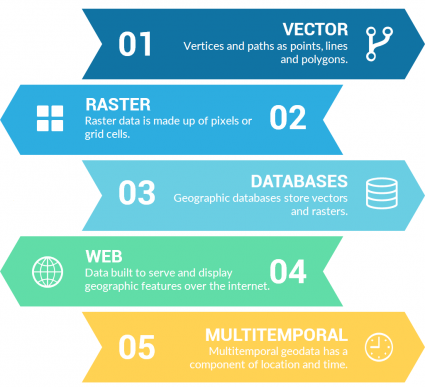
\includegraphics[width=8cm]{figures/Tugas1/1174079/vector.png}
	\centering
	\caption{Tipe data Geospasial.}
\end{figure}	

	\item Vector merupakan tipe data yang mencakup vertices dan juga path. 3 hal mendasar dari sebuat vector merupakan point, garis, dan juga polgyons. setiap point, garus dan polygon mempunyai referensi spasial seperti latitude dan longitude. Point vector berisi koordinat X dan Y, kemudian lines akan menghubungkan kedua point atau bisa juga disebut sebagai vertex, selanjutnya polgons akan menggabungkan semua vertices.
	
	\item Data Raster terbuat dari piksel dan juga cell grid. raster kebanyakan berbentuk kotak, atau bisa juga kubus. Raster akan memberikan nilai kesetiap pixes yang ada, Continuous raster mempunyai nilai yang akan selalu berubah seperti ketinggian dan temperatur. tetapi diskrit raster membuat setiap piksel menjadi class yang spesifik.
	\item Geografik Databases memiliki tujuan untuk menyimpan vector dan juga rasters. database menyimpan data geografik sebagai suatu data atau informasi yang terstruktur. Kita menggunakan database geografik karena database ini mempermudah penarikan data menjadi satu bungkusan atau package sehingga menjadi lebih mudah untuk membuat versi tersendiri ataupun hal-hal lain.
	\item Web Files seperti GeoJSON , GeoRSS dan web mapping services digunakan untuk melayani dan memperlihatkan data geografis melalui internet.
	\item Multitemporal Data menyisipkan komponen waktu ke suatu informasi geografis seperti contohnya data cuaca dan musim yang perlu di monitor temperatur dan juga informasi meteorologinya yang selalu berubah seiring dengan berjalannya waktu


	\end{enumerate}
\end{itemize}

\subsection{Link}
https://youtu.be/vzRFyiYVAUY
\subsection{Plagiarism}'\begin{figure}[H]
	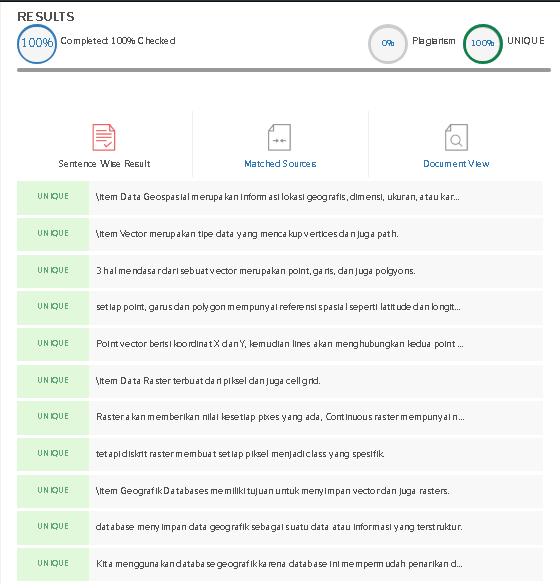
\includegraphics[width=8cm]{figures/Tugas1/1174079/plagiarisme.png}
	\centering
	\caption{Plagiarisme.}
\end{figure}	

\subsection{Cara Penggunaan}
\subsubsection{Gambar}

\hfill\break

Contoh Gambar
\begin{figure}[H]
	
\includegraphics[width=4cm]{figures/himatif.png}
	\centering
	\caption{Contoh gambar.}
\end{figure}

\subsubsection{List}
\begin{enumerate}
	\item Satu
	\item Dua
\end{enumerate}

\begin{itemize}
	\item Satu
	\item Dua
\end{itemize}


\section{Advent Nopele Olansi Damiahan Sihite (1174089)}
\subsection{Buku}
Rp.0 (Belum Lunas)
\subsection{Sejarah}
\begin{itemize}

	\item35000 tahun yang lalu, di dinding gua Lascaux, Perancis, para pemburu Cro-Magnon menggambar hewan mangsa mereka, juga garis yang dipercaya sebagai rute migrasi hewan-hewan.
	\item	Pada tahun 1700-an teknik survey modern untuk pemetaan topografis diterapkan, termasuk juga versi awal pemetaan tematis, misalnya untuk keilmuan atau data sensus.
	\item	Awal abad ke-20 memperlihatkan pengembangan “litografi foto” dimana peta dipisahkan menjadi beberapa lapisan (layer). Perkembangan perangkat keras komputer yang dipacu oleh penelitian senjata nuklir membawa aplikasi pemetaan menjadi multifungsi pada awal tahun 1960-an.
	\item	Tahun 1967 merupakan awal pengembangan SIG yang bisa diterapkan di Ottawa, Ontario oleh Departemen Energi, Pertambangan dan Sumber Daya, Digunakan untuk menyimpan, menganalisis dan mengolah data.
	\item	GIS dengan gvSIG.CGIS merupakan sistem pertama di dunia dan hasil dari perbaikan aplikasi pemetaan yang memiliki kemampuan timpang susun (overlay), penghitungan, pendijitalan/pemindaian (digitizing/scanning), mendukung sistem koordinat national yang membentang di atas benua Amerika.
	\item	CGIS bertahan sampai tahun 1970-an dan memakan waktu lama untuk penyempurnaan setelah pengembangan awal, dan tidak bisa bersaing denga aplikasi pemetaan komersil yang dikeluarkan beberapa vendor seperti Intergraph.


\end{itemize}
\subsection{Link}
http://tiny.cc/rodhez
\subsection{Plagiarism}'\begin{figure}[H]
	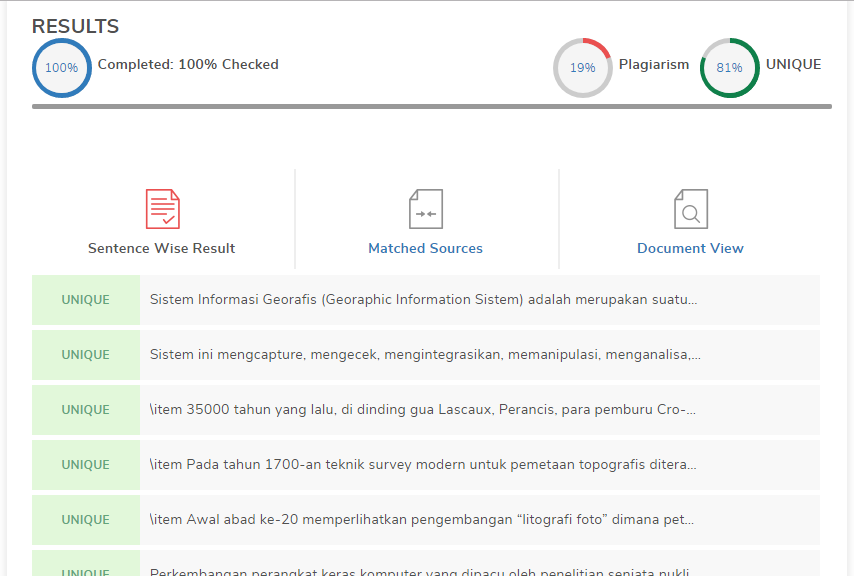
\includegraphics[width=8cm]{figures/Tugas1/1174089/plagiarisme.png}
	\centering
	\caption{Plagiarisme.}
\end{figure}	

\subsection{Cara Penggunaan}
\subsubsection{Gambar}

\hfill\break


Contoh Gambar
\begin{figure}[H]
	
\includegraphics[width=4cm]{figures/himatif.png}
	\centering
	\caption{Contoh gambar.}
\end{figure}

\subsubsection{List}
\begin{enumerate}
	\item Satu
	\item Dua
\end{enumerate}

\begin{itemize}
	\item Satu
	\item Dua
\end{itemize}


\section{Tia Nur Candida (1174086)}
\subsection{Buku}
Rp.100.000(Lunas)
\subsection{Pengertian}
	Sistem Informasi Geografis diartikan sebagai sistem untuk menyimpan, memeriksa, mengintegrasi, memanipulasi, menganalisis, dan memaparkan data yang berkaitan dengan semua ruang yang berhubungan dengan bumi. 

\subsection{Sejarah}
	Peta merupakan penggambaran sejarah secara grafis atau bentuk skala pada konsep mengenai bumi dalam hal ini peta merupakan alat untuk menyampaikan atau menginformasikan mengenai ilmu kebumian peta. Menurut Claudius ptolemy Claudius ptolomeus yang dikenal dengan nama polemik ptolemy hidup antara tahun 100 m dan 168 m beliau merupakan salah satu sarjana sains pada masanya dia tinggal dan bekerja di Alexandria di kota Mesir yang merupakan pusat intelektual dunia barat dengan perpustakaan paling luas yang pernah diciptakan ptolemy membawa semua pengetahuan dan keterampilan matematika dan astronomi dan menerapkannya pada pembuatan peta, Dia memiliki daya tarik matematikawan dengan presisi untuk menunjukkan hubungan satu tempat ke tempat lain berdasarkan perhitungan lingkaran dunia 18000 mil Ia juga mengembangkan sistem Grid latitude dan longitude yang dirancang oleh marinus of the fire sementara beberapa rincian peta Mungkin sedikit aneh dengan garis lintang yang sejajar dengan garis Khatulistiwa dengan garis bujur yang membentang ke utara selatan dengan busur Anggun sudah tidak asing lagi bagi siapa saja yang pernah memiliki Atlas ptolemy mampu membangun koordinat dan mendaftarkan lebih dari 8000 tempat dengan koordinat masing-masing 
data-data tentang pembuatan peta sempat hilang ketika perpustakaan Alexandria yang terkenal dibakar oleh orang-orang Kristen fanatik pada tahun 390 masehi sebuah contoh awal konflik antara iman dan sains tetapi satu salinan yang telah dibuat dari karya ptolemy terselamatkan dan bertahan di byzantium

\subsection{Koordinat}
	Sistem koordinat dimaksudkan untuk memberikan pengalamatan terhadap setiap lokasi di permukaan bumi dimana pengalamatan dengan sistem koordinat didasarkan pada jarak Timur Barat dan Utara Selatan suatu tempat dari suatu titik pangkal tertentu jarak diukur dalam satuan derajat sudut yang dibentuk dari titik pangkal ke posisi tersebut melalui pusat bumi sedangkan titik pangkal ditetapkan berada di perpotongan belahan utara selatan bumi atau garis Khatulistiwa dengan garis yang membelah bumi Timur Barat koordinat diambil untuk menjadi bilangan riil dalam matematika dasar tetapi memungkinkan bilangan kompleks atau elemen dari sistem yang lebih abstrak penggunaan sistem koordinat memungkinkan masalah dalam angka untuk diterjemahkan kedalam masalah-masalah tentang geometri dan juga sebaliknya.
	Garis lintang dapat disebut juga sebagai garis khatulistiwa 0 derajat atau bisa disebut juga sebagai garis tengah bumi yang membagi antara belahan bumi bagian atas dan bumi bagian bawah garis lintang digunakan sebagai penanda dalam zona iklim di dunia dari + 23 setengah derajat lintang utara sampai Min 23 setengah Lintang Selatan memiliki zona iklim tropis zona iklim tropis hanya memiliki dua musim yaitu kemarau atau panas dan penghujan saja Kemudian dari + 23 setengah derajat lintang utara sampai dengan + 66 setengah derajat Lintang Utara memiliki zona iklim subtropis Sama halnya bagian utara bagian Selatan yaitu Min 23 setengah derajat Lintang Selatan sampai 66 setengah derajat Lintang Selatan memiliki zona iklim subtropis daerah subtropis memiliki 4 musim yaitu spring Summer fall and winter. garis bujur bisa digunakan untuk menentukan waktu dan tanggal di dunia yang kita huni sekarang Jika garis lintang atau Latitude atau daerah khatulistiwa dianggap sebagai 0 derajat maka garis bujur merupakan 0 derajat yang menghubungkan Kutub Utara dengan kutub selatan yang melewati kota Greenwich di Inggris garis bujur bagian Barat kota Greenwich disebut sebagai bujur barat sedangkan garis bujur yang berada di sebelah timur kota Greenwich disebut sebagai bujur timur

\subsection{Geospasial}
	Informasi geospasial yang biasanya dikenal dengan Peta adalah informasi objek permukaan bumi yang mencakup aspek waktu dan keruangan pengertian gaya dalam geospasial berarti geosfer yang mencakup atmosfer lapisan udara yang meliputi permukaan bumi litosfer lapisan kulit bumi pedosfer tanah beserta pembentukan dan zona-zona nya sebagai bagian dari kulit bumi litosfer lapisan air yang menutupi permukaan bumi dalam berbagai bentuknya biosfer segenap unsur di permukaan bumi yang membuat kehidupan dan proses biotik berlangsung dan antroposfer manusia dengan segala aktivitas yang dilakukannya di permukaan bumi.


\subsection{Link}
https://www.youtube.com/watch?v=zrXFgPf4fLs
\subsection{Plagiarism}
\begin{figure}[H]
	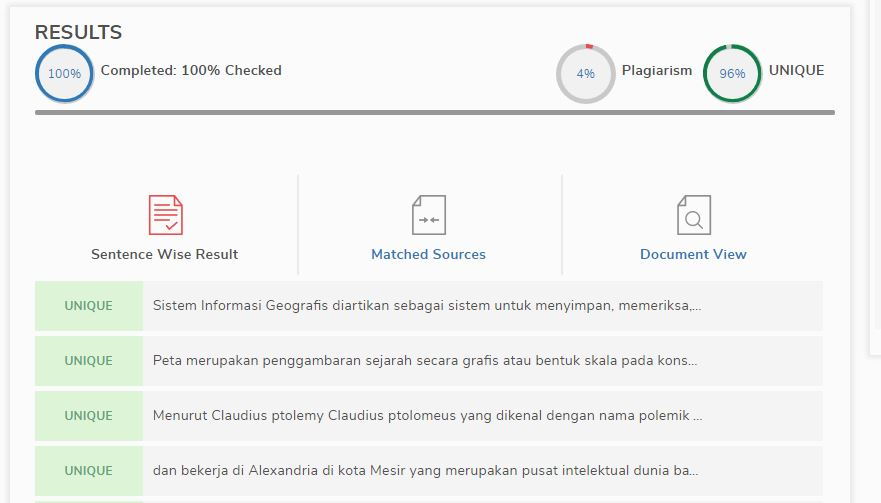
\includegraphics[width=4cm]{figures/Tugas1/1174086/plagiat.jpg}
	\centering
	\caption{Gambar Plagiat}
\end{figure}
\section{Kaka Kamaludin (1174067)}
\subsection{Buku}
belum bayar
\subsection{Data Geospasial}
Data geospasial (GD) adalah informasi yang entah bagaimana dilampirkan ke lokasi objek tertentu. Biasanya, informasi ini disimpan dalam bentuk koordinat geografis dan topologi. Jumlah data tersebut tumbuh pada tingkat yang mengejutkan, karena sebagian besar dibuat bukan oleh orang-orang, tetapi oleh berbagai perangkat.
Data geografis berisi empat komponen terintegrasi:
\begin{itemize}
	\item lokasi
	\item properti dan karakteristik
	\item hubungan sosial
	\item waktu
\end{itemize}
Dengan demikian, dalam GIS, data geospasial direpresentasikan dalam dua kategori yaitu spasial(lokasi) dan non-spasial(atribut). Data spasial dapat mencakup fitur geografis yang diwakili oleh:
\begin{itemize}
 	\item titik, mewakili pohon, tiang lampu, atau beberapa objek yang lokasinya dijelaskan oleh satu titik.
 	\item garis,  adalah objek nyata yang dapat dianggap sebagai garis. Busur terdiri dari segmen garis dan busur lingkaran. Di dunia nyata, busur dapat berupa jalan, sungai, saluran transmisi listrik atau utilitas bawah tanah, misalnya, sistem saluran air dan saluran pembuangan.
 	\item Poligon adalah area tertutup yang mewakili area yang homogen dengan beberapa kriteria. Poligon menunjukkan jenis tanah, konstituensi, plot tanah atau kontur bangunan.
\end{itemize}
Data atribut dapat mencakup pengidentifikasi objek, informasi deskriptif apa pun dari basis data, gambar, dan banyak lagi.
\subsection{Link}
https://cutt.ly/kepEJNS
\subsection{Plagiarism}
\begin{figure}[H]
	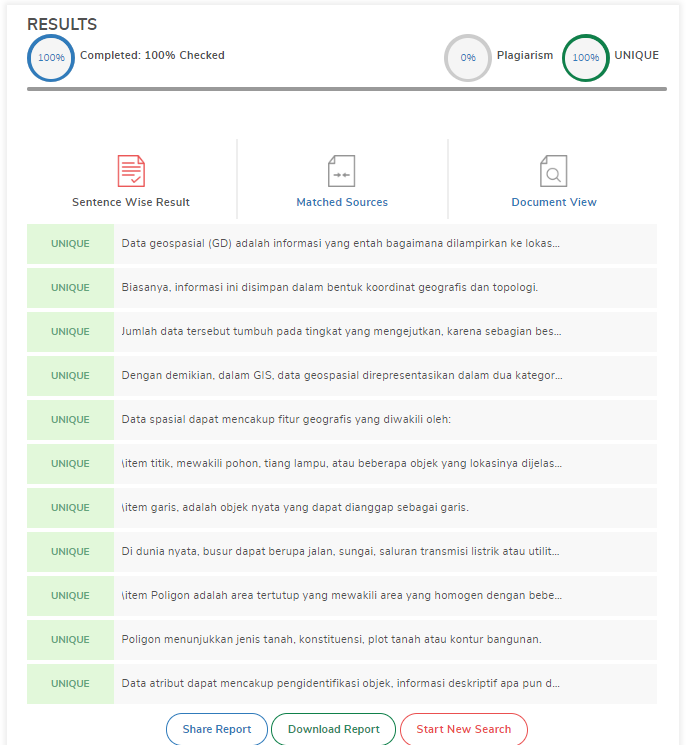
\includegraphics[width=4cm]{figures/Tugas1/1174067/plagiat.png}
	\centering
	\caption{Gambar Plagiat}
\end{figure}
\section{Fanny Shafira Damayanti (1174069)}
\subsection{Buku}
Belum Lunas
\subsection{Pengertian Sistem Informasi Geografis}
Sistem Informasi Geografis merupakan system yang memiliki kemampuan untuk menyimpan, membangun, mengelola semua informasi yang bereferensi geografis.
\subsection{Sejarah}
Awal dikenalnya SIG tidak lepas dari adanya kemajuan dalam bidang teknologi terutama komputer. Selama perang dunia kedua pemrosesan data mengalami kemajuan yang pesat terutama untuk memenuhi kebutuhan militer dalam memprediksi trayektori balistik. Pada awal tahun 1960-an perkembangan dalam ilmu komputer semakin pesat dan siap digunakan untuk bidang lain di luar militer. Para ahli meteorologi, geologi, dan geofisika mulai menggunakan komputer dalam pembuatan peta.
Tahun 1963 di Kanada muncul CGIS (Canadian Geographic Information System), dan selanjutnya menjadi SIG pertama di dunia. Dua tahun kemudian di Amerika Serikat beroperasi sistem serupa bernama MIDAS yang digunakan untuk memproses data-data sumber daya alam.
Seiring dengan berkembangnya teknologi, GIS juga mengalami perubahan ke arah yang lebih baik. Berikut adalah sejarah perkembangan GIS dari masa ke masa :
\begin{itemize}
\item 35000 tahun yang lalu, di dinding gua Lascaux, Perancis, para pemburu Cro-Magnon menggambar hewan mangsa mereka, juga garis yang dipercaya sebagai rute migrasi hewan-hewan tersebut. Catatan awal ini sejalan dengan dua elemen struktur pada sistem informasi gegrafis modern sekarang ini, arsip grafis yang terhubung ke database atribut.

\item Pada tahun 1700-an teknik survey modern untuk pemetaan topografis diterapkan, termasuk juga versi awal pemetaan tematis, misalnya untuk keilmuan atau data sensus.

\item Awal abad ke-20 memperlihatkan pengembangan “litografi foto” dimana peta dipisahkan menjadi beberapa lapisan (layer). Perkembangan perangkat keras komputer yang dipacu oleh penelitian senjata nuklir membawa aplikasi pemetaan menjadi multifungsi pada awal tahun 1960-an.

\item Tahun 1967 merupakan awal pengembangan SIG yang bisa diterapkan di Ottawa, Ontario oleh Departemen Energi, Pertambangan dan Sumber Daya. Dikembangkan oleh Roger Tomlinson, yang kemudian disebut CGIS (Canadian GIS – SIG Kanada), digunakan untuk menyimpan, menganalisis dan mengolah data yang dikumpulkan untuk Inventarisasi Tanah Kanada (CLI – Canadian land Inventory) – sebuah inisiatif untuk mengetahui kemampuan lahan di wilayah pedesaan Kanada dengan memetakaan berbagai informasi pada tanah, pertanian, pariwisata, alam bebas, unggas dan penggunaan tanah pada skala 1:250000. Faktor pemeringkatan klasifikasi juga diterapkan untuk keperluan analisis.

\item GIS dengan gvSIG.CGIS merupakan sistem pertama di dunia dan hasil dari perbaikan aplikasi pemetaan yang memiliki kemampuan timpang susun (overlay), penghitungan, pendijitalan/pemindaian (digitizing/scanning), mendukung sistem koordinat national yang membentang di atas benua Amerika , memasukkan garis sebagai arc yang memiliki topologi dan menyimpan atribut dan informasi lokasional pada berkas terpisah. Pengembangya, seorang geografer bernama Roger Tomlinson kemudian disebut “Bapak SIG”.

\item CGIS bertahan sampai tahun 1970-an dan memakan waktu lama untuk penyempurnaan setelah pengembangan awal, dan tidak bisa bersaing denga aplikasi pemetaan komersil yang dikeluarkan beberapa vendor seperti Intergraph. Perkembangan perangkat keras mikro komputer memacu vendor lain seperti ESRI dan CARIS berhasil membuat banyak fitur SIG, menggabung pendekatan generasi pertama pada pemisahan informasi spasial dan atributnya, dengan pendekatan generasi kedua pada organisasi data atribut menjadi struktur database. Perkembangan industri pada tahun 1980-an dan 1990-an memacu lagi pertumbuhan SIG pada workstation UNIX dan komputer pribadi. Pada akhir abad ke-20, pertumbuhan yang cepat di berbagai sistem dikonsolidasikan dan distandarisasikan menjadi platform lebih sedikit, dan para pengguna mulai mengekspor menampilkan data SIG lewat internet, yang membutuhkan standar pada format data dan transfer. 

\end{itemize}

\subsection{Koordinat}
\begin{itemize}
\item Garis Lintang (Latitude)
\item Garis Lintang (Latitude)
\begin{figure}[H]
	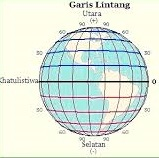
\includegraphics[width=4cm]{figures/Tugas1/1174069/lintang.jpg}
	\centering
	\caption{Gambar Garis Lintang}
\end{figure}
Garis lintang merupakan garis yang menentukan lokasi bumi terhadap garis khatulistiwa (utara atau selatan). 

\item Garis Bujur (Longtitude)
\begin{figure}[H]
	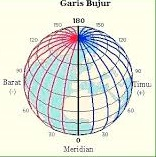
\includegraphics[width=4cm]{figures/Tugas1/1174069/bujur.jpg}
	\centering
	\caption{Gambar Garis Bujur}
\end{figure}
Garis Bujur, menggambarkan lokasi sebuah tempat di timur atau barat Bumi dari sebuah garis utara-selatan yang disebut Meridian Utama. 
\end{itemize}

\subsection{Data Geospasial}
UU No. 4 Tahun 2011 Tentang Informasi Geospasial pasal 1-4 menerangkan, spasial adalah aspek keruangan suatu objek atau  kejadian yang mencakup lokasi, letak, dan posisinya. Geospasial atau ruang kebumian adalah aspek keruangan yang menunjukkan lokasi, letak, dan posisi suatu objek atau kejadian yang berada di bawah, pada, atau di atas permukaan bumi yang dinyatakan dalam sistem koordinat tertentu. Data Geospasial yang selanjutnya disingkat “DG”, adalah data tentang lokasi geografis, dimensi atau ukuran, dan/atau karakteristik objek alam dan/atau buatan manusia yang berada di bawah, pada, atau di atas permukaan bumi. Informasi Geospasial yang selanjutnya disingkat IG adalah DG yang sudah diolah sehingga dapat digunakan sebagai alat bantu dalam perumusan kebijakan, pengambilan keputusan, dan/atau pelaksanaan kegiatan yang berhubungan dengan ruang kebumian.

Contoh data spasial antara lain letak suatu wilayah, posisi sumber minyak bumi,dsb. Bentuk-bentuk data spasial : titik (dot), contoh: posisi terminal; garis (poly line), contoh: jaringan jalan raya; dan area (polygon), contoh: wilayah kecamatan. Contoh data atribut misalnya kepadatan penduduk, jenis tanah, dsb. Bentuk-bentuk data atribut adalahdata kuantitatif (angka-angka/statistik), contoh: jumlah penduduk dan data kualitatif (kualitas/mutu), contoh: tingkat kesuburan tanah.

Jenis-Jenis Data Geospasial
\begin{itemize}
\item Data Vektor
Data vektor adalah data yang direpresentasikan sebagai suatu mosaik berupa garis (arc/line), polygon (daerah yang dibatasi oleh garis yang berawal dan berakhir pada titik yang sama), titik/point (node yang mempunyai label), dan nodes (merupakan titik perpotongan antara dua buah garis). Keuntungan utama dari format data vektor adalah ketepatan dalam merepresentasikan fitur titik, batasan dan garis lurus.

Kegunaan Data Vektor untuk analisa yang membutuhkan ketepatan posisi, misalnya pada basis data batas-batas kadaster. Contoh penggunaan lainnya adalah untuk mendefinisikan hubungan spasial dari beberapa fitur. Kelemahan data vektor yang utama adalah ketidakmampuannya dalam mengakomodasi perubahan gradual.

\item Data Raster
Data raster adalah data yang dihasilkan dari penginderaan jauh. Data Raster sering disebut juga dengan sel grid. Pada data raster, obyek geografis direpresentasikan sebagai struktur sel grid yang disebut dengan pixel (picture element). Pada data raster, resolusi (definisi visual) tergantung pada ukuran pixel-nya. Dengan kata lain, resolusi pixel menggambarkan ukuran sebenarnya di permukaan bumi yang diwakili oleh setiap pixel pada citra.

Semakin kecil ukuran permukaan bumi yang direpresentasikan oleh satu sel, semakin tinggi resolusinya. Data raster sangat baik untuk merepresentasikan batas-batas yang berubah secara gradual, seperti jenis tanah, kelembaban tanah, vegetasi, suhu tanah, dan sebagainya. Kelemahan utama dari data raster adalah besarnya ukuran file; semakin tinggi resolusi grid-nya semakin besar pula ukuran filenya.

Masing-masing format data mempunyai kelebihan dan kekurangan. Pemilihan format data yang digunakan sangat tergantung pada tujuan penggunaan, data yang tersedia, volume data yang dihasilkan, ketelitian yang diinginkan, serta kemudahan dalam analisa. Data vektor relatif lebih ekonomis dalam hal ukuran file dan presisi dalam lokasi, tetapi sangat sulit untuk digunakan dalam komputasi matematik. Sebaliknya, data raster biasanya membutuhkan ruang penyimpanan file yang lebih besar dan presisi lokasinya lebih rendah, tetapi lebih mudah digunakan secara matematis.

\item Titik (dimensi nol - point)
Titik adalah representasi grafis atau geometri yang paling sederhana bagi objek spasial. Representasi ini tidak memiliki dimensi, tetapi dapat diidentifikasikan di atas peta dan dapat ditampilkan pada layar monitor dengan menggunakan simbol-simbol tertentu. Perlu dipahami juga bahwa skala peta akan menentukan apakah suatu objek akan ditampilkan sebagai titik atau polygon. Pada peta skala besar, unsur-unsur bangunan akan ditampilkan sebagai polygon, sedangkan pada skala kecil akan ditampilkan sebagai unsur-unsur titik.
Format titik : koordinat tunggal, tanpa panjang, tanpa luasan.
Contoh : lokasi kecelakaan, letak pohon

\item Garis (satu dimensi – line atau polyline)
Garis adalah bentuk geometri linier yang akan menghubungkan paling sedikit dua titik dan digunakan untuk merepresentasikan objek-objek yang berdimensi satu. Batas-batas objek geometri polygon juga merupakan garis-garis, demikian pula dengan jaringan listrik, jaringan komunikasi, pipa air minum, saluran buangan, dan utility lainnya dapat direpresentasikan sebagai objek dengan bentuk geometri garis. Hal ini akan bergantung pada skala peta yang menjadi sumbernya atau skala representasi akhirnya.

Format : Koordinat titik awal dan akhir, mempunyai panjang tanpa luasan.
Contoh : jalan, sungai, utility

\item Polygon (dua dimensi – area)
Geometri polygon digunakan untuk merepresentasikan objek-objek dua dimensi. Unsurunsur spasial seperti danau, batas propinsi, batas kota, batas persil tanah milik adalah beberapa contoh tipe entitas dunia nyata yang pada umumnya direpresentasikan sebagai objek-objek dengan geometri polygon. Meskipun demikian, representasi ini masih akan bergantung pada skala petanya atau sajian akhirnya.

Format : Koordinat dengan titik awal dan akhir sama, mempunyai panjang dan luasan.
Contoh : Tanah persil, bangunan

\end{itemize}
\subsection{Link}
https://youtu.be/m0sEiWnj3Aw

\subsection{Plagiarism}
\subsection{Plagiarism}
\begin{figure}[H]
	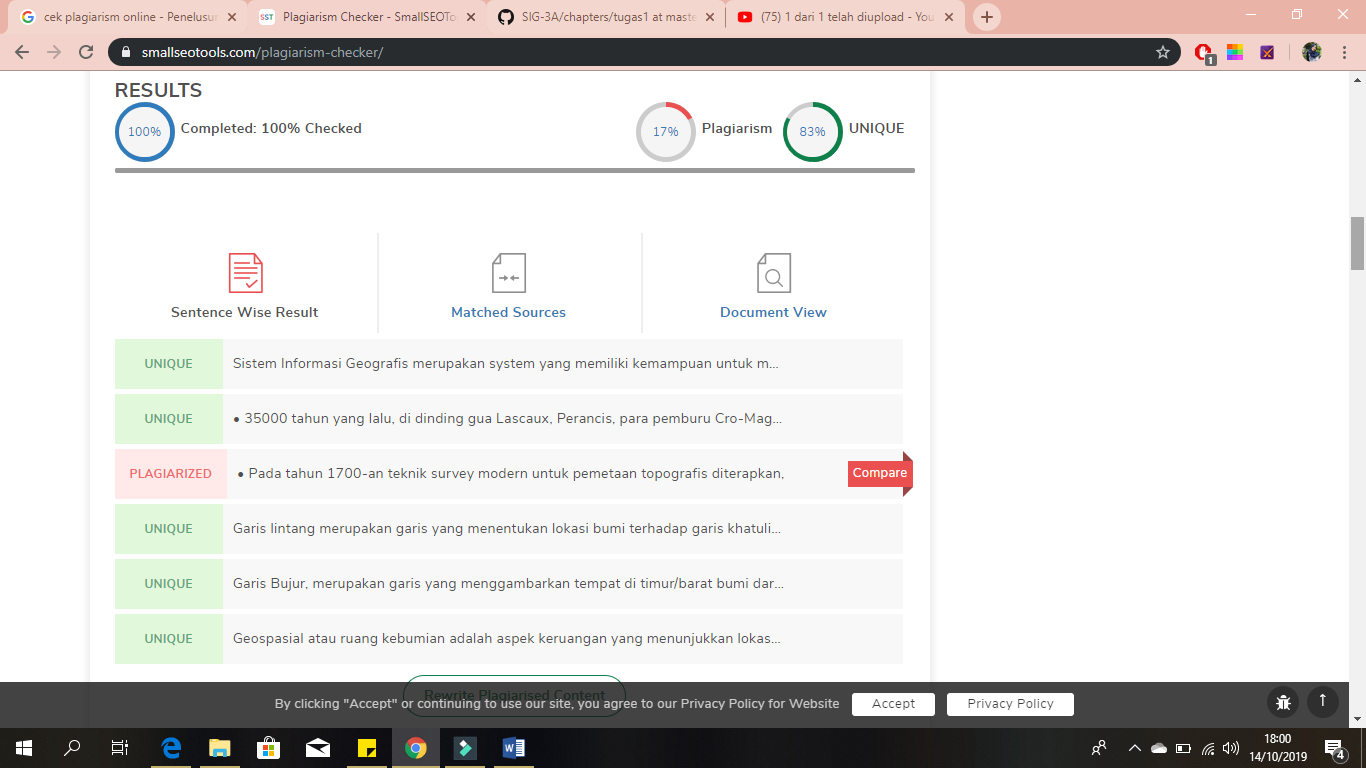
\includegraphics[width=4cm]{figures/Tugas1/1174069/plagiarism.png}
	\centering
	\caption{Gambar Plagiat}
\end{figure}


\section{Ilham Muhammad Ariq (1174087)}
\subsection{Buku}
Rp.0 (Belum Lunas)
\subsection{Data Geospasial}
\begin{itemize}
	\item Pengertian Data Geospasial
	\par Geospasial terdiri dari dua kata, yaitu geo dan spasial, Geo berarti bumi sedangkan Spasial berarti ruang. UU No 4 tahun 2011 tentang geospasial menyebutkan, spasial adalah aspek keruangan dari suatu objek, atau yang mencakup lokasi,letak, dan posisinya. Data Geospasial dipecah menjadi dua, yaitu yang pertama;Data grafis atau geometri.Data ini terdiri dari tiga elemen: titik, garis, dan luasan. Data ini berbentuk vektor maupun raster. Kedua data tersebut adalah data atribut atau data tematik. Berikut penjelasan kedua data tersebut.
	
	\begin{enumerate}
	\item Data Vector
	\par Dalam bentuk data vector bagian objek dibumi ditampilkan sebagai kumpulan titik , garis dan polygon dimana sekumpulan tiitik yang saling terhubung akan membentuk garis dan garis yang saling terhubung antara titik awal dan titik akhir dengan nilai koordinat ynag sama akan membentuk polygon

	\begin{figure}[H]
	
\includegraphics[width=4cm]{figures/Tugas1/1174087/vektor.png}
	\centering
	\caption{Data Vektor}
	\end{figure}
	
Data Vektor dibagi menjadi 2 yaitu :
	\begin{enumerate}
	\item Culture
	\par Culture memaparkan atau menampilkan data geospasial yang disertai dengan nama atribut atau memberikan 	keterangan atas nama dari objek di bumi. Contohnya nama dari suatu Negara, indicator batas air(keterangan kedalaman air laut), nama provinsi, daerah, wilayah dsb.
	
	\begin{figure}[H]
	
\includegraphics[width=4cm]{figures/Tugas1/1174087/lp.jpg}
	\centering
	\caption{Culture}
	\end{figure}
	
	\item Physical
	\par Physical memaparkan atau menampilkan data geospasial mengenai bentuk fisiknya atau gambaran tentang objek-objek alam yang ada dibumi. Contohnya gambaran laut, garis pantai, terumbu karang, danau dsb.
	
	\begin{figure}[H]
	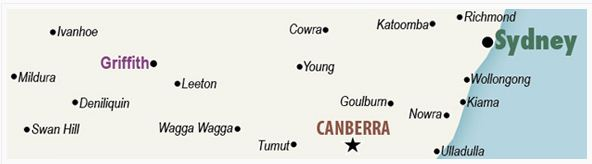
\includegraphics[width=4cm]{figures/Tugas1/1174087/pc.jpg}
	\centering
	\caption{Physycal}
	\end{figure}
	\end{enumerate}
	
	\item Data Raster
	\par Data raster menampilkan permukaan bumi seperti bentuk aslinya atau seperti dalam peta asli yang terlihat jelas dari setiap objek dengan keadaan alamnya. Data raster dibentuk atau menampilkan objek berupa elemen matriks atau grid , data raster digunakan untuk merepresentasikan objek dari data geospasial mengenai batas-batas yang berubah, ketinggian tanah dsb.

	\begin{figure}[H]
	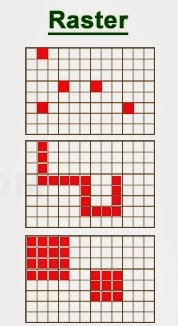
\includegraphics[width=4cm]{figures/Tugas1/1174087/raster.png}
	\centering
	\caption{Data Raster}
	\end{figure}
	\end{enumerate}
	
Dan adapaun software yang digunakan untuk mengolah data spasial atau membuat map kustom contohnya dapat menggunakan software QGIS dimana data yang akan diolah bisa didapatkan di web Natural Earth , ada data spasial berupa vector yang dibuat oleh ESRI (Environmental System Research Institute, Inc) dengan format data shapefile dan untuk data raster ada dengan format TIFF dengan TFW world file.
	
\end{itemize}

\subsection{Link}
\verb|https://youtu.be/iC4c71hMc_k|

\subsection{Plagiarism}
\begin{figure}[H]
	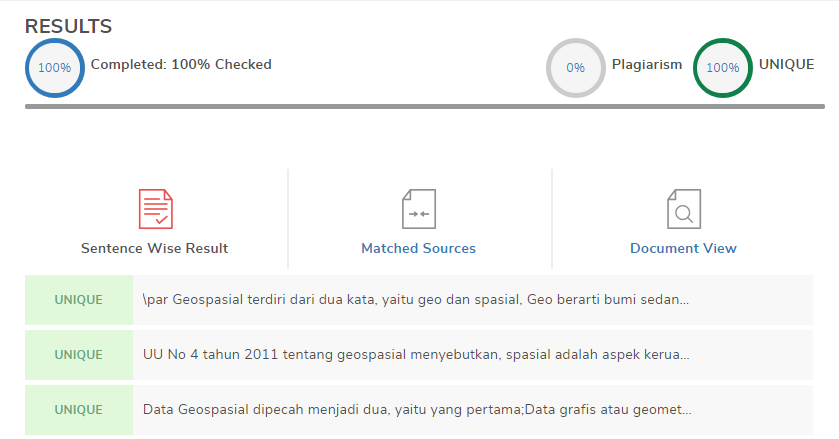
\includegraphics[width=4cm]{figures/Tugas1/1174087/plagiarism.png}
	\centering
	\caption{Plagiarism}
	\end{figure}
\section{Alvan Alvanzah/1174077}
\subsection{BUKU}
Rp. 0 (Belum Lunas)

\subsection{SEJARAH PTOLEMY}
\begin{itemize}
    \item Peta
    
Peta merupakan penggambaran secara grafis atau bentuk skala (perbandingan) pada konsep mengenai bumi dalam hal ini peta merupakan alat untuk menyampaikan atau menginformasikan mengenai ilmu kebumian.
    \item Peta Menurut Claudius Ptolemaeus Ptolemy
    
Cladius Ptolemaeus yang dikenal dengan nama Ptolemy, hidup antara tahun 100 masehi dan 168 masehi, beliau merupakan salah satu sarjana sains pada masanya. Ptolemy membawa semua pengetahuan dan keterampilan matematika dan astronomi dan menerapkanya pada pembuatan peta. Data-data tentang pembuatan peta sempat hilang ketika perpustakaan Alexandria yang terkenal dibakar oleh orang-orang Kristen fanatik pada tahun 390 masehi-sebuah contoh awal konflik antara iman dan sains.
    \item Peta Dunia Ptolemy
    
Peta dunia Ptolemy adalah peta dunia yang diketahui masyarakat barat pada waktu kurun kedua masehi. Peta tersebut berdasarkan penerangan yang terkandung di dalam buku geographia, ditulis kira-kira pada 150 masehi walaupun peta autentik tidak dijumpai, buku geographia yang berisi beribu-ribu rujukan dari berbagai tempat di dunia, beserta koordinat, yang membolehkan para pelukis peta menyusun semula peta dunia Ptolemy apabila manuskripnya telah ditemui sekitar 1300 masehi.
    \item Sejarah Ptolemy

Clauduis Ptolemy adalah seorang ahli geografi, astronom, dan astrolog yang hidup pada zaman Helenistik di provinsi Romawi, Aegyptus. Claudius merupakan nomen atau nama keluarga seorang Roma, Ptolemaeus menyandang nama itu, sehingga menjadi bukti bahwa dia adalah seorang warga negara roma. Ptolemaeus (Ptolemy) adalah sebuah nama Yunani. Muncul satu kali di mitologi Yunani, dalam bentuk Homeric. Selain itu dianggap juga sebagai seorang anggota masyarakat Yunani alexandria, dan hanya sedikit yang mengetahui rincian hidup Ptolemaeus. Karya utama Ptolemy lainnya adalah Geografinya (juga disebut Geographia), kompilasi koordinat geografis dari bagian dunia yang dikenal oleh kekaisaran Romawi pada masanya.
    \item The Geography
    
Bagian pertama dari Geografi adalah diskusi tentang data dan metode yang digunakan. Seperti  model tata surya di Almagest, Ptolemy memasukkan semua informasi ini ke dalam skema besar. Ptolemaeus juga merancang dan memberikan petunjuk bagaimana membuat peta di seluruh dunia yang berpenghuni dan berprovinsi Romawi. Peta di manuskrip yang masih ada di Ptolemy’s Geography, bagaimanapun, hanya bersal dari sekitar tahun 1300, setelah teks tersebut ditemukan kembali oleh Maximus Planudes. Peta berdasarkan prinsip ilmiah telah dibuat sejak zaman Eratosthenes, pada abad ke-3 sebelum masehi, namun Ptolemy memperbaiki proyeksi peta. Karena Ptolemy berasal dari garis lintang utamanya dari nilai terpanjang minyak mentah, garis lintangnya rata-rata keliru kira-kira satu derajat, meskipun para astronom kuno mampu mengetahui garis lintang mereka lebih lama.
\end{itemize}

\subsection{Link Video}
Link Video : \texttt{https://youtu.be/TBVqN9eWO8g}

\subsection{Plagiarisme}
\begin{figure}[!htbp]
\centering
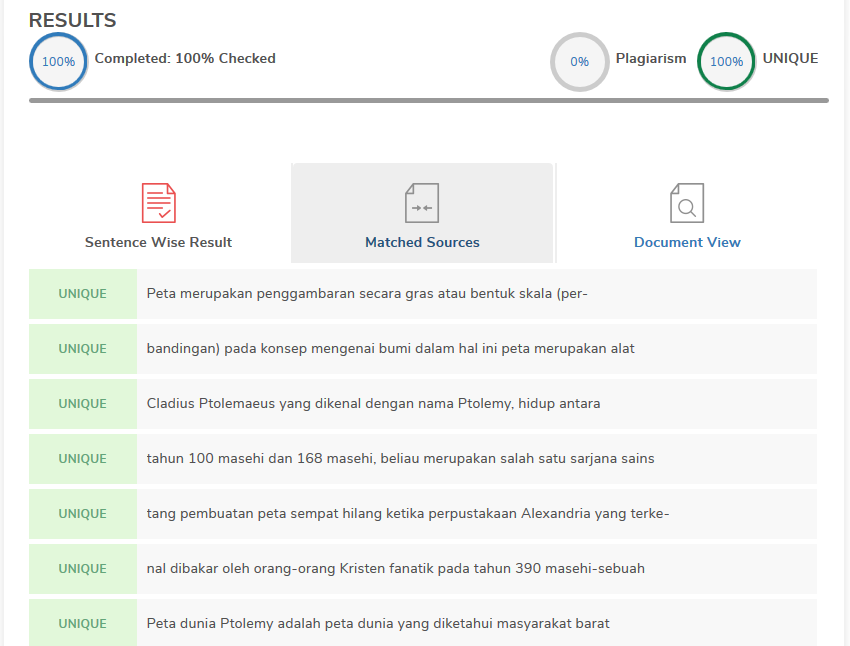
\includegraphics[width=12cm,height=8cm]{figures/tugas1/1174077/plagarisme.PNG}
\caption{Hasil Plagiarisme}
\label{penanda}
\end{figure}

\section{Muhammad Reza Syachrani (1174084)}
\subsection{Buku}
Rp.100.000(Lunas)
\subsection{Pengertian}
    \hspace{1cm} Sistem Informasi Geografis (SIG) atau Geographic Information System (GIS) adalah sebuah computer yang berbasis system informasi digunakan untuk memberikan informasi bentuk digital dan analisis terhadap permukaan geografis bumi, SIG diartikan sebagai system untuk menyimpan, memeriksa, mengintegrasi, mamanipulasi, menganalisis, dan memaparkan data yang semua berkaitan atau berhubungan dengan keadaan bumi.\\
    Definisi dari Sistem Informasi Geografis (SIG) lainnya, yaitu :
    \begin{itemize}
        \item Menurut (Rhind, 1998), GIS is a computer system for collecting, checking, integrating and analysing information related to the surface of the earth.
        \item Menurut (Marble and Peuquet, 1983) dan (Parker, 1988; Ozemoy et al., 1981; Burrough, 1986), GIS deals with space-time data and often but not necessarily, employs computer hardware and software.
    \end{itemize}
    \par Sistem Informasi Geografis merupakan pemahaman dari 3 rangkaian kata, sebagai berikut :
    \begin{enumerate}
        \item Geografi\\
        SIG dibangun berdasarkan pada istilah ‘geografi’ dan ‘spesial’. Objek mengacu pada spesifikasi lokasi dalam suatu tempat/ruang. Penampakan yang seperti ditampilkan pada suatu peta yang digunakan untuk memberi gambaran yang lebih representasi dari suatu objek yang sesuai dengan kenyatan di bumi.
        \item Informasi\\
        Informasi merupakan kata yang berasal dari kata pengolahan sejumlah data. Di dalam Sistem Informasi Geografis informasi memiliki volume yang besar karna setiap objek geografis memiliki setting datanya tersendiri. Maka, semua data harus dialokasikan pada objek special yang mampu membuat peta menjadi intelligent.
        \item Sistem
        Sistem merupakan kumpulan elemen-elemen yang berintegrasi dan berinterdependensi dalam sebuah lingkungan yang dinamis untuk mencapai tujuan tertentu.
    \end{enumerate}
    \par Sistem Informasi Geografis juga terdiri dari 5 komponen, yaitu :
    \begin{enumerate}
        \item Sistem Komputer (Perkakas dan System operasi)
        \item Software GIS (ArcGIS)
        \item Database GIS
        \item Methods GIS (Prosedur analisis)
        \item People (Orang-orang yang menggunakan GIS/User)
    \end{enumerate}
    \par Dalam Sistem Informasi Geografis terdapat data special yang terbagi menjadi 2 model data yang digunakan untuk mempresentasikan real word, yaitu:
    \begin{enumerate}
        \item Vektor\\
        Model data vector merupakan model data yang banyak digunakan, model ini berbasiskan pada titik dengan koordinat (x,y) untuk membangun sebuah objek special. Sebagai contoh bumi dalam data vector dipresentasikan sebagai mozaik yang terdiri dari garis, polygon, titik dan noders. Keuntung dari menggunakan model data vector yaitu ketepatan dalam merepresentasikan fitur titik, batasan dan garis  lurus.
        \item Raster\\
        Model data raster adalah data yang dihasilkan dari system pengindraan jauh. Pada data raster, struktur sel grid yang disebut pixel  merupaka representasi objek geografis. Data raster cocok untuk mempresentasikan batas-batas yang berubah secara gradual, seperti jenis tanah, vegetasi, suhu tanah, dan kelembapan tanah.
    \end{enumerate}
    \subsection{Link}
    LINK VIDEO :  \texttt{https://youtu.be/23n\_Ik\_Nbf0}
    \subsection{Plagiarism}
    \begin{figure}[H]
	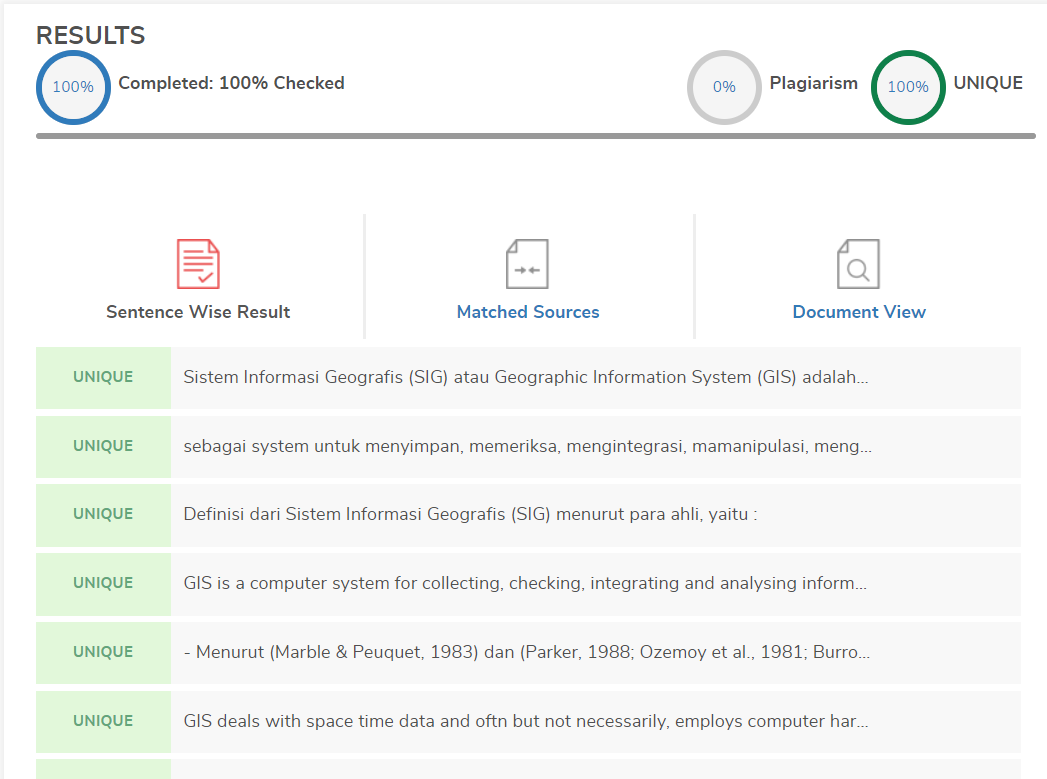
\includegraphics[width=4cm]{figures/Tugas1/1174084/plagiarism.png}
	\centering
	\caption{Plagiarism}
    \end{figure}
 
\section{Arrizal Furqona Gifary (1174070)}
\subsection{Koordinat}
\begin{itemize}
	\item Sejarah Koordinat
Koordinat adalah suatu titik yang didapatkan dari hasil perpotongan dari garis latitude (lintang) dengan garis bujur (longitude) sehingga akan menunjukan lokasi pada suatu daerah. Umumnya koordinat dibedakan menjadi koordinat Geographic dan Universal Transver Mercator (UTM). 	
Menurut Heroditus (450-M) yaitu seorang ahli sejarah mengatakan bahwa geometri itu berasal dari Mesir. Rane Discartes (Matematikawan) adalah sesesorang yang memiliki ketertarikan di bidang geometri. Rane menemukan metode untuk menyajikan sebuah titik sebagai sebuah bilangan berpasangan dalam sebuah bidang datar. Bilangan-bilangan itu terletak pada dua garis yang saling tegak lurus antara satu dengan lainnya dan berpotongan di sebuah titik yaitu (0,0) yang dinamakan Origin, dan biasanya ditandai atau disimbold engan O (0,0). Bidang tersebut dinamakan bidang "Koordinat" atau yang biasa kita tau sebagai bidang kartesius.
	\item Sistem Koordinat Dua Dimensi
	\begin{enumerate}
	\item Sistem Koordinat Kartesius
	
Sistem koordinat ini digunakan untuk mendefinisikan jarak dari titik awal (0,0) kepada titik x yang disebut koordinat x (absis) dan titik y yang disebut koordinat y (ordinat) dari titik awal kita.
Untuk menggambarkan titik x dan y bisa dilihat pada(Gambar 1).
	\begin{figure}[H]
	\includegraphics[width=4cm]{figures/Tugas1/1174070/kartesius.png}
	\centering
	\caption{Gambar 1}
\end{figure}
	
	\item Sistem Koordinat Polar

Sistem Koordinat Polar adalah sistem koordinat 2D yang titik bidangnya itu ditentukan dari jarak titik yang telah ditentukan dan suatu sudut dari arah yang sebelumnya telah ditentukan.

Titik yang sudah ditentukan disebut pole atau kutub, dan ray atau sinar dari kutub pada arah yang sudah ditentukan disebut dengan polar axis atau aksis polar. Jarak dari sebuah kutub disebut dengan radial coordinate atau radius dan sudutnya disebut dengan angular coordinate atau polar angle atau azimuth.

Contoh untuk Koordinat polar (Gambar 2).
	\begin{figure}[H]
	\includegraphics[width=4cm]{figures/Tugas1/1174070/polar.png}
	\centering
	\caption{Gambar 1}
\end{figure}
	\end{enumerate}
\end{itemize}
\subsection{Link}
https://youtu.be/pf1TGbKMJpU
\subsection{Plagiarism}
\begin{figure}[H]
	\includegraphics[width=4cm]{figures/Tugas1/1174070/plagiat.jpg}
	\centering
	\caption{Gambar Plagiat}
\end{figure}

\section{Bakti QIlan Mufid (1174083)}
\subsection{Buku}
Rp.100.000(Lunas)
\subsection{Data Geospasial}
\begin{itemize}
\item Geospasial data atau juga bisa disebut dengan Spatial Data atau GIS (Geospatial Information System data) adalah tentan g aspek fisik dan adminsitratif dari sebuah objek geografis. Aspek fisik ini mencakup pula bentuk anthropogenic dan bentuk alam baik yang terdiri dari permukaan maupun dibawah permukaan bumi. Bentuk anthropogenic mengandung didalamnya fenomena budaya seperti jalan, rel kereta api, bangunan, jembatan, dan sebagainya. Bentuk alam tentusaja seperti sungai, danau, pantai, dataran tinggi, dan sebagainya. Sedangkan aspek administratif adalah pembagian atau pembatasan sosio-kultular yang dibuat oleh suatu organisasi atau badan untuk keperluan pengaturan dan pemakaian sumberdaya alam. Termasuk dalam aspek administratif ini adalah batas negara, pembagian wilayah administrasi, zona, kode pos, batas kepemilikan tanah, dan sebagainya.

\item SIG mulai dikenal pada awal 1980-an. Sejalan dengan berkembangnya perangkat komputer, baik perangkat lunak maupun perangkat keras, SIG berkembang sangat pesat pada era 1990-an.

\item Secara harafiah, SIG dapat diartikan sebagai : \textit{”suatu komponen yang terdiri dari perangkat keras, perangkat lunak, data geografis dan sumberdaya manusia yang bekerja bersama secara efektif untuk menangkap, menyimpan, memperbaiki, memperbaharui, mengelola, memanipulasi, mengintegrasikan, menganalisa, dan menampilkan data dalam suatu informasi berbasis geografis”} 

\item Secara umum terdapat dua metode untuk menampilkan fitur geografis ke dalam GIS atau Sistem Informasi Geospasial:
	\begin{enumerate}
	\item Data Raster  (raster data structure)Terdiri dari serangkaian sel atau pixels yang biasa dipakai untuk menggambarkan data gambar sebagai data yang berkesinambungan. Dalam struktur data yang demikian, ada unsur resolusi sebagai ukuran dari dimensi fitur geografis yang terwakili dalam bentuk pixel. Biasanya data raster ini dipakai untuk citra satelit, ortografi digital, model elevasi digital (digital elevation models, DEM), peta digital, dan sebagainya.
	\begin{figure}[H]
	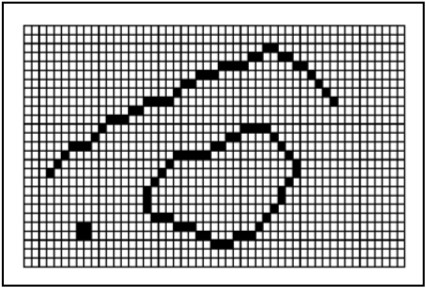
\includegraphics[width=4cm]{figures/Tugas1/1174083/Raster.jpg}
	\centering
	\caption{Data Raster}
	\end{figure}
	\item Data Vektor (vector data structure)Terdiri dari sebuah gambaran titik geografis, baik yang berupa tanda titik, garis, maupun poligon. Model grafik vektor ini menampilkan secara terpisah fitur geografis seperti batas administratif, jalan, bangunan, dan sungai. Sebuah objek grafis biasanya dikaitkan dengan informasi yang mengandung penjelasan tentang atribut objek itu, dan informasi ini bisa saja disimpan di dalam berkas spreadsheets atau pangkalan data terpisah.
	\begin{figure}[H]
	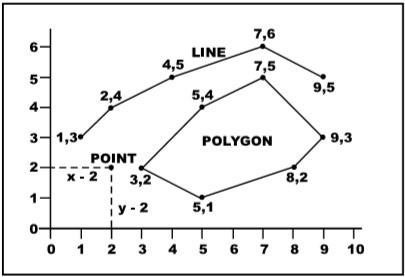
\includegraphics[width=4cm]{figures/Tugas1/1174083/vektor.jpg}
	\centering
	\caption{Data Vektor}
	\end{figure}
	\end{enumerate}
\end{itemize}

\subsection{Link}
http://bit.ly/baktiGEO
\subsection{Plagiarism}
	\begin{figure}[H]
	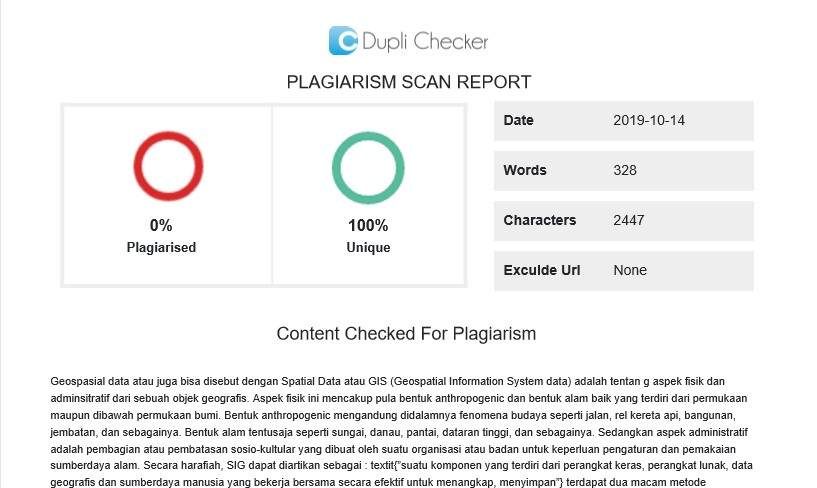
\includegraphics[width=4cm]{figures/Tugas1/1174083/plagiarsm.jpg}
	\centering
	\caption{check plagiarsm}
	\end{figure}

\subsection{Cara Penggunaan}
\subsubsection{Gambar}

\hfill\break

Contoh Gambar
\begin{figure}[H]
	
\includegraphics[width=4cm]{figures/himatif.png}
	\centering
	\caption{Contoh gambar.}
\end{figure}

\subsubsection{List}
\begin{enumerate}
	\item Satu
	\item Dua
\end{enumerate}

\begin{itemize}
	\item Satu
	\item Dua
\end{itemize}


\section{Alfadian Owen (1174091)}
\subsection{Buku}
Rp.100.000(Lunas)
\subsection{Data Geospasial}
\begin{itemize}
	\item Geospatial data atau Spatial data adalah informasi yang memiliki aspek geografis. dengan kata lain, catatan dalam jenis informasi ini memiliki koordinat, alamat, kota, kode pos.
	\item Tipe dari data geospalsial
	\begin{enumerate}

	\item Vector terdiri dari sudut dan jalur. terdapat tiga tipe dasar data vektor yaitu titik, garis, poligon (area). setiap titik, garis, dan poligon memiliki kerangka referensi spasial seperti lintang dan bujur. titik vektor hanyalah kooridinat XY. garis vektor menghubungkan setiap titik atau simpul dengan jalur dalam urutan tertentu. poligon bergabung dengan satu set simpul
	
	\item Data raster terdiri dari pixel atau grid cells. Biasanya, mereka berbentuk persegi dan berjarak secara teratur. Tapi raster juga bisa persegi panjang. Raster mengaitkan nilai ke setiap piksel. Raster berkelanjutan memiliki nilai yang berubah secara bertahap seperti ketinggian atau suhu. Tetapi raster diskrit mengatur setiap piksel ke kelas tertentu.
	\item Geographic Database. Tujuan dari basis data geografis adalah untuk menampung vektor dan raster. Database menyimpan data geografis sebagai kumpulan data / informasi yang terstruktur.
	\item Web Files. Geodata memiliki jenis penyimpanan dan aksesnya sendiri. seperti GeoJSON, GeoRSS, dan Web Mapping Services (WMS) dibangun untuk melayani dan menampilkan fitur geografis melalui internet
	\item Data multi-temporal melampirkan komponen waktu ke informasi. tetapi geodata multi-temporal tidak hanya memiliki komponen waktu, tetapi juga komponen geografis


	\end{enumerate}
\end{itemize}

\subsection{Link}
https://youtu.be/nm1Zn3VcI2U
\subsection{Plagiarism}'\begin{figure}[H]
	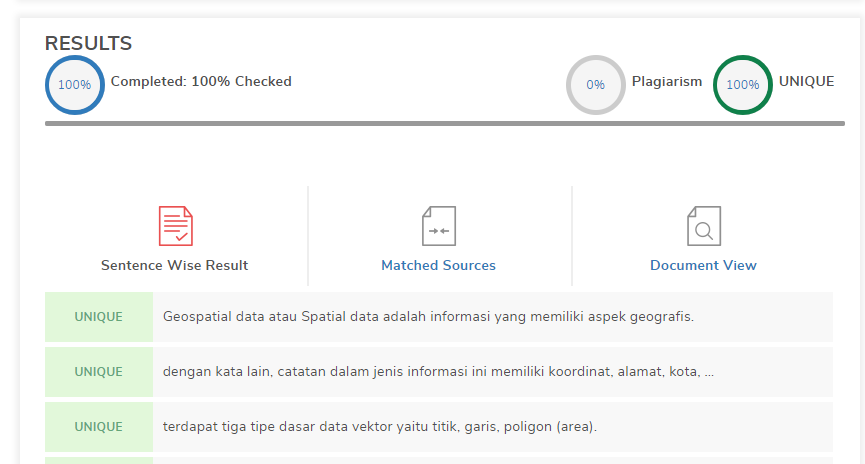
\includegraphics[width=8cm]{figures/Tugas1/1174091/plagiarisme.png}
	\centering
	\caption{Plagiarisme.}
\end{figure}	

\subsection{Cara Penggunaan}
\subsubsection{Gambar}

\hfill\break

Contoh Gambar
\begin{figure}[H]
	
\includegraphics[width=4cm]{figures/himatif.png}
	\centering
	\caption{Contoh gambar.}
\end{figure}

\subsubsection{List}
\begin{enumerate}
	\item Satu
	\item Dua
\end{enumerate}

\begin{itemize}
	\item Satu
	\item Dua
\end{itemize}



\section{Geographic Information System | Nurul Izza Hamka | 1174062}
\subsection{Buku}
Buku Belum Lunas
\subsection{Pengertian Sistem Informasi geografis}
\begin{enumerate}

\item Pemahaman Pada Sistem Informasi Geografis

Sistem Informasi Geografis merupakan pemahaman dari 3 rangkaian kata, sebagai berikut:\\
1. Geogarfi\\
Sistem Informasi Geografis dibangun berdasarkan pada istilah 'geografi' atau 'spasial'. Objek mengacu pada sfesifikasi  lokasi dalam suatu ruang/tempat. Objek dapat berupa fisik, budaya ataupun ekonomi alamiah.\\
2. Informasi\\
Informasi berasal dari kata pengelohan sejumlah data. Didalam sistem informasi geografis informasi mempunyai volume terbesar. Dan setiap object geografi memiliki setting datanya tersendiri karena tidak sepenuhnya data yang ada dapat terwakili di dalam peta. Maka, semua data harus diasosiasikan pada objek spasial yang mampu membuat peta menjadi intelligent.\\
3.Sistem\\
pengertian dari suatu sistem merupakan kumpulan elemen-elemen yang saling berintegrasi dan berinterdependensi dalam sebuah lingkungan yang dinamis untuk mencapai tujuan tertentu.\\

\item Definisi Sistem Informasi Geografis (Geographic Information System) 

Sistem informasi geografis adalah sebuah komputer yang berbasis sistem informasi yang digunakan untuk memberikan informasi bentuk digital dan analisa terhadap permukaan geografi bumi. \\
Sistem informasi geografis (GIS) diartikan sebagai sistem untuk penyimpanan, memerikas, mengintegrasi, memanipualasi, menganalisis dan memaparkan data yang berkaitan denagn semua ruang yang berhubungan dengan keadaan bumi.\\
Geografis adalah bidang kajian ilmu dan teknologi yang masih abru. Ada beberapa definisi dari Sistem Informasi Geograpis yaitu :\\
a. Definisi SIG menurut (Rhind, 1998) yaitu GIS is a computer system for collecting, integrating and analyzing information related to the surface of the earth.\\
b. Definisi SIG menurut (Marble dan Peuquet, 1983) and (Parker, 1988; Ozemoy et al.,1981; Burrough,1986) yaitu GIS deals with space-time data and often but notnecessarily, employs computer hardware and software)\\

\end{enumerate}
\subsection{Sejarah}
\begin{enumerate}
\item Peta\\
Peta merupakan penggambaran secara grafis atau bentuk skala (perbandingan) pada konsep mengenai bumi dalam hal ini peta merupakan alat untuk menyampaikan atau menginformasikan mengenai ilmu kebumian.\\
\item Peta Menurut Claudius Ptolemaeus Ptolemy\\
Claudius Ptolemaeus atau yang dikenal dengan nama Ptolemy (100 M dan 168 M), beliau merupakan salah satu sarjana sains pada masanya.Ptolemy membawa semua pengetahuan dan keterampilan matematika dan astronomi dan menerapkannnya pada pembuatan peta. Berdasarkan perhitungan  lingkara  dunia 18.000 mil, ia juga mengembankan sistem grid latude dan longitude yang dirancang oleh Marinus of Tire sementara beberapa rincian peta mungkin sedikit aneh dengan garis lintang sejajar dengan garis khatulistiwa dengan garis bujur yang membentang ke utara-selatan dengan busur anggun.\\
\item Peta Dunia Ptolemy\\
Peta duni ptolemy adalah gambaran dunia yang diketahui mesyarakat barat pada tahun kedua masehi. Peta tersebut berdasarkan penerangan yang terkandung di dalam buku Geographia, ditulis kira-kira pada 150 masehi walaupun peta autentik tidak dijumpai.\\
\end{enumerate}

\subsection{Koordinat}
\begin{enumerate}
\item Sistem Koordinat\\
\\
Dalam artikel Zuhdi menjelaskan Koordinat dimaksudkan untuk memberikan pengalamatan terhadapt setiap lokasi di permukaan  bumi. Pengalamatan dengan sistem koordinat didasarkan atas jarak timur-barat dan utara-selatan suatu tempat dari suatu titik pangkal tertentu. Jarak diukur dalam satuan derajat sudut yang dibentuk dari titik pengkal ke posisi tersebut melalui pusat bumi. Sedangkan titik pangkal ditetapkan berada di perpotongan belahan utara-selatan bumi (Khatulistiwa) dengan agris yang membela Bumi timur-barst melalui kota Greenwich di Inggris.\\
\end{enumerate}

\subsection{Data Geospasial}
\begin{enumerate}
\item Pengertian Geospasial\\
Informasi geospasial, yang lazim dikenal dengan peta, adalah informasi objek permukaan bumi yang mencakup aspek waktu dan keruangan. Pengertian Geo dalam geospasial, berarti geosfer yang mencakup atmosfer yang mencakup atmosfer lapisan udara yang meliputi permukaan bumi, pedosfer tanah beserta pembentukan dan zona-zonanya, sebagai bagian dari kulit bumi, hidrosfer lapisan air yang menutupi permukaan bumi dalam berbagai bentuknya, biosfer segenap unsur di permukaan bumi yang membuat kehidupan dan proses biotik  berlangsung dan antroposfer manusia dengan segala aktivitas yang di lakukannya di permukaan bumi.\\

\end{enumerate}
\subsection{Link}
https://youtu.be/InUXF34ojUc

\subsection{Plagiarism}
\begin{figure}[H]
	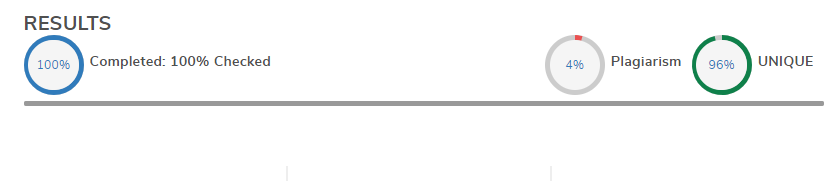
\includegraphics[width=4cm]{figures/Tugas1/1174062/plagiat.png}
	\centering
	\caption{Gambar Plagiat}
\end{figure}
\section{Ainul Filiani (1174073)}
\subsection{Buku}
Belum Lunas 
\subsection{Pengertian Sistem Informasi Geografis}
\begin{enumerate}
\item definisi sistem informasi geografis 
Sistem Informasi Geografis atau disingkat SIG (bahasa Inggris Sistem Informasi Geografis (SIG) adalah sebuah komputer yang berbasis sistem informasi yang digunakan untuk menyediakan informasi bentuk digital dan menganalisis terhadap permukaan geografi bumi. Sistem Informasi Geografis (SIG) diartikan sebagai sistem untuk menyimpan, memantau, mengintegrasi, memanipulasi, menganalisis dan memaparkan data yang berkaitan dengan semua ruang yang terkait dengan keadaan bumi. Artikel yang berasal dari Prahasta yang membahas tentang GIS adalah menyimpan, membaca, mengintegrasi, memanipulasi, menganalisis dan memaparkan data yang berkaitan dengan semua ruang yang berkaitan dengan keadaan bumi., Informasi dan Sistem 
[1] dan dalam artikel dari Husein dkk, yang menyebutkan bahwa Sistem Informasi Geografis merupakan pemahaman dari Geografi Informasi dan Sistem [2].
karena Sistem Informasi Geografis adalah bidang kajian ilmu dan teknologi yang masih baru. Beberapa resolusi dari Sistem Informasi Geografis yaitu:
Definisi SIG menurut (Rhind, 1988) yaitu GIS adalah sistem komputer untuk mengumpulkan, memeriksa, mengintegrasikan dan menganalisis informasi yang berkaitan dengan permukaan bumi. 
Definisi SIG menurut (Marble dan Peuquet, 1983) dan (Parker, 1988: Ozemoy et al., 1981; Burrough, 1986) yaitu GIS berkaitan dengan data ruang-waktu dan sering tetapi tidak selalu, mempekerjakan perangkat keras dan perangkat lunak komputer.
SIG adalah suatu sistem yang dapat mengupayakan perangkat keras (perangkat keras), perangkat perangkat lunak (perangkat lunak), dan data, serta dapat digunakan dan digunakan sistem penyimpanan, pengolahan, serta analisis data yang dilakukan secara simultan, sehingga dapat diperoleh seluruh informasi yang dimuat langsung dengan aspek ke dalam ruangan.  SIG adalah manajemen data spasial dan data non-spasial yang berbasis komputer dengan menggunakan tiga karakteristik dasar, yaitu: 
\end{enumerate}
\begin{enumerate}
\item Memiliki fenomena yang aktual (data variabel non-lokasi) dan terkait dengan topik topik di lokasi penelitian 
\item merupakan suatu lokasi Tertentu 
\item Memiliki dimensi waktu.  Alasan GIS diperlukan karena data spasial ditanganinya sangat sulit karena peta dan data cepatnya kadaluarsa sehingga tidak ada layanan penyediaan data dan informasi yang diberikan menjadi tidak akurat
\end{enumerate}
Berikut merupakan keistimewaan analisa dengan sistem informasi geografis:
\begin{enumerate}
\item analisa proximity
\item analisa overlay
\end{enumerate}
\subsection{Sejarah}
Peta merupakan penggambaran grafis atau bentuk skala (mempertimbangkan) pada konsep tentang bumi dalam hal ini peta merupakan alat untuk melengkapi atau memuat tentang ilmu kebumian.  Bagaimana peta dahulu ditemukan?  Pengetahuan tentang dasar pembentukan sama seperti filsafat, yang mana sering dianggap berbeda.  Peta Menurut Claudius Ptolemaeus Ptolemy, Claudius Ptolemaeus yang dikenal dengan nama Ptolemy, hidup antara tahun 100 M dan 168 M, beliau merupakan salah satu sarjana sains pada masanya.  Dia tinggal dan bekerja di Alexandria, kota Mesir yang merupakan pusat Intelektual dunia barat dengan perpustakaan paling luas yang pernah diciptakan.  Ptolemy membawa semua pengetahuan dan keterampilan matematika dan astronomi dan menerapkannya pada pembuatan peta.  Dia memiliki daya tarik matematikawan dengan presisi untuk menunjukkan hubungan satu tempat ke tempat lain.  Berdasarkan perhitungan lingkaran dunia 18.000 mil, ia juga mengembangkan sistem grid latude dan bujur yang dirancang olehMarinus dari Tirus sementara beberapa rincian peta mungkin sedikit aneh dengan garis lintang sejajar dengan garis khatulistiwa dengan garis bujur yang membentang ke utara-selatan dengan busur anggun, sudah tidak tersedia  lagi bagi siapa saja yang pernah memiliki atlas.  Dalam persetujuan ini, Ptolemeus dapat membangun koordinat dan meminta lebih dari 8000 tempat koordinat masing-masing Bagi Ptolemeus, ini latihan matematik dan kita tidak akan pernah tahu apakah dia benar-benar membuat peta dari sini.
\subsection{koordinat}
Koordinat digunakan untuk menentukan titik di Bumi melalui garis lintang dan garis bujur.  Koordinat dibagi menjadi dua bagian irisan yaitu irisan melintang yang disebut dengan garis lintang mulai dari khatulistiwa, membesar ke arah kutub (utara maupun selatan) sedangkan yang lain membujur mulai dari garis Greenwhich membesar ke arah barat dan timur.  Koordinat ini ditulis dalam satuan derajat, menit, dan detik dan seterusnya. Untuk membagi dunia di dalam wilayah utara dan selatan, maka ditentukan garis yang tepat berada di tengah, yaitu garis Khatulistiwa atau Khatulistiwa. Untuk batas wilayah timur dan  barat, maka ditentukan sebuah garis Perdana meridian yang terletak di kota Greenwich (Inggris), dan perpotongannya bertemu di wilayah laut pasifik, yaitu memotong kepulauan Fiji.
\begin{itemize}

\item Garis Lintang 
Sebuah garis khayal yang digunakan untuk menentukan lokasi di Bumi terhadap garis khatulistiwa (utara atau selatan).  Posisi lintang merupakan penghitungan sudut dari 0 derajat di khatulistiwa sampai ke +90 derajat di kutub utara dan -90 derajat di kutub selatan.  Dalam bahasa Indonesia lintang di sebelah utara khatulistiwa diberi nama Lintang Utara (LU), demikian pula lintang di sebelah selatan khatulistiwa diberi nama Lintang Selatan (LS).  Lintang Utara dan Lintang Selatan menentukan sudut pandang antara posisi lintang dengan garis Khatulistiwa.  Garis Khatulistiwa sendiri adalah lintang 0 derajat.  Nilai koordinat lintang dimulai dari garis lingkaran khatulistiwa yang diberi nilai 0 derajat.  Selanjutnya garis lintang yang lain berbentuk lingkaran paralel (sejajar) khatulistiwa berada di sebelah utara dan selatan khatulistiwa.  Lingkaran paralel di selatan disebut garis lintang selatan (LS) dan diberi nilai negatif, sedangkan lingkaran paralel di utara diberi nilai positif dan disebut garis lintang utara.
\item Garis Bujur
Menggambarkan lokasi tempat di timur atau barat Bumi dari garis utara-selatan yang disebut Meridian Utama.  Bujur diberikan pada sudut pandang yang terdiri dari 0 derajat Meridian Utama ke +180 derajat Arah timur dan-180 derajat Arah barat Tidak seperti lintang yang memiliki ekuator sebagai posisi awal yang tidak memiliki posisi awal yang alami untuk perbatasan.  Bujur di sebelah barat Meridian diberi nama Bujur Barat (BB), demikian pula bujur di sebelah timur Meridian diberi nama Bujur Timur (BT).  Nilai koordinat garis bujur dimulai dari bujur 0 derajat yaitu Greenwhich, kemudian diperbesar ke arah timur dan barat sampai bertemu kembali di garis batas tanggal internasional yaitu terletak di selat bering dengan nilai 180 derajat.  Garis bujur 0 derajat disebut prime meridian atau meridian Greenwhich.  Garis bujur ke arah barat diberi nilai negatif dan disebut bujur barat (bujur barat) serta disingkat BB.  Sedangkan garis bujur yang ke arah timur diberi nilai positif dan disebut bujur timur (bujur timur) disingkat BT.  nilai koordinat atas yang disusun dari bujur 0 ke atas sesuai dengan pusat bumi.
\end{itemize}
\subsection{Data geospasial}
data raster adalah data yang tersimpan dalam bentuk grid atau petak jadi terbentuk pada sebuah ruang yang teratur dalam bentuk pixel (elemen gambar).  Foto digital seperti areal fotografi atau satelit merupakan bagian dari data raster pada peta.  Data raster memiliki kisi-kisi data terus. Diharapkan menggunakan gambar berwarna seperti fotografi, yang disetujui dengan tingkat merah, hijau, dan biru pada sel.  Data Raster (atau disebut juga dengan sel grid) merupakan data yang dihasilkan dari sistem penginderaan jauh.  Pada data raster.  Obyek geografis direpresentasikan sebagai struktur sel grid yang disebut dengan pixel (elemen gambar).  Pada data raster.  Resolusi (resolusi visual) tergantung pada ukuran pixelnya.  Dengan kata lain.  Resolusi piksel. Resolusi setiap kali bumi diwakili oleh setiap piksel pada citra.  Pada data raster, objek arsitektur direpresentasikan sebagai struktur sel grid yang disebut se-bagi pixel (elemen gambar).  Resolusi (resolusi visual) tergantung pada ukuran pixel-nya, semakin kecil ukuran permukaan bumi yang direpresentasikan oleh sel, semakin tinggi resolusinya.  Data Raster dihasilkan dari sistem penginderaan jauh dan sangat baik untuk merepresentasikan batas-batas yang berubah secara bertahap seperti jenis tanah, kelembaban tanah, suhu, dan lain-lain.
\subsection{link}
https://youtu.be/VtkOzHAdmk0
\subsection{plagiarisme}
\begin{figure}[H]
 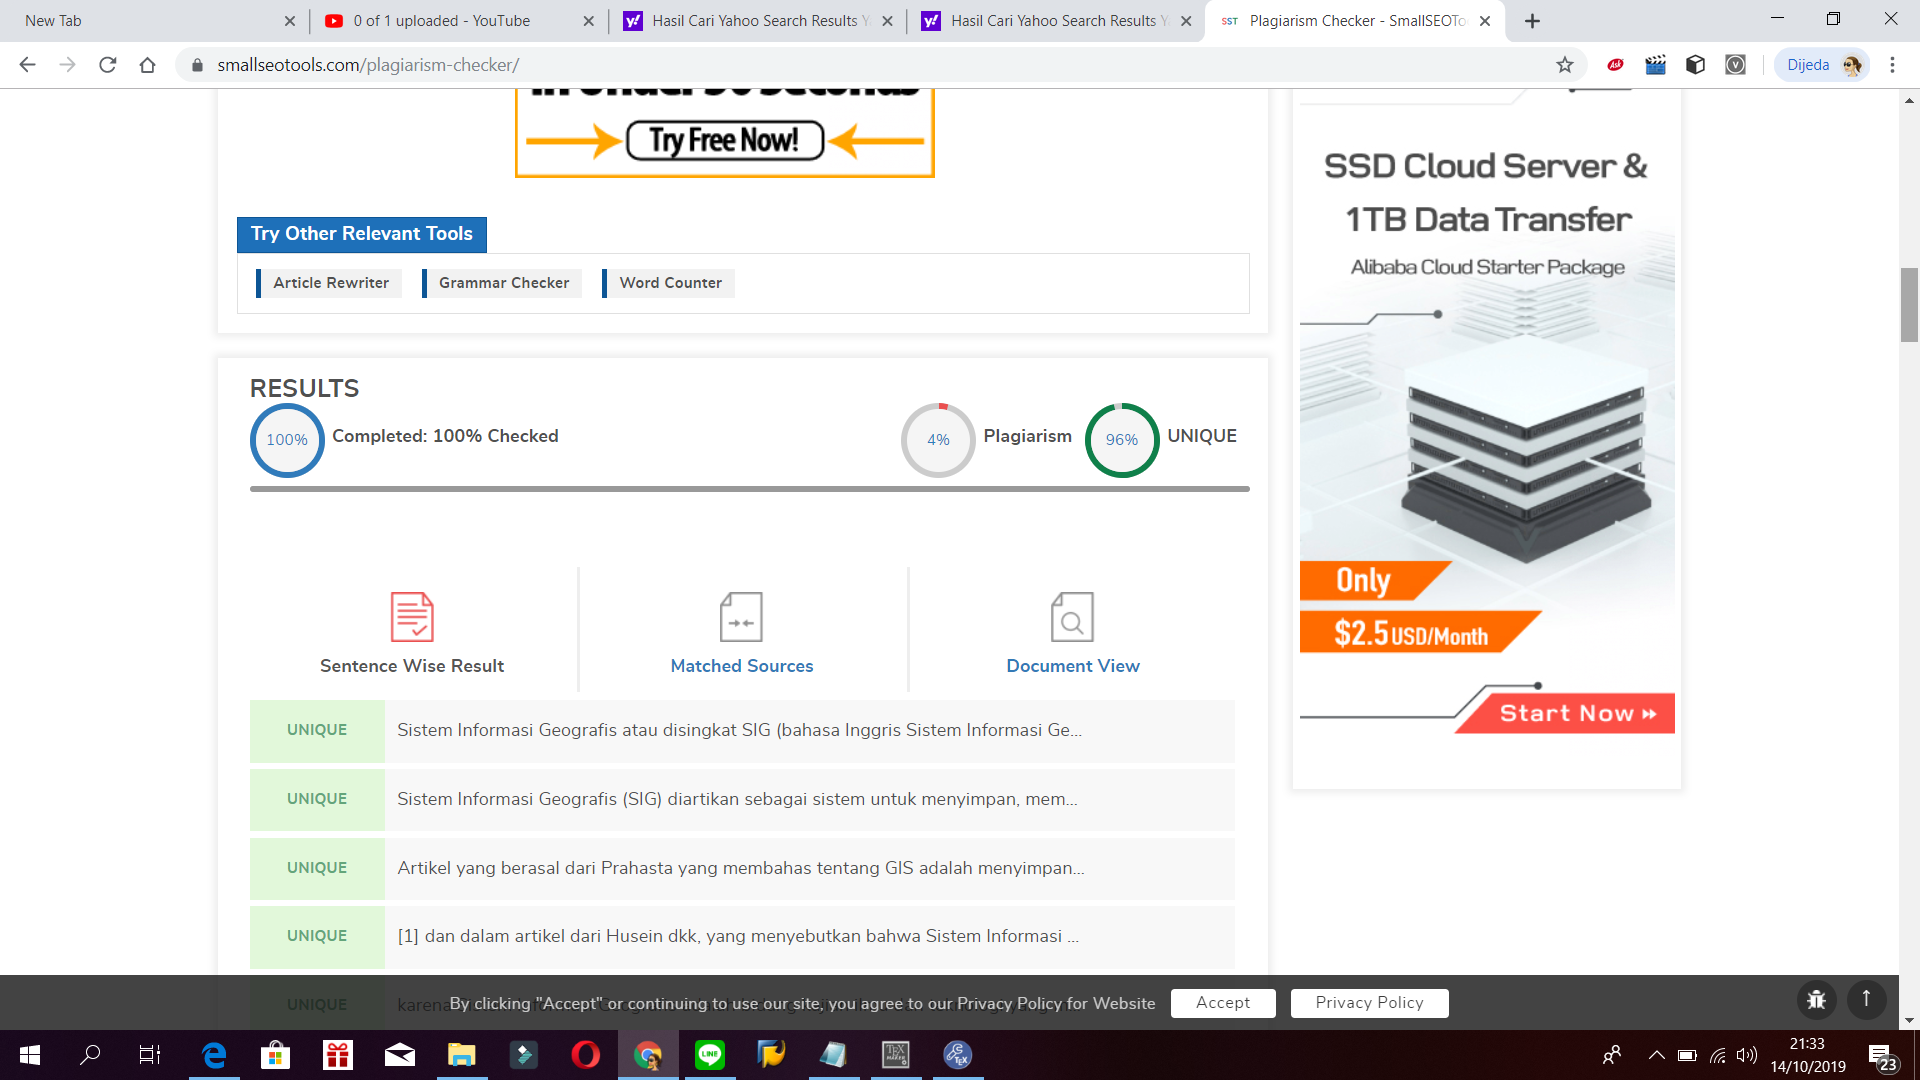
\includegraphics[width=4cm]{figures/Tugas1/1174073/plagiarism.png}
 \centering
 \caption{Gambar Plagiat}
\end{figure}
\section{Aulyardha Anindita | 1174054}
\subsection{Buku}
Belum Lunas
\subsection{Sistem Informasi Geografis}
\paragraph{}
Sistem Informasi Geografis atau disingkat SIG (bahasa Inggris: Geographic Information System (GIS)) adalah sebuah komputer yang berbasis sistem informasi yang digunakan untuk memberikan informasi bentuk digital dan analisa terhadap permukaan geografi bumi.

Sistem Informasi Geografis (GIS) diartikan sebagai sistem untuk menyimpan, memeriksa, mengintegrasi, memanipulasi, menganalisis dan memaparkan data yang berkaitan dengan semua ruang yang berhubungan dengan keadaan bumi.

Definisi dari Sistem Informasi Geografis dapat selalu berubah karena Sistem Informasi Geografis adalah bidang kajian ilmu dan teknologi yang masih baru. beberapa definisi dari Sistem Informasi Geografis yaitu :
\begin{enumerate}
\item Menurut Rhind (1988), GIS is a computer system for collecting, checking, integrating and analyzing information related to the surface of the earth.
\item Menurut Marble and Puequet (1983) and Parker (1988) yaitu GIS deals with space-time data and often but not necessarily, employs computer hardware and software.
\end{enumerate}

Sistem Informasi Geografis merupakan gabungan dari 3 kata, yaitu Sistem, Informasi dan Geografis
\begin{enumerate}
\item Geografi, yaitu objek yang mengacu pada spesifikasi lokasi dalam suatu tempat/ruang. objek dapat berupa fisik,budaya ataupun ekonomi alamiah.
\item Informasi, berasal dari kata pengolahan sejumlah data. Didalam GIS informasi mempunyai volume besar. Dan setiap objek geografi memiliki setting datanya tersendiri karena tidak sepenuhnya data yang ada dapat terwakili didalam peta.
\item Sistem, yaitu kumpulan elemen-elemen yang saling beritegrasi dan berinterdependensi dalam sebuah lingkungan yang dinamis untuk mencapai tujuan tertentu.
\end{enumerate}

\subsection{Sejarah}
\paragraph{}
Peta merupakan penggambaran secara grafis atau bentuk skala (perbandingan) pada konsep mengenai bumi dalam hal ini peta merupakan alat untuk menyampaikan atau menginformasikan mengenai ilmu kebumian.

Sejarah Peta dapat dikelompokkan berdasarkan perkembangannya yaitu sebagai berikut :
\begin{enumerate}
\item Peta Ptolemy
\paragraph{}
Claudius Ptolemaeus yang dikenal dengan nama Ptolemy, hidup antara tahun 100 M dan 168 M, beliau merupakan salah satu sarjana sains pada masanya. Ptolemy membawa semua pengetahuan dan keterampilan matematika dan astronomi dan menerapkannya pada pembuatan peta. Ptolemy mampu membangun koordinat dan mendaftarkan lebih dari 8000 tempat dengan koordinat masing-masing. 

Geografi ptolemy diterjemahkan dalam bahasa latin dan gagasannya terhadap PETA Dunia dapat diakses oleh para ilmuwan, namun tidak ada peta dalam keadaan utuh, hanya petunjuk dan saran untuk pembuatan map dan daftar koordinat.

Peta dunia Ptelomy adalah peta gambaran dunia yang diketahui masyarakat barat pada kurun kedua masehi. Peta tersebut berdasarkan penerangan yang terkandung didalam buku Geographia, ditulis kira-kira pada 150 masehi walaupun peta autentik tidak dijumpai, buku Geographia yang berisi beribu-ribu rujukan dari berbagai tempat didunia, beserta koordinat, yang membolehkan para pelukis peta menyusun semula peta dunia Ptolemy apabila manuskripnya telah ditemui sekitar 1300 masehi.

Peta di manuskrip yang masih ada di Ptolemy's Geography yang berasal sekitar tahun 1300 yang ditemukan kembali oleh Maximus Planudes. Pada abad ke-15, Geografi Ptelomy mulai dicetak dengan peta terukir, edisi cetak paling awal dengan peta terukir diproduksi di Bologna pada 1477, diikuti dengan cepat oleh edisi Romawi tahun 1478.

Ptolemy memperkirakan ukuran bumi terlalu kecil, sementara Eratosthones menemukan 700 stadion untuk sebuah lingkaran besar didunia, Ptolemy menggunakan 500 stadion di geografi. Sangat mungkin bahwa ini adalah stadion yang sama, karena Ptolemy beralih dari skala sebelumnya ke yang terakhir antara Syntaxis dan Geography, dan menyesuaikan derajat bujur yang sesuai.

Karena Ptolemy berasal dari garis lintang utamanya dari nilai terpanjang minyak mentah, garis lintangnya rata-rata keliru kira-kira satu derajat (2 derajat Byzantium, 4 derajat Kartago), meskipun para astronom kuno mampu mengetahui garis lintang mereka lebih lama.

\item Erathosthenes\\
Erathosthenes adalah salah satu tokoh ilmiah paling terkemuka di masanya, dan menghasilkan karya-karya yang mencakup pengetahuan luas sebelum dan selama waktunya di Perpustakaan.

Lebih dari 2000 tahun yang lalu Erathosthenes membandingkan posisi matahari di dua lokasi untuk menentukan ukuran bumi dengan alasan yang akurat. Dengan menggunakan penemuan dan pengetahuan tentang ukuran dan bentuknya, dia mulai membuat sketsa.

Dalam karya jilid tiganya Geografi, dia menggamabrkan dan memetakan seluruh dunia yang dikenalnya,bahkan membagi bumi menjadi lima zona iklim yaitu dua zona pembekuan disekitar kutub, dua zona beiklim sedang, dan sebuah zona yang meliputi khatulistiwa dan daerah tropis. Dia menciptakan geografi yang masih digunakan sampai sekarang.

Pencapaian Eratosthenes yang paling abadi adalah perhitungan lingkar bumi yang sangat akurat. Dia menghitung ini dengan menggunakan geometri dan trigonometri sederhana dan dengan mengenali bumi sebagai bola di ruang angkasa.

Eratosthenes bisa mengukur sudut sinar matahari dari vertikal dengan membagi panjang kaki diseberang sudut (panjang bayangan) dengan kaki yang bersebelahan dengan sudut (tinggi tiang). Ini memberinya sudut 7,16 derajat. Dia tahu bahwa lingkar bumi membentuk lingkaran 360 derajat, jadi 7,12 derajatnya dikira-kira seperlima puluh keliling. Dia juga tahu perkiraan jarak antara Alexandria dan Syene, jadi dia bisa mengatur persamaan ini.

\item Peta Al Idrisi\\
Pada Abad ke-12, geografer Al Idrisi berhasil membuat peta dunia. Al Idrisi yang lahir pada tahun 1100 di Ceuta Spanyol juga menulis kitab geografi yang berjudul Kitab Nazhah Al Muslak fi Ikhtira Al Falak. Kitab ini begitu berpengaruh sehingga diterjemahkan kedalam bahasa latin, Geographia Nubiensis. Seabad kemudian, dua geografir yakni Qutubuddin Asy Syirazi (1236 M-1311 M) dan Yaqut Ar Rumi (1179 M-1129 M) berhasil melakukan terobosan baru.

Qutubuddin mampu membuat peta laut putih atau laut tengah yang dihadiahkan kepada raja persia. Sedangkan, yaqut berhasil menulis enam jilid ensiklopedia bertajuk Mujam Al Budan. Sederet geografer telah banyak memberi kontribusi bagi pengembangan ilmu bumi. Al Kindi begitu diakui berjasa sebagai geografer pertama yang memperkenalkan percobaan ke dalam ilmu bumi.

Pada periode yang sama, Willem Jansz Blaeu dianggap menerbitkan peta dinding dunia dengan proyeksi stereografik. Peta dinding diterbitkan pada tahun 1605 oleh Willem Jansz Blaeu dan pada akhirnya untuk memenuhi semua kebutuhan pelanggannya, Willem memutuskan untuk menerbitkan peta dunia mengenai proyeksi Mercator. Peta dinding ini diproyeksikan akan berpengaruh pada peta dunia lainnya, tidak ada salinan lengkap dari peta ini yang bertahan.
\end{enumerate}

\subsection{Koordinat Bumi}
Menurut sebuah artikel dari Mohd Zuhdi menyebutkan bahwa sistem koordinat dimaksudkan untuk memberikan pengalamatan terhadap setiap lokasi di permukaan bumi. Pengalamatan dengan sistem koordinat didasarkan atas jarak timur sampai dengan barat dan utara sampai dengan selatan suatu tempat dari suatu titik pangkal tertentu. Jarak diukur dalam satuan derajat dengan sudut yang dibentuk dari titik pangkal ditetapkan yang berada di perpotongan belahan utara sampai dengan selatan bumi (garis khatulistiwa) dengan garis yang membelah bumi bagian timur sampai dengan barat melewati kota Greenwhich di Inggris.

Posisi suatu tempat dialamatkan dengan nilai koordinat garis bujur (longitude) dan lintang (latitude) yang melalui tempat itu. Garis bujur biasanya juga disebut sebagai garis median, yaitu merupakan garis lurus yang menyambungkan dari kutub utara sampai selatan bumi. Nilai koordinat garis bujur ini dimulai dari bujur 0 derajat yaitu di Greenwich, kemudian membesar ke arah timur dan barat sampai bertemu kembali di garis batas internasional yaitu terletak di Selat Bering dengan nilai 180 derajat.

Garis bujur 0 derajat sering disebut prime meridian atau meridian Greenwich,garis bujur ke arah barat diberi nilai negatif dan disbeut bujur barat serta disingkat BB. sedangkan garis bujur yang kearah timur diberi nilai positif dan disebut bujur timur disingkat BT. Nilai koordinatnya didasarkan atas besarnya sudut yang terbentuk dari bujur 0 ke garis bujur tersebut melalui pusat bumi.

Adapun nilai koordinat lintang dimulai dari garis lingkaran khatulistiwa yang diberi nilai 0 derajat. Selnajutnya garis-garis lintang yang lain berupa lingkaran paralel (sejajar) khatulistiwa berada disebelah utara dan selatan khatulistiwa. Lingkaran paralel diselatan disebut garis lintang selatan (LS) dan diberi nilai negatif, sedangkan lingkaran paralel di utara diberi nilai positif dan disebut garis lintang utara (LU). Nilai maksimum koordinat garis lintang adalah 90 derajat yaitu terletak di kutub-kutub bumi.

\subsection{Data Geospasial}
Geospasial terdiri dari dua kata, yaitu geo dan spasial. geo berarti bumi sedangkan spasial berarti ruang. UU No.4 Tahun 2011 tentang geospasial menyebutkan, spasial adalah aspek keruangan dari suatu objek, atau mencakup lokasi, letak dan posisinya. Data Geospasial dipecah menjadi dua yaitu yang pertama Data Grafis atau geometri. Data ini terdiri dari tiga elemen yaitu titik, garis, dan luasan. Data ini berbentuk vektor maupun raster. Kedua data tersebut adalah data atribut atau data tematik.

Ada beberapa jenis Data Geospasial yaitu:
\begin{enumerate}
\item Data Raster \\
Data Raster adalah data yang disimpan dalam bentuk grid atau petak sehingga terbentuk suatu ruang yang teratur dalam bentuk pixel (picture element). Data raster memiliki data grid continue.Foto digital seperti areal fotografi atau satelit merupakan bagian dari data raster pada peta.
\item Data Vektor \\
Data Vektor adalah data yang direkam dalam bentuk koordinat titik yang menampilkan, menempatkan dan menyimpan data spasial dengan menggunakan titik,garis, atau are (polygon).
\item Data Line
Data Line merupakan bentuk geometri linear yang menghubungkan dua titik atau lebih dan biasanya digunakan untuk merepresentasikan objek berdimensi satu. Garis bisa digunakan untuk menunjukkan route suatu perjalanan atau menggambarkan boundary

\end{enumerate}

\subsection{Link Youtube}
https://youtu.be/Yu4bFe3GxHQ

\subsection{Plagiarisme}
\begin{figure}[H]
	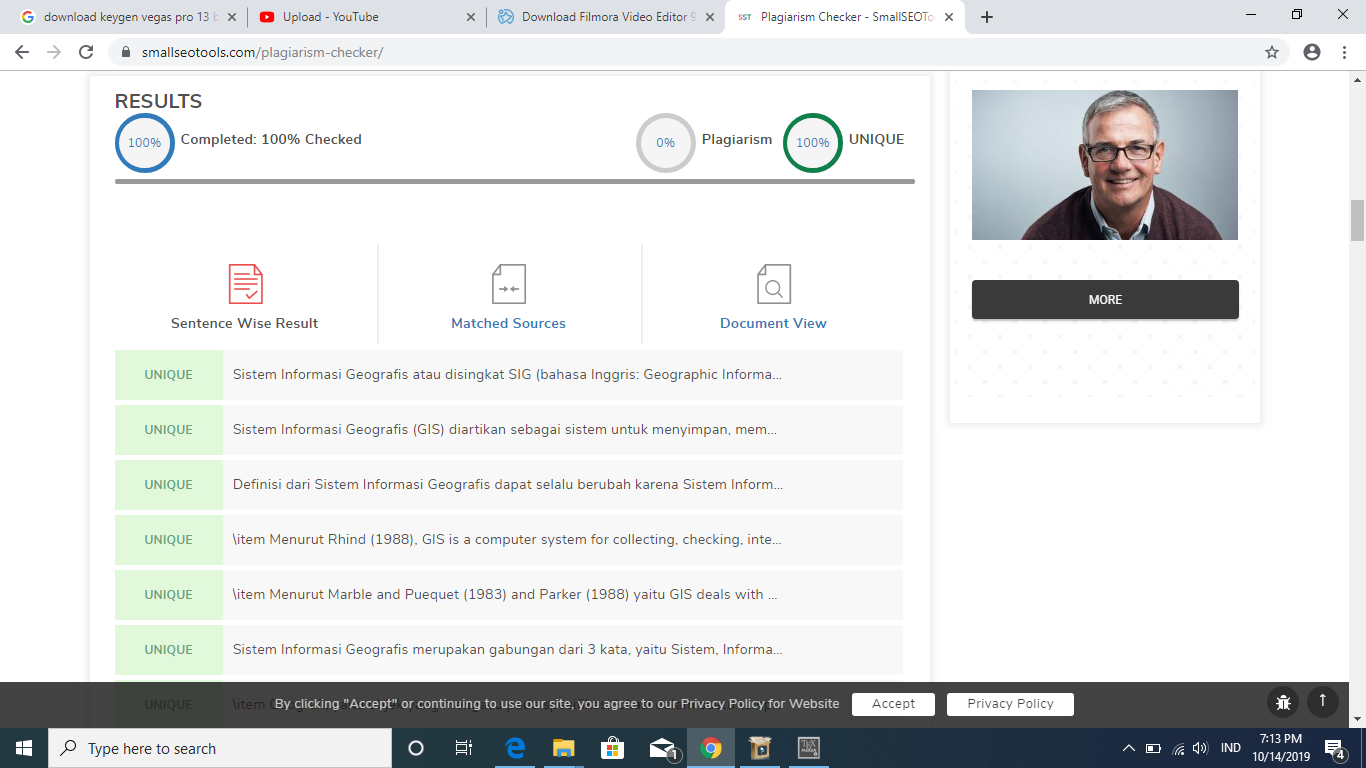
\includegraphics[width=4cm]{figures/Tugas1/1174054/plagiarismetgas1.png}
	\centering
	\caption{Gambar Plagiarisme}
\end{figure}
\section{Difa Al Fansha(1174076)}
\subsection{Pengertian}
\begin{itemize}
	\item \textbf{Geografi} \\
	'Merupakan ilmu yang melukiskan dan menggambarkan keadaan bumi.' \\ 
(Erastoshenes, 200SM). \\ 
Geografi biasa disebut juga dengan spasial, geografi sangat berkaitan dengan peta, karena peta adalah gambaran sebuah lingkungan. Dalam peta, simbol, warna dan gaya garis digunakan sebagai perwakilan dari setiap spasial yang berbeda pada peta poligon (2-D) dan permukaan (3-D)
	
	\item \textbf{Informasi} \\
Pengolahan sejumlah data (gambar, suara, text, dan lain sebagainya). Semua data harus diasosiasikan pada object spasial yang mampu mmebuat peta menjadi cerdas (intelligent).

	\item \textbf{Sistem} \\
Kumpulan elemen-elemen yang saling  berhubungan dalam sebuah lingkungan yang dinamis untuk mencapai tujuan tertentu.
	
	\item \textbf{Kesimpulan :} \\
Sistem geografi adalah sebuah komputer yang berbasis sistem informasi digunakan untuk memberikan informasi bentuk digital dan analisa terhadap permukaan georafi bumi.\\
Definisi dari sistem informasi geografis dapat selalu berubah-ubah, karna sig merupakan bidang kajian ilmu dan teknologi yang masih baru.

\end{itemize}

\subsection{Link}
https://youtu.be/2SusnHVlTYA

\subsection{Plagiarism}
\begin{figure}[H]
	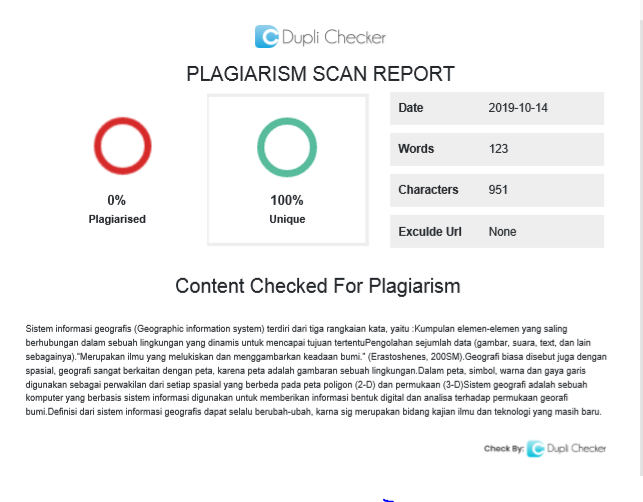
\includegraphics[width=8cm, height=8cm]{figures/Tugas1/1174076/1174076.png}
	\centering
	\caption{Gambar Plagiarisme 1174076}
\end{figure}
\section{Mochamad Arifqi Ramadhan (1174074)}
\subsection{Kordinat}
\begin{itemize}
	\item Pengertian Kordinat
	kordinat pada pemetaan adalah pertemuan antara garis bujur (Garis garis lurus atau vertikal pada peta) dan garis lintang (Garis mendatar atau horizontal pada peta). Artinya dalam peta kita akan menemukan garis melintang dan mebujur yang membagi peta menjadi kotak-kotak persegi.
Garis yang melintang dari kiri ke kanan peta disebut Garis Lintang (Latitude), sedangkan garis yang membujur dari atas ke bawah peta disebut Garis Bujur (Longitude).
Bersama, Garis Lintang dan Garis Bujur membentuk sistem koordinat peta.

Garis Lintang digunakan untuk menandai posisi utara-selatan sebuah lokasi di permukaan bumi. Garis Lintang berkisar dari 0 derajat di khatulistiwa sampai 90 derajat Lintang Utara di Kutub Utara dan 90 derajat Lintang Selatan di kutub Selatan.

Sementara itu Garis Bujur digunakan untuk menandai posisi utara-selatan sebuah lokasi di permukaan bumi. Garis Bujur 0 derajat terletak di kota Greenwich, Inggris, dan bergerak sejauh 180 derajat ke barat dan timur, yang bertemu pada titik 180 derajat di tengah Samudera Pasifik. Jarak antara masing-masing derajat garis lintang kira-kira 69 mil (111 km).

Contoh koordinat dengan Garis Lintang dan Garis Bujur ini adalah kota Jakarta dengan lokasi terletak di 6,2 derajat Lintang Selatan dan 107 derajat Bujur Timur.

\item Sejarah Kordinat
	
Konsep sudut dan jari-jari sudah digunakan oleh manusia sejak zaman purba, paling tidak pada milenium pertama SM. Astronom dan astrolog Yunani, Hipparchus, (190–120 SM) menciptakan tabel fungsi chord dengan menyatakan panjang chord bagi setiap sudut, dan ada rujukan mengenai penggunaan koordinat polar olehnya untuk menentukan posisi bintang-bintang.[2] Dalam karyanya On Spirals, Archimedes menyatakan Archimedean spiral, suatu fungsi yang jari-jarinya tergantung dari sudut. Namun, karya-karya Yunani tidak berkembang sampai ke suatu sistem koordinat sepenuhnya.

Dari abad ke-8 M dan seterusnya, para astronom mengembangkan metode untuk menghitung arah ke Mekkah (kiblat)— dan jaraknya — dari semua lokasi di bumi

	\item Sistem Kordinat 
Sistem kordinat merupakan suatu parameter yang menunjukkan bagaimana suatu objek diletakkan dalam koordinat. Ada 3 sistem kordinat yang digunakan dalam pemetaan, antara lain :


	\begin{enumerate}
	\item Sistem Koordinat 1 Dimensi
	
	\begin{figure}[H]
	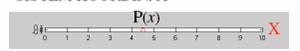
\includegraphics[width=4cm]{figures/Tugas1/1174074/dimensi1.jpg}
	\centering
	\caption{Gambar 1}
\end{figure}
	
	\item Sistem Koordinat 2 Dimensi 

	\begin{figure}[H]
	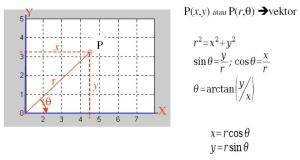
\includegraphics[width=4cm]{figures/Tugas1/1174074/dimensi2.jpg}
	\centering
	\caption{Gambar 1}
\end{figure}

\item Sistem Koordinat 3 Dimensi

	\begin{figure}[H]
	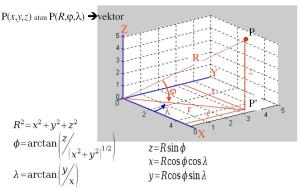
\includegraphics[width=4cm]{figures/Tugas1/1174074/dimensi3.jpg}
	\centering
	\caption{Gambar 1}
\end{figure}

	\end{enumerate}
\end{itemize}
\subsection{Link}
https://youtu.be/5nS7ewD8DQU
\subsection{Plagiarism}
\begin{figure}[H]
	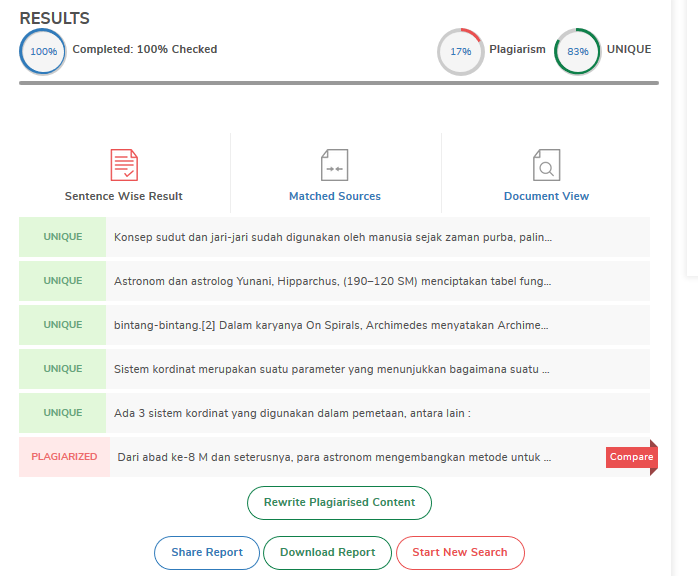
\includegraphics[width=4cm]{figures/Tugas1/1174074/plagiat.png}
	\centering
	\caption{Gambar Plagiat}
\end{figure}

	

\section{Muhammadd Abdul Gani Wijaya 1174071}
\subsection{DATA GEOSPASIAL} 
Geospasial terdiri dari dua kata, yaitu geo dan spasial. Geo berarti bumi dan spasial berarti ruang. Data geospasial adalah aspek keruangan dari suatu objek, atau yang mencakup lokasi, letak, dan posisinya. Data geospasial dipecah menjadi dua, yaitu data grafis/geometris dan data atribut/tematik. Data grafis adalah data yang terdiri dari tiga elemen yaitu titik, garis, dan luasan yang berbentuk vector maupun raster. Yang kedua adalah data atribut atau data tematik.
\begin{figure}[!htbp]
\centering
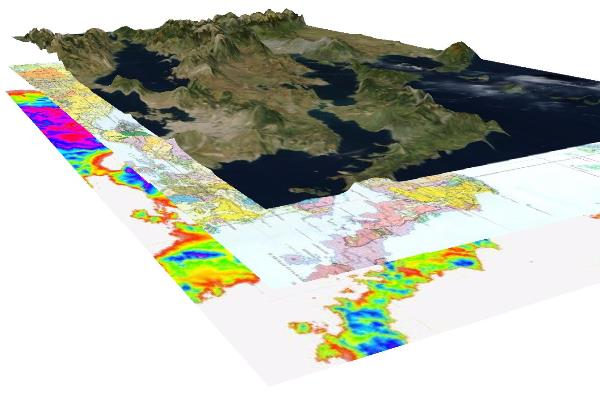
\includegraphics[width=6cm,height=6cm]{figures/Tugas1/1174071/Geospasial.jpg}
\caption{Data Geospasial}
\end{figure}	
\subsection{DATA GEOSPASIAL RASTER}
Data raster adalah data yang disimpan dalam bentuk grid atau petak sehingga terbentuk suatu ruang yang teratur dalam bentuk pixel (picture element). Foto digital seperti areal fotografi atau satelit merupakan bagian dari data raster pada peta.
\begin{figure}[!htbp]
\centering
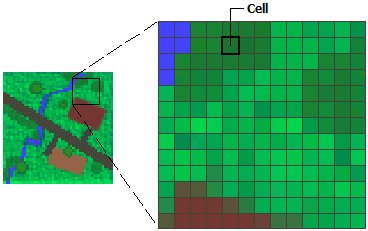
\includegraphics[width=6cm,height=6cm]{figures/Tugas1/1174071/Raster.png}
\caption{Data Raster}
\end{figure}	
\subsection{DATA GEOSPASIAL VEKTOR}
Data vector adalah data yang disimpan dalam bentuk koordinat titik yang menampilkan, menempatkan, dan menyimpan data spasial dengan menggunakan titik, garis, atau polygon. Terdapat tiga jenis data vector yaitu titik, garis, dan polygon. Tipe data ini biasanya terdapat pada peta. Setiap bagian dari data vector bias saja mempunyai informasi yang berasolasi satu sama lain.
\begin{figure}[!htbp]
\centering
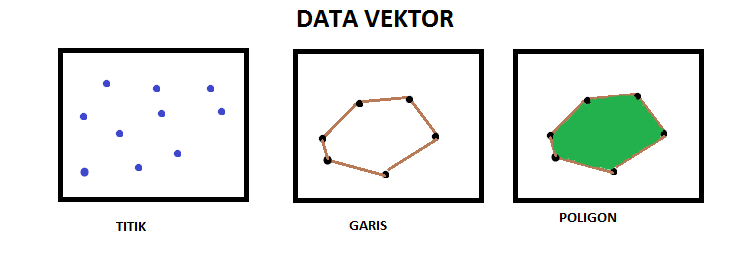
\includegraphics[width=6cm,height=6cm]{figures/Tugas1/1174071/Vektor.PNG}
\caption{Data Vektor}
\end{figure}	
\subsection {DATA GEOSPASIAL (OPEN GEOSPASIAL CONSORTIUM)}
Open Geospasial Consortium (OGC) Web Services (OWS) adalah layanan yang didefinisikan oleh OGC, yang memungkinkan semua jenis fungsi geospasial. Layanan yang ada pad OGC ini termasuk layanan untuk akses data, tampilan data dan pengolahan data. Permintaan OWS didefinisikan dengan menggunakan protocol Hyper Text Transfer Protocol (HTTP) dan dikodekan menggunakan struktur keyvaluepair (KVP) atau Exentible Markuo Language (XML). OWS yang paling banyak dikenal adalah Web Map Services (WMS).
\begin{figure}[!htbp]
\centering
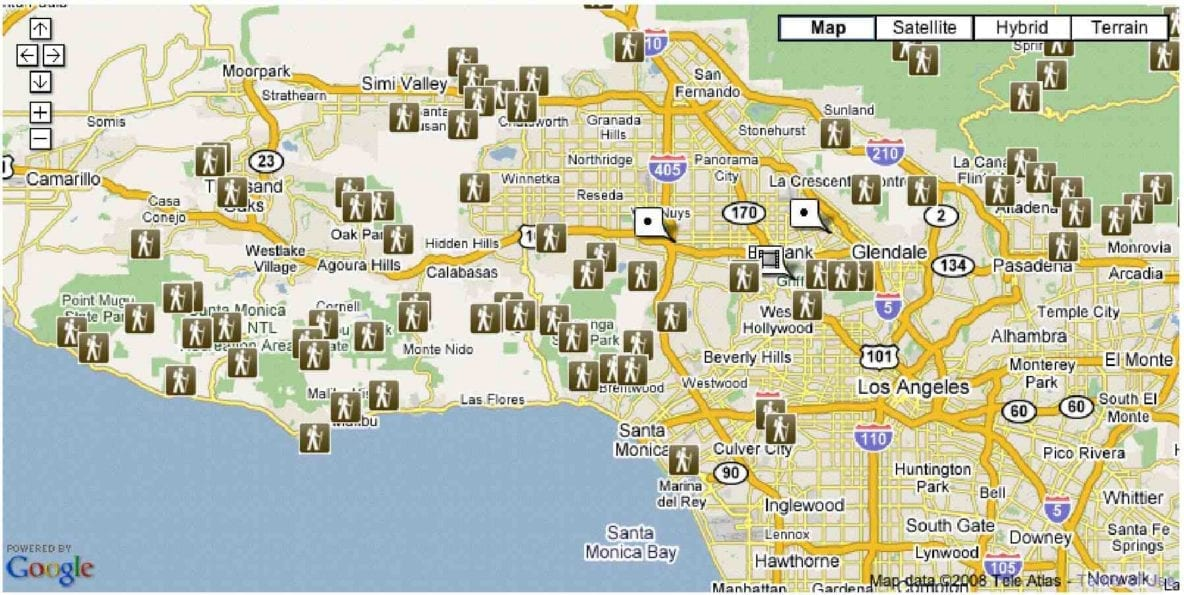
\includegraphics[width=6cm,height=6cm]{figures/Tugas1/1174071/OGC.jpg}
\caption{Open Geospasial Consortium}
\end{figure}
\subsection {Link Youtube}
https://youtu.be/unKOdRU1z4E
\subsection {Check Plagiarism}
\begin{figure}
\centering
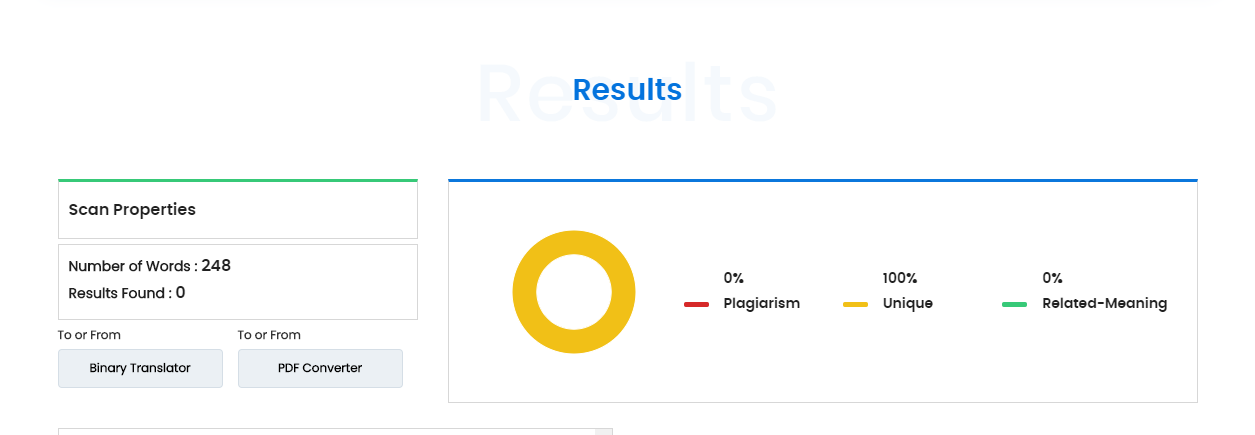
\includegraphics[width=15cm,height=10cm]{figures/Tugas1/1174071/Plagiarism.png}
\caption{Check Plagiarism}
\end{figure}
\section{Handi Hermawan (1174067)}
\subsection{Definisi}
\begin{enumerate}
	\item Geographic information system (GIS) adalah sebuah komputer yang berbasis sistem iformasi digunakan untuk memberikan informasi dalam bentuk digital dan analisa terhadap geografi bumi
	\item Sistem informasi geografis diartikan sebagai sistem untuk menyimpan, memeriksa, mengintegrasi, memanipulasi, mengananlisis dan memaparkan data yang berkaitan dengan keadaan bumi.
	\item GIS adalah manajemen data spasial dan non-spasial yang berbasis komputer dengan menggunakan  tiga karakteristik dasar, yaitu fenomena yang aktual, merupakan kejadian disuatu lokasi tertentu, memiliki dimensi waktu.
	
	\item Ada keistimewaan menganalisa menggunakan sistem informasi geografis yaitu :
\end{enumerate}
	\begin{itemize}
	\item Analisa Proximity adalah geografi yang berbasis pada jarak antar layer
	\item Analisa Overlay adalah proses integrasi data dari lapisan layer yang berbeda (overlay) yang secara analisa membutuhkan lebih dari satu layer.
    \end{itemize}
    
\subsection{Pemahaman GIS}
Geografi objeknya mengacu pada spesifikasi dalam suatu tempat atau ruang. Dimana simbol, warna dan gaya garis digunakan sebagai perwakilan dari setiap spasial yang berbeda pada peta dua dimensi berupa :
    \begin{itemize}
	\item Format titik
	\item Format Garis 
	\item Format Poligon 
	\item Format Permukaan
    \end{itemize}
Informasi yaitu berasal dari kata pengolahan sejumlah data 
Sistem yaitu kumpulan elemen elemen yang saling berintegrasi 
    
\subsection{Komponen GIS}
Komponen GIS terdiri dari lima komponen :
     \begin{itemize}
	\item Sistem komputer (perkakas dalam sistem oprasi) merupaka hardwarenya.
	\item Software GIS merupakan ArcGIS untuk tujuan perancangan, pengurusan, ataupun pemodelan pada kebutuhan tertentu 
	\item Database GIS 
	\item FMethods GIS (prosedur analisis) melibatkan proses input, menyimpan, mengurus, menukar, menganalisis, dan output
	\item People (orang yang menggunakan GIS/User)
	\end{itemize}
\subsection{Model Sistem Informasi Geografis}
GIS mempresentasikan real world dengan data spasial yang terbagi dua model:
    \begin{itemize}
    \item Vektor meresepsikan sebagai mozaik yang terdiri atas garis, polygon, titik dan noders. Berbasiskan pada titik dengan koordinar (x.y) untuk membangun objeck spasialnya.
    \item Raster adalah data yang dihasilkan dari sistem pengindraan yang jauh. Meresepsikan sebagai struktur sel grid yang disebut pixel.
    \end{itemize}

\subsection{Link}
https://youtu.be/wjwKH9jGwV8


\section{Dini Permata Putri (1174053)}
\subsection{Buku}
Belum Lunas 
\subsection{Pengertian Sistem Informasi Geografis}
\begin{enumerate}
\item definisi sistem informasi geografis 
Sistem Informasi Geografis atau disingkat SIG (bahasa Inggris Sistem Informasi Geografis (SIG) adalah sebuah komputer yang berbasis sistem informasi yang digunakan untuk menyediakan informasi bentuk digital dan menganalisis terhadap permukaan geografi bumi. Sistem Informasi Geografis (SIG) diartikan sebagai sistem untuk menyimpan, memantau, mengintegrasi, memanipulasi, menganalisis dan memaparkan data yang berkaitan dengan semua ruang yang terkait dengan keadaan bumi. Artikel yang berasal dari Prahasta yang membahas tentang GIS adalah menyimpan, membaca, mengintegrasi, memanipulasi, menganalisis dan memaparkan data yang berkaitan dengan semua ruang yang berkaitan dengan keadaan bumi., Informasi dan Sistem 
[1] dan dalam artikel dari Husein dkk, yang menyebutkan bahwa Sistem Informasi Geografis merupakan pemahaman dari Geografi Informasi dan Sistem [2].
karena Sistem Informasi Geografis adalah bidang kajian ilmu dan teknologi yang masih baru. Beberapa resolusi dari Sistem Informasi Geografis yaitu:
Definisi SIG menurut (Rhind, 1988) yaitu GIS adalah sistem komputer untuk mengumpulkan, memeriksa, mengintegrasikan dan menganalisis informasi yang berkaitan dengan permukaan bumi. 
Definisi SIG menurut (Marble dan Peuquet, 1983) dan (Parker, 1988: Ozemoy et al., 1981; Burrough, 1986) yaitu GIS berkaitan dengan data ruang-waktu dan sering tetapi tidak selalu, mempekerjakan perangkat keras dan perangkat lunak komputer.
SIG adalah suatu sistem yang dapat mengupayakan perangkat keras (perangkat keras), perangkat perangkat lunak (perangkat lunak), dan data, serta dapat digunakan dan digunakan sistem penyimpanan, pengolahan, serta analisis data yang dilakukan secara simultan, sehingga dapat diperoleh seluruh informasi yang dimuat langsung dengan aspek ke dalam ruangan.  SIG adalah manajemen data spasial dan data non-spasial yang berbasis komputer dengan menggunakan tiga karakteristik dasar, yaitu: 
\end{enumerate}
\begin{enumerate}
\item Memiliki fenomena yang aktual (data variabel non-lokasi) dan terkait dengan topik topik di lokasi penelitian 
\item merupakan suatu lokasi Tertentu 
\item Memiliki dimensi waktu.  Alasan GIS diperlukan karena data spasial ditanganinya sangat sulit karena peta dan data cepatnya kadaluarsa sehingga tidak ada layanan penyediaan data dan informasi yang diberikan menjadi tidak akurat
\end{enumerate}
Berikut merupakan keistimewaan analisa dengan sistem informasi geografis:
\begin{enumerate}
\item analisa proximity
\item analisa overlay
\end{enumerate}
\subsection{Sejarah}
Peta merupakan penggambaran grafis atau bentuk skala (mempertimbangkan) pada konsep tentang bumi dalam hal ini peta merupakan alat untuk melengkapi atau memuat tentang ilmu kebumian.  Bagaimana peta dahulu ditemukan?  Pengetahuan tentang dasar pembentukan sama seperti filsafat, yang mana sering dianggap berbeda.  Peta Menurut Claudius Ptolemaeus Ptolemy, Claudius Ptolemaeus yang dikenal dengan nama Ptolemy, hidup antara tahun 100 M dan 168 M, beliau merupakan salah satu sarjana sains pada masanya.  Dia tinggal dan bekerja di Alexandria, kota Mesir yang merupakan pusat Intelektual dunia barat dengan perpustakaan paling luas yang pernah diciptakan.  Ptolemy membawa semua pengetahuan dan keterampilan matematika dan astronomi dan menerapkannya pada pembuatan peta.
\subsection{koordinat}
Koordinat digunakan untuk menentukan titik di Bumi melalui garis lintang dan garis bujur.  Koordinat dibagi menjadi dua bagian irisan yaitu irisan melintang yang disebut dengan garis lintang mulai dari khatulistiwa, membesar ke arah kutub (utara maupun selatan) sedangkan yang lain membujur mulai dari garis Greenwhich membesar ke arah barat dan timur.

\subsection{Data geospasial}
data raster adalah data yang tersimpan dalam bentuk grid atau petak jadi terbentuk pada sebuah ruang yang teratur dalam bentuk pixel (elemen gambar).  Foto digital seperti areal fotografi atau satelit merupakan bagian dari data raster pada peta.  Data raster memiliki kisi-kisi data terus. Diharapkan menggunakan gambar berwarna seperti fotografi, yang disetujui dengan tingkat merah, hijau, dan biru pada sel.  Data Raster (atau disebut juga dengan sel grid) merupakan data yang dihasilkan dari sistem penginderaan jauh.  Pada data raster.  Obyek geografis direpresentasikan sebagai struktur sel grid yang disebut dengan pixel (elemen gambar).
\subsection{link}
https://youtu.be/lK9n98oaRHM

\chapter{Tugas Kedua}
\section{D. Irga B. Naufal Fakhri (1174066)}
\subsection{Menulis Shapefile dengan PySHP}
\begin{enumerate}
	\item Nomor 1
	\lstinputlisting{src/tugas2/1174066/No1.py}
	\begin{figure}[H]
		
\includegraphics[width=6cm]{figures/Tugas2/1174066/No1.jpeg}
		\centering
		\caption{Point (Titik)}
	\end{figure}
	\item Nomor 2
	\lstinputlisting{src/tugas2/1174066/No2.py}
	\begin{figure}[H]
		
\includegraphics[width=6cm]{figures/Tugas2/1174066/No2.jpeg}
		\centering
		\caption{Point (Titik)}
	\end{figure}
	\item Nomor 3
	\lstinputlisting{src/tugas2/1174066/No3.py}
	\begin{figure}[H]
		
\includegraphics[width=6cm]{figures/Tugas2/1174066/No3.jpeg}
		\centering
		\caption{Point (Titik)}
	\end{figure}
	\item Nomor 4
	\lstinputlisting{src/tugas2/1174066/No4.py}
	\begin{figure}[H]
		
\includegraphics[width=6cm]{figures/Tugas2/1174066/No4.jpeg}
		\centering
		\caption{Point (Titik)}
	\end{figure}
	\item Nomor 5
	\lstinputlisting{src/tugas2/1174066/No5.py}
	\begin{figure}[H]
		
\includegraphics[width=6cm]{figures/Tugas2/1174066/No5.jpeg}
		\centering
		\caption{PolyLine (Garis)}
	\end{figure}
	\item Nomor 6
	\lstinputlisting{src/tugas2/1174066/No6.py}
	\begin{figure}[H]
		
\includegraphics[width=6cm]{figures/Tugas2/1174066/No6.jpeg}
		\centering
		\caption{Polygon (Bidang)}
	\end{figure}
	\item Nomor 7
	\lstinputlisting{src/tugas2/1174066/No7.py}
	\begin{figure}[H]
		
\includegraphics[width=6cm]{figures/Tugas2/1174066/No7.jpeg}
		\centering
		\caption{Polygon (Bidang)}
	\end{figure}
	\item Nomor 8
	\lstinputlisting{src/tugas2/1174066/No8.py}
	\begin{figure}[H]
		\includegraphics[width=6cm]{figures/Tugas2/1174066/No8.jpeg}
		\centering
		\caption{Polygon (Bidang)}
	\end{figure}
	\item Nomor 9
	\lstinputlisting{src/tugas2/1174066/No9.py}
	\begin{figure}[H]
		\includegraphics[width=6cm]{figures/Tugas2/1174066/No9.jpeg}
		\centering
		\caption{Polygon (Bidang)}
	\end{figure}
	\item Nomor 10
	\lstinputlisting{src/tugas2/1174066/No10.py}
	\begin{figure}[H]
		\includegraphics[width=6cm]{figures/Tugas2/1174066/No10.jpeg}
		\centering
		\caption{Polygon, Hasil modulus dari npm saya 1174066 adalah 2 jadi membuat bidang bujursangkar dan angka akhir dari npm saya adalah 6 jadi membuat bidangnya sebanyak 6}
	\end{figure}
\end{enumerate}
\subsection{Link}
https://youtu.be/k1zVCePA1Yg
\section{Chandra Kirana Poetra (1174079)}
\subsection{Tugas Membuat Shapefile dengan PySHP}
\begin{enumerate}
	\item No 1
	\lstinputlisting{src/tugas2/1174079/no1.py}
	\begin{figure}[H]
		\includegraphics[width=6cm]{figures/Tugas2/1174079/no1.PNG}
		\centering
		\caption{Hasil No 1}
	\end{figure}
	\item Nomor 2
	\lstinputlisting{src/tugas2/1174079/no2.py}
	\begin{figure}[H]
		\includegraphics[width=6cm]{figures/Tugas2/1174079/no2.PNG}
		\centering
		\caption{Hasil No 2}
	\end{figure}
	\item Nomor 3
	\lstinputlisting{src/tugas2/1174079/no3.py}
	\begin{figure}[H]
		\includegraphics[width=6cm]{figures/Tugas2/1174079/no3.PNG}
		\centering
		\caption{Hasil No 3}
	\end{figure}
	\item Nomor 4
	\lstinputlisting{src/tugas2/1174079/no4.py}
	\begin{figure}[H]
		\includegraphics[width=6cm]{figures/Tugas2/1174079/no4.PNG}
		\centering
		\caption{Hasil No 4}
	\end{figure}
	\item Nomor 5
	\lstinputlisting{src/tugas2/1174079/no5.py}
	\begin{figure}[H]
		\includegraphics[width=6cm]{figures/Tugas2/1174079/no5.PNG}
		\centering
		\caption{Hasil No 5}
	\end{figure}
	\item Nomor 6
	\lstinputlisting{src/tugas2/1174079/no6.py}
	\begin{figure}[H]
		\includegraphics[width=6cm]{figures/Tugas2/1174079/no6.PNG}
		\centering
		\caption{Hasil No 6}
	\end{figure}
	\item Nomor 7
	\lstinputlisting{src/tugas2/1174079/no7.py}
	\begin{figure}[H]
		\includegraphics[width=6cm]{figures/Tugas2/1174079/no7.PNG}
		\centering
		\caption{Hasil No 7}
	\end{figure}
	\item Nomor 8
	\lstinputlisting{src/tugas2/1174079/no8.py}
	\begin{figure}[H]
		\includegraphics[width=6cm]{figures/Tugas2/1174079/no8.PNG}
		\centering
		\caption{Hasil No 8}
	\end{figure}
	\item Nomor 9
	\lstinputlisting{src/tugas2/1174079/no9.py}
	\begin{figure}[H]
		\includegraphics[width=6cm]{figures/Tugas2/1174079/no9.PNG}
		\centering
		\caption{Hasil No 9}
	\end{figure}
	\item Nomor 10
	\lstinputlisting{src/tugas2/1174079/no10.py}
	\begin{figure}[H]
		\includegraphics[width=6cm]{figures/Tugas2/1174079/no10.PNG}
		\centering
		\caption{Hasil No 10, NPM saya adalah 1174079, maka hasil modulus 8 dari NPM 1174079 adalah 7, jadi membuat bidang segitaga siku-siku dan angka kedua terakhir di NPM saya dalah 7 maka saya akan membuat 7 buah segitiga siku siku}
	\end{figure}
\end{enumerate}
\subsection{Link}
	https://youtu.be/sQsoc58IR2Y
\section{Tia Nur Candida (1174086)}
\subsection{Menulis Shapefile dengan PySHP}
\begin{enumerate}
	\item Nomor 1
	\lstinputlisting{src/tugas2/1174086/1.py}
	\begin{figure}[H]
		\includegraphics[width=6cm]{figures/Tugas2/1174086/No1.jpg}
		\centering
		\caption{Point (Titik)}
	\end{figure}
	\item Nomor 2
	\lstinputlisting{src/tugas2/1174086/2.py}
	\begin{figure}[H]
		\includegraphics[width=6cm]{figures/Tugas2/1174086/No2.jpg}
		\centering
		\caption{Point (Titik)}
	\end{figure}
	\item Nomor 3
	\lstinputlisting{src/tugas2/1174086/3..py}
	\begin{figure}[H]
		\includegraphics[width=6cm]{figures/Tugas2/1174086/No3.jpg}
		\centering
		\caption{Point (Titik)}
	\end{figure}
	\item Nomor 4
	\lstinputlisting{src/tugas2/1174086/4.py}
	\begin{figure}[H]
		\includegraphics[width=6cm]{figures/Tugas2/1174086/No4.jpg}
		\centering
		\caption{Point (Titik)}
	\end{figure}
	\item Nomor 5
	\lstinputlisting{src/tugas2/1174086/5.py}
	\begin{figure}[H]
		\includegraphics[width=6cm]{figures/Tugas2/1174086/No5.jpg}
		\centering
		\caption{PolyLine (Garis)}
	\end{figure}
	\item Nomor 6
	\lstinputlisting{src/tugas2/1174086/6.py}
	\begin{figure}[H]
		\includegraphics[width=6cm]{figures/Tugas2/1174086/No6.jpg}
		\centering
		\caption{Polygon (Bidang)}
	\end{figure}
	\item Nomor 7
	\lstinputlisting{src/tugas2/1174086/7.py}
	\begin{figure}[H]
		\includegraphics[width=6cm]{figures/Tugas2/1174086/No7.jpg}
		\centering
		\caption{Polygon (Bidang)}
	\end{figure}
	\item Nomor 8
	\lstinputlisting{src/tugas2/1174086/8.py}
	\begin{figure}[H]
		\includegraphics[width=6cm]{figures/Tugas2/1174086/No8.jpg}
		\centering
		\caption{Polygon (Bidang)}
	\end{figure}
	\item Nomor 9
	\lstinputlisting{src/tugas2/1174086/9.py}
	\begin{figure}[H]
		\includegraphics[width=6cm]{figures/Tugas2/1174086/No9.jpg}
		\centering
		\caption{Polygon (Bidang)}
	\end{figure}
	\item Nomor 10
	\lstinputlisting{src/tugas2/1174086/10.py}
	\begin{figure}[H]
		\includegraphics[width=6cm]{figures/Tugas2/1174086/No10.jpg}
		\centering
		\caption{Polygon, Hasil modulus dari npm saya 1174086 adalah 6 jadi membuat bidang trapesium dan angka kedua akhir dari npm saya adalah 8 jadi membuat bidangnya sebanyak 8}
	\end{figure}
\end{enumerate}
\subsection{Link}
https://youtu.be/Kwh-8fr2MRw

\section{Muhammad Abdul Gani Wijaya 1174071}
\subsection{Menggunakan library Shapefile dengan Python (pyshp)}
\begin{enumerate}
	\item Nomor 1
	\lstinputlisting{src/tugas2/1174071/soal1.py}
	\begin{figure}[H]
		\includegraphics[width=6cm]{figures/Tugas2/1174071/soal1.png}
		\centering
		\caption{Point (Titik)}
	\end{figure}
	\item Nomor 2
	\lstinputlisting{src/tugas2/1174071/soal2.py}
	\begin{figure}[H]
		\includegraphics[width=6cm]{figures/Tugas2/1174071/soal2.png}
		\centering
		\caption{Point (Titik)}
	\end{figure}
	\item Nomor 3
	\lstinputlisting{src/tugas2/1174071/soal3.py}
	\begin{figure}[H]
		\includegraphics[width=6cm]{figures/Tugas2/1174071/soal3.png}
		\centering
		\caption{Point (Titik)}
	\end{figure}
	\item Nomor 4
	\lstinputlisting{src/tugas2/1174071/soal4.py}
	\begin{figure}[H]
		\includegraphics[width=6cm]{figures/Tugas2/1174071/soal4.png}
		\centering
		\caption{Point (Titik)}
	\end{figure}
	\item Nomor 5
	\lstinputlisting{src/tugas2/1174071/soal5.py}
	\begin{figure}[H]
		\includegraphics[width=6cm]{figures/Tugas2/1174071/soal5.png}
		\centering
		\caption{PolyLine (Garis)}
	\end{figure}
	\item Nomor 6
	\lstinputlisting{src/tugas2/1174071/soal6.py}
	\begin{figure}[H]
		\includegraphics[width=6cm]{figures/Tugas2/1174071/soal6.png}
		\centering
		\caption{PolyLine (Garis)}
	\end{figure}
	\item Nomor 7
	\lstinputlisting{src/tugas2/1174071/soal7.py}
	\begin{figure}[H]
		\includegraphics[width=6cm]{figures/Tugas2/1174071/soal7.png}
		\centering
		\caption{Polyline (Garis)}
	\end{figure}
	\item Nomor 8
	\lstinputlisting{src/tugas2/1174071/soal8.py}
	\begin{figure}[H]
		\includegraphics[width=6cm]{figures/Tugas2/1174071/soal8.png}
		\centering
		\caption{Polygon (Bidang)}
	\end{figure}
	\item Nomor 9
	\lstinputlisting{src/tugas2/1174071/soal9.py}
	\begin{figure}[H]
		\includegraphics[width=6cm]{figures/Tugas2/1174071/soal9.png}
		\centering
		\caption{Polygon (Bidang)}
	\end{figure}
	\item Nomor 10
	\lstinputlisting{src/tugas2/1174071/soal10.py}
	\begin{figure}[H]
		\includegraphics[width=6cm]{figures/Tugas2/1174071/soal10.png}
		\centering
		\caption{Polygon, Hasil modulus dari npm saya 1174071 adalah 7 ,  membuat bangun datar segitiga siku-siku. Angka kedua npm dari belakang adalah 7 sehingga membuat 7 bangun datar segita siku-siku}
	\end{figure}
\end{enumerate}
\subsection{Link Youtube}
https://youtu.be/EozXKmVh-tc
\section{Muhammad Reza Syachrani (1174084)}
\subsection{Menulis Shapefile dengan PySHP}
\begin{enumerate}
	\item Nomor 1
	\lstinputlisting{src/tugas2/1174084/soal1.py}
	\begin{figure}[]
		\includegraphics[width=6cm]{figures/Tugas2/1174084/no1.png}
		\centering
		\caption{Point}
	\end{figure}
	\item Nomor 2
	\lstinputlisting{src/tugas2/1174084/soal2.py}
	\begin{figure}[H]
		\includegraphics[width=6cm]{figures/Tugas2/1174084/no2.png}
		\centering
		\caption{Point}
	\end{figure}
	\item Nomor 3
	\lstinputlisting{src/tugas2/1174084/soal3.py}
	\begin{figure}[H]
		\includegraphics[width=6cm]{figures/Tugas2/1174084/no3.png}
		\centering
		\caption{Point}
	\end{figure}
	\item Nomor 4
	\lstinputlisting{src/tugas2/1174084/soal4.py}
	\begin{figure}[H]
		\includegraphics[width=6cm]{figures/Tugas2/1174084/no4.png}
		\centering
		\caption{Point}
	\end{figure}
	\item Nomor 5
	\lstinputlisting{src/tugas2/1174084/soal5.py}
	\begin{figure}[H]
		\includegraphics[width=6cm]{figures/Tugas2/1174084/no5.png}
		\centering
		\caption{Polyline}
	\end{figure}
	\item Nomor 6
	\lstinputlisting{src/tugas2/1174084/soal6.py}
	\begin{figure}[H]
		\includegraphics[width=6cm]{figures/Tugas2/1174084/no6.png}
		\centering
		\caption{Polygon}
	\end{figure}
	\item Nomor 7
	\lstinputlisting{src/tugas2/1174084/soal7.py}
	\begin{figure}[H]
		\includegraphics[width=6cm]{figures/Tugas2/1174084/no7.png}
		\centering
		\caption{Polygon}
	\end{figure}
	\item Nomor 8
	\lstinputlisting{src/tugas2/1174084/soal8.py}
	\begin{figure}[H]
		\includegraphics[width=6cm]{figures/Tugas2/1174084/no8.png}
		\centering
		\caption{Polygon}
	\end{figure}
	\item Nomor 9
	\lstinputlisting{src/tugas2/1174084/soal9.py}
	\begin{figure}[H]
		\includegraphics[width=6cm]{figures/Tugas2/1174084/no9.png}
		\centering
		\caption{Polygon}
	\end{figure}
	\item Nomor 10
	\lstinputlisting{src/tugas2/1174084/soal10.py}
	\begin{figure}[H]
		\includegraphics[width=6cm]{figures/Tugas2/1174084/no10.png}
		\centering
		\caption{Polygon, Hasil modulus dari npm saya 1174084 adalah 4 jadi membuat bidang jajargenjang dan angka akhir dari npm saya adalah 8 jadi membuat bidangnya sebanyak 8}
	\end{figure}
\end{enumerate}
\subsection{Link}
https://youtu.be/y5qPYgULWOo

\section{Fanny Shafira Damayanti (1174069)}
\subsection{Menulis Shapefile dengan PySHP}
\begin{enumerate}
	\item Nomor 1
	\lstinputlisting{src/tugas2/1174069/No1.py}
	\begin{figure}[H]
		\includegraphics[width=6cm]{figures/Tugas2/1174069/No1.png}
		\centering
		\caption{Point (Titik)}
	\end{figure}
	\item Nomor 2
	\lstinputlisting{src/tugas2/1174069/No2.py}
	\begin{figure}[H]
		\includegraphics[width=6cm]{figures/Tugas2/1174069/No2.png}
		\centering
		\caption{Point (Titik)}
	\end{figure}
	\item Nomor 3
	\lstinputlisting{src/tugas2/1174069/No3.py}
	\begin{figure}[H]
		\includegraphics[width=6cm]{figures/Tugas2/1174069/No3.png}
		\centering
		\caption{Point (Titik)}
	\end{figure}
	\item Nomor 4
	\lstinputlisting{src/tugas2/1174069/No4.py}
	\begin{figure}[H]
		\includegraphics[width=6cm]{figures/Tugas2/1174069/No4.png}
		\centering
		\caption{Point (Titik)}
	\end{figure}
	\item Nomor 5
	\lstinputlisting{src/tugas2/1174069/No5.py}
	\begin{figure}[H]
		\includegraphics[width=6cm]{figures/Tugas2/1174069/No5.png}
		\centering
		\caption{PolyLine (Garis)}
	\end{figure}
	\item Nomor 6
	\lstinputlisting{src/tugas2/1174069/No6.py}
	\begin{figure}[H]
		\includegraphics[width=6cm]{figures/Tugas2/1174069/No6.png}
		\centering
		\caption{Polygon (Bidang)}
	\end{figure}
	\item Nomor 7
	\lstinputlisting{src/tugas2/1174069/No7.py}
	\begin{figure}[H]
		\includegraphics[width=6cm]{figures/Tugas2/1174069/No7.png}
		\centering
		\caption{Polygon (Bidang)}
	\end{figure}
	\item Nomor 8
	\lstinputlisting{src/tugas2/1174069/No8.py}
	\begin{figure}[H]
		\includegraphics[width=6cm]{figures/Tugas2/1174069/No8.png}
		\centering
		\caption{Polygon (Bidang)}
	\end{figure}
	\item Nomor 9
	\lstinputlisting{src/tugas2/1174069/No9.py}
	\begin{figure}[H]
		\includegraphics[width=6cm]{figures/Tugas2/1174069/No9.png}
		\centering
		\caption{Polygon (Bidang)}
	\end{figure}
	\item Nomor 10
	\lstinputlisting{src/tugas2/1174069/No10.py}
	\begin{figure}[H]
		\includegraphics[width=6cm]{figures/Tugas2/1174069/No10.png}
		\centering
		\caption{Polygon,Hasil modul dari NPM saya 1174069 adalah 5 jadi membuat bidang Belahketupat sebanyak 6 buah }
	\end{figure}
\end{enumerate}
\subsection{Link}
https://youtu.be/7-WtF2llfhw
\section{Bakti QIlan Mufid (1174083)}
\subsection{Tugas Membuat Shapefile dengan PySHP}
\begin{enumerate}
	\item No 1
	\lstinputlisting{src/tugas2/1174083/scriptNo1.py}
	\begin{figure}[H]
		\includegraphics[width=6cm]{figures/Tugas2/1174083/1.png}
		\centering
		\caption{Hasil No 1}
	\end{figure}
	
	\item No 2
	\lstinputlisting{src/tugas2/1174083/scriptNo2.py}
	\begin{figure}[H]
		\includegraphics[width=6cm]{figures/Tugas2/1174083/2.png}
		\centering
		\caption{Hasil No 2}
	\end{figure}

	\item No 3
	\lstinputlisting{src/tugas2/1174083/scriptNo3.py}
	\begin{figure}[H]
		\includegraphics[width=6cm]{figures/Tugas2/1174083/3.png}
		\centering
		\caption{Hasil No 3}
	\end{figure}

	\item No 4
	\lstinputlisting{src/tugas2/1174083/scriptNo4.py}
	\begin{figure}[H]
		\includegraphics[width=6cm]{figures/Tugas2/1174083/4.png}
		\centering
		\caption{Hasil No 4}
	\end{figure}

	\item No 5
	\lstinputlisting{src/tugas2/1174083/scriptNo5.py}
	\begin{figure}[H]
		\includegraphics[width=6cm]{figures/Tugas2/1174083/5.png}
		\centering
		\caption{Hasil No 5}
	\end{figure}
	
	\item No 6
	\lstinputlisting{src/tugas2/1174083/scriptNo6.py}
	\begin{figure}[H]
		\includegraphics[width=6cm]{figures/Tugas2/1174083/6.png}
		\centering
		\caption{Hasil No 6}
	\end{figure}

	\item No 7
	\lstinputlisting{src/tugas2/1174083/scriptNo7.py}
	\begin{figure}[H]
		\includegraphics[width=6cm]{figures/Tugas2/1174083/7.png}
		\centering
		\caption{Hasil No 7}
	\end{figure}
	
	\item No 8
	\lstinputlisting{src/tugas2/1174083/scriptNo8.py}
	\begin{figure}[H]
		\includegraphics[width=6cm]{figures/Tugas2/1174083/8.png}
		\centering
		\caption{Hasil No 8}
	\end{figure}

	\item No 9
	\lstinputlisting{src/tugas2/1174083/scriptNo9.py}
	\begin{figure}[H]
		\includegraphics[width=6cm]{figures/Tugas2/1174083/9.png}
		\centering
		\caption{Hasil No 9}
	\end{figure}

	\item No 10
	\lstinputlisting{src/tugas2/1174083/scriptNo10.py}
	\begin{figure}[H]
		\includegraphics[width=6cm]{figures/Tugas2/1174083/10.png}
		\centering
		\caption{Hasil No 10, NPM saya adalah 1174083, maka hasil modulus 8 dari NPM 1174083 adalah 3, jadi membuat bidang persegi panjang dan angka kedua terakhir di NPM saya dalah 8 maka saya akan membuat 8 buah persegi panjang}
	\end{figure}	
	
\end{enumerate}
\subsection{Link}
	https://youtu.be/XH4kwqY-fUE
\section{Kaka Kamaludin (1174067)}
\subsection{Menulis Shapefile dengan PySHP}
\begin{enumerate}
	\item Jawaban Nomor 1
	\lstinputlisting{src/tugas2/1174067/1.py}
	\begin{figure}[H]
		\includegraphics[width=6cm]{figures/Tugas2/1174067/1.png}
		\centering
		\caption{Point (Titik)}
	\end{figure}
	\item Jawaban Nomor 2
	\lstinputlisting{src/tugas2/1174067/2.py}
	\begin{figure}[H]
		\includegraphics[width=6cm]{figures/Tugas2/1174067/2.png}
		\centering
		\caption{Point (Titik)}
	\end{figure}
	\item Jawaban Nomor 3
	\lstinputlisting{src/tugas2/1174067/3.py}
	\begin{figure}[H]
		\includegraphics[width=6cm]{figures/Tugas2/1174067/3.png}
		\centering
		\caption{Point (Titik)}
	\end{figure}
	\item Jawaban Nomor 4
	\lstinputlisting{src/tugas2/1174067/4.py}
	\begin{figure}[H]
		\includegraphics[width=6cm]{figures/Tugas2/1174067/4.png}
		\centering
		\caption{Point (Titik)}
	\end{figure}
	\item Jawaban Nomor 5
	\lstinputlisting{src/tugas2/1174067/5.py}
	\begin{figure}[H]
		\includegraphics[width=6cm]{figures/Tugas2/1174067/5.png}
		\centering
		\caption{PolyLine (Garis)}
	\end{figure}
	\item Jawaban Nomor 6
	\lstinputlisting{src/tugas2/1174067/6.py}
	\begin{figure}[H]
		\includegraphics[width=6cm]{figures/Tugas2/1174067/6.png}
		\centering
		\caption{Polygon (Bidang)}
	\end{figure}
	\item Jawaban Nomor 7
	\lstinputlisting{src/tugas2/1174067/7.py}
	\begin{figure}[H]
		\includegraphics[width=6cm]{figures/Tugas2/1174067/7.png}
		\centering
		\caption{Polygon (Bidang)}
	\end{figure}
	\item Jawaban Nomor 8
	\lstinputlisting{src/tugas2/1174067/8.py}
	\begin{figure}[H]
		\includegraphics[width=6cm]{figures/Tugas2/1174067/8.png}
		\centering
		\caption{Polygon (Bidang)}
	\end{figure}
	\item Jawaban Nomor 9
	\lstinputlisting{src/tugas2/1174067/9.py}
	\begin{figure}[H]
		\includegraphics[width=6cm]{figures/Tugas2/1174067/9.png}
		\centering
		\caption{Polygon (Bidang)}
	\end{figure}
	\item Jawaban Nomor 10
	\lstinputlisting{src/tugas2/1174067/10.py}
	\begin{figure}[H]
		\includegraphics[width=6cm]{figures/Tugas2/1174067/10.png}
		\centering
		\caption{Polygon, Hasil modulus 8 dari npm 1174067 adalah 3 sesui nomor 3 bidang persegipanjang dan angka akhir dari npm saya adalah 6 jadi membuat bidangnya sebanyak 6}
	\end{figure}
\end{enumerate}
\subsection{Link}
	https://youtu.be/URpORX8dxAo
\section{Handi Hermawan (1174080)}
\subsection{Tugas 2 membuat Shapefile dengan PySHP}
\begin{enumerate}
	\item No 1
	\lstinputlisting{src/tugas2/1174080/no1.py}
	\begin{figure}[H]
		\includegraphics[width=7cm]{figures/Tugas2/1174080/no1.jpeg}
		\centering
		\caption{Point (Titik)}
	\end{figure}
	\item No 2
	\lstinputlisting{src/tugas2/1174080/no2.py}
	\begin{figure}[H]
		\includegraphics[width=7cm]{figures/Tugas2/1174080/no2.jpeg}
		\centering
		\caption{Point (Titik)}
	\end{figure}
	\item No 3
	\lstinputlisting{src/tugas2/1174080/no3.py}
	\begin{figure}[H]
		\includegraphics[width=7cm]{figures/Tugas2/1174080/no3.jpeg}
		\centering
		\caption{Point (Titik)}
	\end{figure}
	\item No 4
	\lstinputlisting{src/tugas2/1174080/no4.py}
	\begin{figure}[H]
		\includegraphics[width=7cm]{figures/Tugas2/1174080/no4.jpeg}
		\centering
		\caption{Point (Titik)}
	\end{figure}
	\item No 5
	\lstinputlisting{src/tugas2/1174080/no5.py}
	\begin{figure}[H]
		\includegraphics[width=7cm]{figures/Tugas2/1174080/no5.jpeg}
		\centering
		\caption{PolyLine (Garis)}
	\end{figure}
	\item No 6
	\lstinputlisting{src/tugas2/1174080/no6.py}
	\begin{figure}[H]
		\includegraphics[width=7cm]{figures/Tugas2/1174080/no6.jpeg}
		\centering
		\caption{Polygon (Bidang)}
	\end{figure}
	\item No 7
	\lstinputlisting{src/tugas2/1174080/no7.py}
	\begin{figure}[H]
		\includegraphics[width=7cm]{figures/Tugas2/1174080/no7.jpeg}
		\centering
		\caption{Polygon (Bidang)}
	\end{figure}
	\item No 8
	\lstinputlisting{src/tugas2/1174080/no8.py}
	\begin{figure}[H]
		\includegraphics[width=7cm]{figures/Tugas2/1174080/no8.jpeg}
		\centering
		\caption{Polygon (Bidang)}
	\end{figure}
	\item No 9
	\lstinputlisting{src/tugas2/1174080/no9.py}
	\begin{figure}[H]
		\includegraphics[width=7cm]{figures/Tugas2/1174080/no9.jpeg}
		\centering
		\caption{Polygon (Bidang)}
	\end{figure}
	\item Nomor 10
	\lstinputlisting{src/tugas2/1174080/no10.py}
	\begin{figure}[H]
		\includegraphics[width=7cm]{figures/Tugas2/1174080/no10.jpeg}
		\centering
		\caption{Polygon, Hasil modulus dari NPM masing masing}
	\end{figure}
\end{enumerate}
\subsection{Link}
https://youtu.be/0UJfyOOnzkw
\section{ADVENT NOPELE OLANSI DAMIAHAN SIHITE (1174089)}
\subsection{Menulis Shapefile dengan PySHP}
\begin{enumerate}
	\item Nomor 1
	\lstinputlisting{src/tugas2/1174089/1.py}
	\begin{figure}[H]
		\includegraphics[width=6cm]{figures/Tugas2/1174089/1.PNG}
		\centering
		\caption{Point (Titik)}
	\end{figure}
	\item Nomor 2
	\lstinputlisting{src/tugas2/1174089/2.py}
	\begin{figure}[H]
		\includegraphics[width=6cm]{figures/Tugas2/1174089/2.PNG}
		\centering
		\caption{Point (Titik)}
	\end{figure}
	\item Nomor 3
	\lstinputlisting{src/tugas2/1174089/3.py}
	\begin{figure}[H]
		\includegraphics[width=6cm]{figures/Tugas2/1174089/3.PNG}
		\centering
		\caption{Point (Titik)}
	\end{figure}
	\item Nomor 4
	\lstinputlisting{src/tugas2/1174089/4.py}
	\begin{figure}[H]
		\includegraphics[width=6cm]{figures/Tugas2/1174089/4.PNG}
		\centering
		\caption{Point (Titik)}
	\end{figure}
	\item Nomor 5
	\lstinputlisting{src/tugas2/1174089/5.py}
	\begin{figure}[H]
		\includegraphics[width=6cm]{figures/Tugas2/1174089/5.PNG}
		\centering
		\caption{PolyLine (Garis)}
	\end{figure}
	\item Nomor 6
	\lstinputlisting{src/tugas2/1174089/6.py}
	\begin{figure}[H]
		\includegraphics[width=6cm]{figures/Tugas2/1174089/6.PNG}
		\centering
		\caption{Polygon (Bidang)}
	\end{figure}
	\item Nomor 7
	\lstinputlisting{src/tugas2/1174089/7.py}
	\begin{figure}[H]
		\includegraphics[width=6cm]{figures/Tugas2/1174089/7.PNG}
		\centering
		\caption{Polygon (Bidang)}
	\end{figure}
	\item Nomor 8
	\lstinputlisting{src/tugas2/1174089/8.py}
	\begin{figure}[H]
		\includegraphics[width=6cm]{figures/Tugas2/1174089/8.PNG}
		\centering
		\caption{Polygon (Bidang)}
	\end{figure}
	\item Nomor 9
	\lstinputlisting{src/tugas2/1174089/9.py}
	\begin{figure}[H]
		\includegraphics[width=6cm]{figures/Tugas2/1174089/9.PNG}
		\centering
		\caption{Polygon (Bidang)}
	\end{figure}
	\item Nomor 10
	\lstinputlisting{src/tugas2/1174089/10.py}
	\begin{figure}[H]
		\includegraphics[width=6cm]{figures/Tugas2/1174089/10.PNG}
		\centering
		\caption{Polygon, Hasil modulus dari npm saya 1174089 adalah  membuatsegitiga sama sisi dan angka akhir dari npm saya adalah 8 jadi membuat bidangnya sebanyak 8}
	\end{figure}
\end{enumerate}
\subsection{Link}
https://youtu.be/KCN3zfrJMbs
\section{Nurul Izza Hamka | 1174062}
\subsection{Shapefile Dengan PyShp}
\begin{enumerate}
	\item Nomor 1
	\lstinputlisting{src/tugas2/1174062/soal1.py}
	\begin{figure}[H]
		\includegraphics[width=6cm]{figures/Tugas2/1174062/Soal1.png}
		\centering
		\caption{Point}
	\end{figure}
	\item Nomor 2
	\lstinputlisting{src/tugas2/1174062/soal2.py}
	\begin{figure}[H]
		\includegraphics[width=6cm]{figures/Tugas2/1174062/Soal2.png}
		\centering
		\caption{Point}
	\end{figure}
	\item Nomor 3
	\lstinputlisting{src/tugas2/1174062/soal3.py}
	\begin{figure}[H]
		\includegraphics[width=6cm]{figures/Tugas2/1174062/Soal3.png}
		\centering
		\caption{Point}
	\end{figure}
	\item Nomor 4
	\lstinputlisting{src/tugas2/1174062/soal4.py}
	\begin{figure}[H]
		\includegraphics[width=6cm]{figures/Tugas2/1174062/Soal4.png}
		\centering
		\caption{Point (Titik)}
	\end{figure}
	\item Nomor 5
	\lstinputlisting{src/tugas2/1174062/soal5.py}
	\begin{figure}[H]
		\includegraphics[width=6cm]{figures/Tugas2/1174062/Soal5.png}
		\centering
		\caption{PolyLine/Garis)}
	\end{figure}
	\item Nomor 6
	\lstinputlisting{src/tugas2/1174062/soal6.py}
	\begin{figure}[H]
		\includegraphics[width=6cm]{figures/Tugas2/1174062/Soal6.png}
		\centering
		\caption{Polygon/Bidang}
	\end{figure}
	\item Nomor 7
	\lstinputlisting{src/tugas2/1174062/soal7.py}
	\begin{figure}[H]
		\includegraphics[width=6cm]{figures/Tugas2/1174062/Soal7.png}
		\centering
		\caption{Polygon/Bidang}
	\end{figure}
	\item Nomor 8
	\lstinputlisting{src/tugas2/1174062/soal8.py}
	\begin{figure}[H]
		\includegraphics[width=6cm]{figures/Tugas2/1174062/Soal8.png}
		\centering
		\caption{Polygon/Bidang}
	\end{figure}
	\item Nomor 9
	\lstinputlisting{src/tugas2/1174062/soal9.py}
	\begin{figure}[H]
		\includegraphics[width=6cm]{figures/Tugas2/1174062/Soal9.png}
		\centering
		\caption{Polygon/Bidang}
	\end{figure}
	\item Nomor 10
	\lstinputlisting{src/tugas2/1174062/soal10.py}
	\begin{figure}[H]
		\includegraphics[width=6cm]{figures/Tugas2/1174062/Soal10.png}
		\centering
		\caption{Polygon/Bidang (Hasil Dari Angka Ke2 Terkahir Dari Nmp yaitu Angka 6}
	\end{figure}
\end{enumerate}
\subsection{Link}
https://youtu.be/OCqqKiBVkGc
\section{Alfadian Owen (1174091)}
\subsection{Menulis Shapefile dengan PySHP}
\begin{enumerate}
	\item No. 1
	\lstinputlisting{src/tugas2/1174091/1.py}
	\begin{figure}[H]
		\includegraphics[width=6cm]{figures/Tugas2/1174091/1.png}
		\centering
		\caption{gambar 1}
	\end{figure}
	\item No. 2
	\lstinputlisting{src/tugas2/1174091/2.py}
	\begin{figure}[H]
		\includegraphics[width=6cm]{figures/Tugas2/1174091/2.png}
		\centering
		\caption{gambar 2}
	\end{figure}
	\item No. 3
	\lstinputlisting{src/tugas2/1174091/3.py}
	\begin{figure}[H]
		\includegraphics[width=6cm]{figures/Tugas2/1174091/3.png}
		\centering
		\caption{gambar 3}
	\end{figure}
	\item No. 4
	\lstinputlisting{src/tugas2/1174091/4.py}
	\begin{figure}[H]
		\includegraphics[width=6cm]{figures/Tugas2/1174091/4.png}
		\centering
		\caption{gambar 4}
	\end{figure}
	\item No. 5
	\lstinputlisting{src/tugas2/1174091/5.py}
	\begin{figure}[H]
		\includegraphics[width=6cm]{figures/Tugas2/1174091/5.png}
		\centering
		\caption{gambar 5}
	\end{figure}
	\item No. 6
	\lstinputlisting{src/tugas2/1174091/6.py}
	\begin{figure}[H]
		\includegraphics[width=6cm]{figures/Tugas2/1174091/6.png}
		\centering
		\caption{gambar 6}
	\end{figure}
	\item No 7
	\lstinputlisting{src/tugas2/1174091/7.py}
	\begin{figure}[H]
		\includegraphics[width=6cm]{figures/Tugas2/1174091/7.png}
		\centering
		\caption{gambar 7}
	\end{figure}
	\item No. 8
	\lstinputlisting{src/tugas2/1174091/8.py}
	\begin{figure}[H]
		\includegraphics[width=6cm]{figures/Tugas2/1174091/8.png}
		\centering
		\caption{gambar 8}
	\end{figure}
	\item No. 9
	\lstinputlisting{src/tugas2/1174091/9.py}
	\begin{figure}[H]
		\includegraphics[width=6cm]{figures/Tugas2/1174091/9.png}
		\centering
		\caption{gambar 9}
	\end{figure}
	\item No. 10
	\lstinputlisting{src/tugas2/1174091/10.py}
	\begin{figure}[H]
		\includegraphics[width=6cm]{figures/Tugas2/1174091/10.png}
		\centering
		\caption{gambar 10, 1174091 modulus 8 = 3 (persegi panjang) dengan jumlah 1174091=9}
	\end{figure}
\end{enumerate}
\subsection{Link}
https://youtu.be/f\_tU3WJ2W1g
\section{Ilham Muhammad Ariq (1174087)}
\subsection{Menulis Shapefile dengan PySHP}
\begin{enumerate}
	\item Nomor 1
	\lstinputlisting{src/tugas2/1174087/no1.py}
	\begin{figure}[H]
		\includegraphics[width=6cm]{figures/Tugas2/1174087/no1.jpg}
		\centering
		\caption{Point (Titik)}
	\end{figure}
	\item Nomor 2
	\lstinputlisting{src/tugas2/1174087/no2.py}
	\begin{figure}[H]
		\includegraphics[width=6cm]{figures/Tugas2/1174087/no2.jpg}
		\centering
		\caption{Point (Titik)}
	\end{figure}
	\item Nomor 3
	\lstinputlisting{src/tugas2/1174087/no3.py}
	\begin{figure}[H]
		\includegraphics[width=6cm]{figures/Tugas2/1174087/no3.jpg}
		\centering
		\caption{Point (Titik)}
	\end{figure}
	\item Nomor 4
	\lstinputlisting{src/tugas2/1174087/no4.py}
	\begin{figure}[H]
		\includegraphics[width=6cm]{figures/Tugas2/1174087/no4.jpg}
		\centering
		\caption{Point (Titik)}
	\end{figure}
	\item Nomor 5
	\lstinputlisting{src/tugas2/1174087/no5.py}
	\begin{figure}[H]
		\includegraphics[width=6cm]{figures/Tugas2/1174087/no5.jpg}
		\centering
		\caption{PolyLine (Garis)}
	\end{figure}
	\item Nomor 6
	\lstinputlisting{src/tugas2/1174087/no6.py}
	\begin{figure}[H]
		\includegraphics[width=6cm]{figures/Tugas2/1174087/no6.jpg}
		\centering
		\caption{Polygon (Bidang)}
	\end{figure}
	\item Nomor 7
	\lstinputlisting{src/tugas2/1174087/no7.py}
	\begin{figure}[H]
		\includegraphics[width=6cm]{figures/Tugas2/1174087/no7.jpg}
		\centering
		\caption{Polygon (Bidang)}
	\end{figure}
	\item Nomor 8
	\lstinputlisting{src/tugas2/1174087/no8.py}
	\begin{figure}[H]
		\includegraphics[width=6cm]{figures/Tugas2/1174087/no8.jpg}
		\centering
		\caption{Polygon (Bidang)}
	\end{figure}
	\item Nomor 9
	\lstinputlisting{src/tugas2/1174087/no9.py}
	\begin{figure}[H]
		\includegraphics[width=6cm]{figures/Tugas2/1174087/no9.jpg}
		\centering
		\caption{Polygon (Bidang)}
	\end{figure}
	\item Nomor 10
	\lstinputlisting{src/tugas2/1174087/no10.py}
	\begin{figure}[H]
		\includegraphics[width=6cm]{figures/Tugas2/1174087/no10.jpg}
		\centering
		\caption{Polygon, Hasil modulus dari npm saya 1174087 adalah 7 jadi membuat bidang segitiga siku-siku dan angka kedua dari belakang dari npm saya adalah 8 jadi membuat bidangnya sebanyak 8}
	\end{figure}
\end{enumerate}
\subsection{Link}
https://youtu.be/H9OH07pNo18
\section{Ainul Filiani (1174073)}
\subsection{Menulis Shapefile dengan PySHP}
\begin{enumerate}
	\item Nomor 1
	\lstinputlisting{src/tugas2/1174073/No1.py}
	\begin{figure}[H]
		\includegraphics[width=6cm]{figures/Tugas2/1174073/No1.png}
		\centering
		\caption{Point (Titik)}
	\end{figure}
	\item Nomor 2
	\lstinputlisting{src/tugas2/1174073/No2.py}
	\begin{figure}[H]
		\includegraphics[width=6cm]{figures/Tugas2/1174073/No2.png}
		\centering
		\caption{Point (Titik)}
	\end{figure}
	\item Nomor 3
	\lstinputlisting{src/tugas2/1174073/No3.py}
	\begin{figure}[H]
		\includegraphics[width=6cm]{figures/Tugas2/1174073/No3.png}
		\centering
		\caption{Point (Titik)}
	\end{figure}
	\item Nomor 4
	\lstinputlisting{src/tugas2/1174073/No4.py}
	\begin{figure}[H]
		\includegraphics[width=6cm]{figures/Tugas2/1174073/No4.png}
		\centering
		\caption{Point (Titik)}
	\end{figure}
	\item Nomor 5
	\lstinputlisting{src/tugas2/1174073/No5.py}
	\begin{figure}[H]
		\includegraphics[width=6cm]{figures/Tugas2/1174073/No5.png}
		\centering
		\caption{PolyLine (Garis)}
	\end{figure}
	\item Nomor 6
	\lstinputlisting{src/tugas2/1174073/No6.py}
	\begin{figure}[H]
		\includegraphics[width=6cm]{figures/Tugas2/1174073/No6.png}
		\centering
		\caption{Polygon (Bidang)}
	\end{figure}
	\item Nomor 7
	\lstinputlisting{src/tugas2/1174073/No7.py}
	\begin{figure}[H]
		\includegraphics[width=6cm]{figures/Tugas2/1174073/No7.png}
		\centering
		\caption{Polygon (Bidang)}
	\end{figure}
	\item Nomor 8
	\lstinputlisting{src/tugas2/1174073/No8.py}
	\begin{figure}[H]
		\includegraphics[width=6cm]{figures/Tugas2/1174073/No8.png}
		\centering
		\caption{Polygon (Bidang)}
	\end{figure}
	\item Nomor 9
	\lstinputlisting{src/tugas2/1174073/No9.py}
	\begin{figure}[H]
		\includegraphics[width=6cm]{figures/Tugas2/1174073/No9.png}
		\centering
		\caption{Polygon (Bidang)}
	\end{figure}
	\item Nomor 10
	\lstinputlisting{src/tugas2/1174073/No10.py}
	\begin{figure}[H]
		\includegraphics[width=6cm]{figures/Tugas2/1174073/No10.png}
		\centering
		\caption{Polygon, Hasil modulus dari npm saya 1174073}
	\end{figure}
\end{enumerate}
\subsection{Link}
https://youtu.be/rYMRd3M9Ahs
\section{Arrizal Furqona Gifary (1174070)}
\subsection{Menulis Shapefile dengan PySHP}
\begin{enumerate}
	\item Nomor 1
	\lstinputlisting{src/tugas2/1174070/No1.py}
	\begin{figure}[H]
		\includegraphics[width=6cm]{figures/Tugas2/1174070/No1.jpeg}
		\centering
		\caption{Point (Titik)}
	\end{figure}
	\item Nomor 2
	\lstinputlisting{src/tugas2/1174070/No2.py}
	\begin{figure}[H]
		\includegraphics[width=6cm]{figures/Tugas2/1174070/No2.jpeg}
		\centering
		\caption{Point (Titik)}
	\end{figure}
	\item Nomor 3
	\lstinputlisting{src/tugas2/1174070/No3.py}
	\begin{figure}[H]
		\includegraphics[width=6cm]{figures/Tugas2/1174070/No3.jpeg}
		\centering
		\caption{Point (Titik)}
	\end{figure}
	\item Nomor 4
	\lstinputlisting{src/tugas2/1174070/No4.py}
	\begin{figure}[H]
		\includegraphics[width=6cm]{figures/Tugas2/1174070/No4.jpeg}
		\centering
		\caption{Point (Titik)}
	\end{figure}
	\item Nomor 5
	\lstinputlisting{src/tugas2/1174070/No5.py}
	\begin{figure}[H]
		\includegraphics[width=6cm]{figures/Tugas2/1174070/No5.jpeg}
		\centering
		\caption{PolyLine (Garis)}
	\end{figure}
	\item Nomor 6
	\lstinputlisting{src/tugas2/1174070/No6.py}
	\begin{figure}[H]
		\includegraphics[width=6cm]{figures/Tugas2/1174070/No6.jpeg}
		\centering
		\caption{Polygon (Bidang)}
	\end{figure}
	\item Nomor 7
	\lstinputlisting{src/tugas2/1174070/No7.py}
	\begin{figure}[H]
		\includegraphics[width=6cm]{figures/Tugas2/1174070/No7.jpeg}
		\centering
		\caption{Polygon (Bidang)}
	\end{figure}
	\item Nomor 8
	\lstinputlisting{src/tugas2/1174070/No8.py}
	\begin{figure}[H]
		\includegraphics[width=6cm]{figures/Tugas2/1174070/No8.jpeg}
		\centering
		\caption{Polygon (Bidang)}
	\end{figure}
	\item Nomor 9
	\lstinputlisting{src/tugas2/1174070/No9.py}
	\begin{figure}[H]
		\includegraphics[width=6cm]{figures/Tugas2/1174070/No9.jpeg}
		\centering
		\caption{Polygon (Bidang)}
	\end{figure}
	\item Nomor 10
	\lstinputlisting{src/tugas2/1174070/No10.py}
	\begin{figure}[H]
		\includegraphics[width=6cm]{figures/Tugas2/1174070/No10.jpeg}
		\centering
		\caption{Polygon, Hasil modulus dari npm saya 1174070 adalah 2 jadi membuat bidang bujursangkar jadi membuat bidangnya sebanyak 6}
	\end{figure}
\end{enumerate}
\subsection{Link}
https://youtu.be/-30SN4ins08
\section{Alvan Alvanzah (1174077)}
\subsection{Tugas Membuat Shapefile dengan PySHP}
\begin{enumerate}
	\item No 1
	\lstinputlisting{src/tugas2/1174077/no1.py}
	\begin{figure}[!htbp]
		\includegraphics[width=6cm]{figures/Tugas2/1174077/no1.png}
		\centering
		\caption{Hasil No 1}
	\end{figure}
	\item Nomor 2
	\lstinputlisting{src/tugas2/1174077/no2.py}
	\begin{figure}[!htbp]
		\includegraphics[width=6cm]{figures/Tugas2/1174077/no2.png}
		\centering
		\caption{Hasil No 2}
	\end{figure}
	\item Nomor 3
	\lstinputlisting{src/tugas2/1174077/no3.py}
	\begin{figure}[!htbp]
		\includegraphics[width=6cm]{figures/Tugas2/1174077/no3.png}
		\centering
		\caption{Hasil No 3}
	\end{figure}
	\item Nomor 4
	\lstinputlisting{src/tugas2/1174077/no4.py}
	\begin{figure}[!htbp]
		\includegraphics[width=6cm]{figures/Tugas2/1174077/no4.png}
		\centering
		\caption{Hasil No 4}
	\end{figure}
	\item Nomor 5
	\lstinputlisting{src/tugas2/1174077/no5.py}
	\begin{figure}[!htbp]
		\includegraphics[width=6cm]{figures/Tugas2/1174077/no5.png}
		\centering
		\caption{Hasil No 5}
	\end{figure}
	\item Nomor 6
	\lstinputlisting{src/tugas2/1174077/no6.py}
	\begin{figure}[!htbp]
		\includegraphics[width=6cm]{figures/Tugas2/1174077/no6.png}
		\centering
		\caption{Hasil No 6}
	\end{figure}
	\item Nomor 7
	\lstinputlisting{src/tugas2/1174077/no7.py}
	\begin{figure}[!htbp]
		\includegraphics[width=6cm]{figures/Tugas2/1174077/no7.png}
		\centering
		\caption{Hasil No 7}
	\end{figure}
	\item Nomor 8
	\lstinputlisting{src/tugas2/1174077/no8.py}
	\begin{figure}[!htbp]
		\includegraphics[width=6cm]{figures/Tugas2/1174077/no8.png}
		\centering
		\caption{Hasil No 8}
	\end{figure}
	\item Nomor 9
	\lstinputlisting{src/tugas2/1174077/no9.py}
	\begin{figure}[!htbp]
		\includegraphics[width=6cm]{figures/Tugas2/1174077/no9.png}
		\centering
		\caption{Hasil No 9}
	\end{figure}
	\item Nomor 10
	\lstinputlisting{src/tugas2/1174077/no10.py}
	\begin{figure}[!htbp]
		\includegraphics[width=6cm]{figures/Tugas2/1174077/no10.png}
		\centering
		\caption{Hasil No 10, NPM saya adalah 1174077, maka hasil modulus 8 dari NPM 1174077 adalah 5, jadi membuat bidang segitaga siku-siku dan angka kedua terakhir di NPM saya dalah 7 maka saya akan membuat 7 buah belah ketupat}
	\end{figure}
\end{enumerate}
\subsection{Link}
	https://youtu.be/a-UGqdoUFUo
\section{Aulyardha Anindita | 1174054}
\subsection{Menulis Shapefile dengan PySHP}
\begin{enumerate}
	\item Nomor 1
	\lstinputlisting{src/tugas2/1174054/no1.py}
	\begin{figure}[H]
		\includegraphics[width=6cm]{figures/Tugas2/1174054/no1.png}
		\centering
		\caption{Point (Titik)}
	\end{figure}
	\item Nomor 2
	\lstinputlisting{src/tugas2/1174054/no2.py}
	\begin{figure}[H]
		\includegraphics[width=6cm]{figures/Tugas2/1174054/no2.png}
		\centering
		\caption{Point (Titik)}
	\end{figure}
	\item Nomor 3
	\lstinputlisting{src/tugas2/1174054/no3.py}
	\begin{figure}[H]
		\includegraphics[width=6cm]{figures/Tugas2/1174054/no3.png}
		\centering
		\caption{Point (Titik)}
	\end{figure}
	\item Nomor 4
	\lstinputlisting{src/tugas2/1174054/no4.py}
	\begin{figure}[H]
		\includegraphics[width=6cm]{figures/Tugas2/1174054/no4.png}
		\centering
		\caption{Point (Titik)}
	\end{figure}
	\item Nomor 5
	\lstinputlisting{src/tugas2/1174054/no5.py}
	\begin{figure}[H]
		\includegraphics[width=6cm]{figures/Tugas2/1174054/no5.png}
		\centering
		\caption{PolyLine (Garis)}
	\end{figure}
	\item Nomor 6
	\lstinputlisting{src/tugas2/1174054/no6.py}
	\begin{figure}[H]
		\includegraphics[width=6cm]{figures/Tugas2/1174054/no6.png}
		\centering
		\caption{Polygon (Bidang)}
	\end{figure}
	\item Nomor 7
	\lstinputlisting{src/tugas2/1174054/no7.py}
	\begin{figure}[H]
		\includegraphics[width=6cm]{figures/Tugas2/1174054/no7.png}
		\centering
		\caption{Polygon (Bidang)}
	\end{figure}
	\item Nomor 8
	\lstinputlisting{src/tugas2/1174054/no8.py}
	\begin{figure}[H]
		\includegraphics[width=6cm]{figures/Tugas2/1174054/no8.png}
		\centering
		\caption{Polygon (Bidang)}
	\end{figure}
	\item Nomor 9
	\lstinputlisting{src/tugas2/1174054/no9.py}
	\begin{figure}[H]
		\includegraphics[width=6cm]{figures/Tugas2/1174054/no9.png}
		\centering
		\caption{Polygon (Bidang)}
	\end{figure}
	\item Nomor 10
	\lstinputlisting{src/tugas2/1174054/no10.py}
	\begin{figure}[H]
		\includegraphics[width=6cm]{figures/Tugas2/1174054/no10.png}
		\centering
		\caption{Polygon, Hasil modulus dari npm saya 1174054 adalah 6 jadi membuat bidang trapesium sebanyak 5 buah trapesium}
	\end{figure}
\end{enumerate}
\subsection{Link}
https://youtu.be/uL6MsNriqmk
\section{Mochamad Arifqi Ramadhan | 1174074}
\subsection{Menggunakan library Shapefile dengan Python (pyshp)}
\begin{enumerate}
	\item Nomor 1
	\lstinputlisting{src/tugas2/1174074/soal1.py}
	\begin{figure}[H]
		\includegraphics[width=6cm]{figures/Tugas2/1174074/soal1.png}
		\centering
		\caption{Point (Titik)}
	\end{figure}
	\item Nomor 2
	\lstinputlisting{src/tugas2/1174074/soal2.py}
	\begin{figure}[H]
		\includegraphics[width=6cm]{figures/Tugas2/1174074/soal2.png}
		\centering
		\caption{Point (Titik)}
	\end{figure}
	\item Nomor 3
	\lstinputlisting{src/tugas2/1174074/soal3.py}
	\begin{figure}[H]
		\includegraphics[width=6cm]{figures/Tugas2/1174074/soal3.png}
		\centering
		\caption{Point (Titik)}
	\end{figure}
	\item Nomor 4
	\lstinputlisting{src/tugas2/1174074/soal4.py}
	\begin{figure}[H]
		\includegraphics[width=6cm]{figures/Tugas2/1174074/soal4.png}
		\centering
		\caption{Point (Titik)}
	\end{figure}
	\item Nomor 5
	\lstinputlisting{src/tugas2/1174074/soal5.py}
	\begin{figure}[H]
		\includegraphics[width=6cm]{figures/Tugas2/1174074/soal5.png}
		\centering
		\caption{PolyLine (Garis)}
	\end{figure}
	\item Nomor 6
	\lstinputlisting{src/tugas2/1174074/soal6.py}
	\begin{figure}[H]
		\includegraphics[width=6cm]{figures/Tugas2/1174074/soal6.png}
		\centering
		\caption{PolyLine (Garis)}
	\end{figure}
	\item Nomor 7
	\lstinputlisting{src/tugas2/1174074/soal7.py}
	\begin{figure}[H]
		\includegraphics[width=6cm]{figures/Tugas2/1174074/soal7.png}
		\centering
		\caption{Polyline (Garis)}
	\end{figure}
	\item Nomor 8
	\lstinputlisting{src/tugas2/1174074/soal8.py}
	\begin{figure}[H]
		\includegraphics[width=6cm]{figures/Tugas2/1174074/soal8.png}
		\centering
		\caption{Polygon (Bidang)}
	\end{figure}
	\item Nomor 9
	\lstinputlisting{src/tugas2/1174074/soal9.py}
	\begin{figure}[H]
		\includegraphics[width=6cm]{figures/Tugas2/1174074/soal9.png}
		\centering
		\caption{Polygon (Bidang)}
	\end{figure}
	\item Nomor 10
	\lstinputlisting{src/tugas2/1174074/soal10.py}
	\begin{figure}[H]
		\includegraphics[width=6cm]{figures/Tugas2/1174074/soal10.png}
		\centering
		\caption{Polygon, Hasil modulus dari npm saya (1174074) adalah 2 jadi membuat bidang bujursangkar dan angka akhir dari npm saya adalah 4 jadi membuat bidangnya sebanyak 4}
	\end{figure}
\end{enumerate}
\subsection{Link Youtube}
https://youtu.be/YCNhkIMjMh8

\section{Dini Permata Putri (1174053)}
\subsection{Menulis Shapefile}

\begin{enumerate}
	\item Nomor 1
	\lstinputlisting{src/tugas2/1174053/No1.py}
	\begin{figure}[H]
		\includegraphics[width=6cm]{figures/Tugas2/1174053/no1.png}
		\centering
		\caption{Point (Titik)}
	\end{figure}
	
	\item Nomor 2
	\lstinputlisting{src/tugas2/1174053/No2.py}
	\begin{figure}[H]
		\includegraphics[width=6cm]{figures/Tugas2/1174053/no2.png}
		\centering
		\caption{Point (Titik)}
	\end{figure}

	\item Nomor 3
	\lstinputlisting{src/tugas2/1174053/No3.py}
	\begin{figure}[H]
		\includegraphics[width=6cm]{figures/Tugas2/1174053/no3.png}
		\centering
		\caption{Point (Titik)}
	\end{figure}
	
	\item Nomor 4
	\lstinputlisting{src/tugas2/1174053/No4.py}
	\begin{figure}[H]
		\includegraphics[width=6cm]{figures/Tugas2/1174053/no4.png}
		\centering
		\caption{Point (Titik)}
	\end{figure}
	
	\item Nomor 5
	\lstinputlisting{src/tugas2/1174053/No5.py}
	\begin{figure}[H]
		\includegraphics[width=6cm]{figures/Tugas2/1174053/no5.png}
		\centering
		\caption{PolyLine (Garis)}
	\end{figure}
	
	\item Nomor 6
	\lstinputlisting{src/tugas2/1174053/No6.py}
	\begin{figure}[H]
		\includegraphics[width=6cm]{figures/Tugas2/1174053/no6.png}
		\centering
		\caption{Polygon (Bidang)}
	\end{figure}
	
	\item Nomor 7
	\lstinputlisting{src/tugas2/1174053/No7.py}
	\begin{figure}[H]
		\includegraphics[width=6cm]{figures/Tugas2/1174053/no7.png}
		\centering
		\caption{Polygon (Bidang)}
	\end{figure}
	
	\item Nomor 8
	\lstinputlisting{src/tugas2/1174053/No8.py}
	\begin{figure}[H]
		\includegraphics[width=6cm]{figures/Tugas2/1174053/no8.png}
		\centering
		\caption{Polygon (Bidang)}
	\end{figure}
	
	\item Nomor 9
	\lstinputlisting{src/tugas2/1174053/No9.py}
	\begin{figure}[H]
		\includegraphics[width=6cm]{figures/Tugas2/1174053/no9.png}
		\centering
		\caption{Polygon (Bidang)}
	\end{figure}
	
	\item Nomor 10
	\lstinputlisting{src/tugas2/1174053/No10.py}
	\begin{figure}[H]
		\includegraphics[width=6cm]{figures/Tugas2/1174053/no10.png}
		\centering
		\caption{Polygon, Hasil modulus dari npm saya 1174053} 
	\end{figure}
	
\end{enumerate}
\subsection{Link}
https://bit.ly/2P4RP6M

\section{Difa Al Fansha (1174076)}
\subsection{Menulis dan membaca shapefile}
\begin{enumerate}
\item Nomor 1
	\lstinputlisting{src/tugas2/1174076/soal1.py}
	\begin{figure}[H]
	\includegraphics[width=6cm]{figures/Tugas2/1174076/soal1.png}
		\centering
		\caption{Nomor 1 Point (Titik)}
	\end{figure}
	
	\item Nomor 2
	\lstinputlisting{src/tugas2/1174076/soal2.py}
	\begin{figure}[H]
		\includegraphics[width=6cm]{figures/Tugas2/1174076/soal2.png}
		\centering
		\caption{Nomor 2 Point (Titik)}
	\end{figure}
	
	\item Nomor 3
	\lstinputlisting{src/tugas2/1174076/soal3.py}
	\begin{figure}[H]
		\includegraphics[width=6cm]{figures/Tugas2/1174076/soal3.png}
		\centering
		\caption{Nomor 3 Point (Titik)}
	\end{figure}
	
	\item Nomor 4
	\lstinputlisting{src/tugas2/1174076/soal4.py}
	\begin{figure}[H]
		\includegraphics[width=6cm]{figures/Tugas2/1174076/soal4.png}
		\centering
		\caption{Nomor 4 Point (Titik)}
	\end{figure}

	\item Nomor 5
	\lstinputlisting{src/tugas2/1174076/soal5.py}
	\begin{figure}[H]
		\includegraphics[width=6cm]{figures/Tugas2/1174076/soal5.png}
		\centering
		\caption{Nomor 5 Garis}
	\end{figure}

	\item Nomor 6
	\lstinputlisting{src/tugas2/1174076/soal6.py}
	\begin{figure}[H]
		\includegraphics[width=6cm]{figures/Tugas2/1174076/soal6.png}
		\centering
		\caption{Nomor 6 Garis lurus}
	\end{figure}

	\item Nomor 7
	\lstinputlisting{src/tugas2/1174076/soal7.py}
	\begin{figure}[H]
		\includegraphics[width=6cm]{figures/Tugas2/1174076/soal7.png}
		\centering
		\caption{Nomor 7 Jam Pasir}
	\end{figure}

	\item Nomor 8
	\lstinputlisting{src/tugas2/1174076/soal8.py}
	\begin{figure}[H]
		\includegraphics[width=6cm]{figures/Tugas2/1174076/soal8.png}
		\centering
		\caption{Nomor 8 Jam Pasir}
	\end{figure}

	\item Nomor 9
	\lstinputlisting{src/tugas2/1174076/soal9.py}
	\begin{figure}[H]
		\includegraphics[width=6cm]{figures/Tugas2/1174076/soal9.png}
		\centering
		\caption{Nomor 9 Kotak dan Persegi Panjang}
	\end{figure}

	\item Nomor 10
	\lstinputlisting{src/tugas2/1174076/soal10.py}
	\begin{figure}[H]
		\includegraphics[width=6cm]{figures/Tugas2/1174076/soal10.png}
		\centering
		\caption{Nomor 10 Jajar Genjang}
	\end{figure}
Rumus mencari soal: 117076 MOD 8 = 4\\ 
Disini saya mengerjakan soal nomor 4, yaitu membuat jajar genjang \\
Karna dua digit 7 saya membuat jajar genjang sebanyak 7 buah
\end{enumerate}

\subsection{Link}
https://youtu.be/2SusnHVlTYA
\chapter{Tugas Ketiga}
\section{Fanny Shafira Damayanti (1174069)}
\subsection{Membaca Shapefile dengan PySHP}
\begin{enumerate}
	\item Nomor 1
	\lstinputlisting{src/tugas3/1174069/soal1.py}
	\begin{figure}[H]
		\includegraphics[width=6cm]{figures/Tugas3/1174069/soal1.png}
		\centering
		\caption{Gambar Soal 1}
	\end{figure}
	\item Nomor 2
	\lstinputlisting{src/tugas3/1174069/soal2.py}
	\begin{figure}[H]
		\includegraphics[width=6cm]{figures/Tugas3/1174069/soal2.png}
		\centering
		\caption{Gambar Soal 2)}
	\end{figure}
	\item Nomor 3
	\lstinputlisting{src/tugas3/1174069/soal3.py}
	\begin{figure}[H]
		\includegraphics[width=6cm]{figures/Tugas3/1174069/soal3.png}
		\centering
		\caption{Gambar Soal 3}
	\end{figure}
	\item Nomor 4
	\lstinputlisting{src/tugas3/1174069/soal4.py}
	\begin{figure}[H]
		\includegraphics[width=6cm]{figures/Tugas3/1174069/soal4.png}
		\centering
		\caption{Gambar Soal 4}
	\end{figure}
	\item Nomor 5
	\lstinputlisting{src/tugas3/1174069/soal5.py}
	\begin{figure}[H]
		\includegraphics[width=6cm]{figures/Tugas3/1174069/soal5.png}
		\centering
		\caption{Gambar Soal 5)}
	\end{figure}
	\item Nomor 6
	\lstinputlisting{src/tugas3/1174069/soal6.py}
	\begin{figure}[H]
		\includegraphics[width=6cm]{figures/Tugas3/1174069/soal6.png}
		\centering
		\caption{Gambar Soal 6}
	\end{figure}
	\item Nomor 7
	\lstinputlisting{src/tugas3/1174069/soal7.py}
	\begin{figure}[H]
		\includegraphics[width=6cm]{figures/Tugas3/1174069/soal7.png}
		\centering
		\caption{Gambar Soal 7)}
	\end{figure}
	\item Nomor 8
	\lstinputlisting{src/tugas3/1174069/soal8.py}
	\begin{figure}[H]
		\includegraphics[width=6cm]{figures/Tugas3/1174069/soal8.png}
		\centering
		\caption{Gambar Soal 8)}
	\end{figure}
	\item Nomor 9
	\lstinputlisting{src/tugas3/1174069/soal9.py}
	\begin{figure}[H]
		\includegraphics[width=6cm]{figures/Tugas3/1174069/soal9.png}
		\centering
		\caption{Gambar Soal 9}
	\end{figure}
	\item Nomor 10
	\lstinputlisting{src/tugas3/1174069/soal10.py}
	\begin{figure}[H]
		\includegraphics[width=6cm]{figures/Tugas3/1174069/soal10.png}
		\centering
		\caption{Gambar Soal 10 }
	\end{figure}
	\item Nomor 11
	\lstinputlisting{src/tugas3/1174069/soal11.py}
	\begin{figure}[H]
		\includegraphics[width=6cm]{figures/Tugas3/1174069/soal11.png}
		\centering
		\caption{Gambar Soal 11 }
	\end{figure}
\end{enumerate}
\subsection{Link}
https://youtu.be/hKEmfaqeY58
\section{Aulyardha Anindita | 1174054}
\subsection{Membaca Shapefile dengan PySHP}
\begin{enumerate}
 \item Nomor 1
 \lstinputlisting{src/tugas3/1174054/soal1.py}
 \begin{figure}[H]
  \includegraphics[width=6cm]{figures/Tugas3/1174054/no1.png}
  \centering
  \caption{Gambar Soal 1}
 \end{figure}
 \item Nomor 2
 \lstinputlisting{src/tugas3/1174054/soal2.py}
 \begin{figure}[H]
  \includegraphics[width=6cm]{figures/Tugas3/1174054/no2.png}
  \centering
  \caption{Gambar Soal 2)}
 \end{figure}
 \item Nomor 3
 \lstinputlisting{src/tugas3/1174054/soal3.py}
 \begin{figure}[H]
  \includegraphics[width=6cm]{figures/Tugas3/1174054/no3.png}
  \centering
  \caption{Gambar Soal 3}
 \end{figure}
 \item Nomor 4
 \lstinputlisting{src/tugas3/1174054/soal4.py}
 \begin{figure}[H]
  \includegraphics[width=6cm]{figures/Tugas3/1174054/no4.png}
  \centering
  \caption{Gambar Soal 4}
 \end{figure}
 \item Nomor 5
 \lstinputlisting{src/tugas3/1174054/soal5.py}
 \begin{figure}[H]
  \includegraphics[width=6cm]{figures/Tugas3/1174054/no5.png}
  \centering
  \caption{Gambar Soal 5)}
 \end{figure}
 \item Nomor 6
 \lstinputlisting{src/tugas3/1174054/soal6.py}
 \begin{figure}[H]
  \includegraphics[width=6cm]{figures/Tugas3/1174054/no6.png}
  \centering
  \caption{Gambar Soal 6}
 \end{figure}
 \item Nomor 7
 \lstinputlisting{src/tugas3/1174054/soal7.py}
 \begin{figure}[H]
  \includegraphics[width=6cm]{figures/Tugas3/1174054/no7.png}
  \centering
  \caption{Gambar Soal 7)}
 \end{figure}
 \item Nomor 8
 \lstinputlisting{src/tugas3/1174054/soal8.py}
 \begin{figure}[H]
  \includegraphics[width=6cm]{figures/Tugas3/1174054/no8.png}
  \centering
  \caption{Gambar Soal 8)}
 \end{figure}
 \item Nomor 9
 \lstinputlisting{src/tugas3/1174054/soal9.py}
 \begin{figure}[H]
  \includegraphics[width=6cm]{figures/Tugas3/1174054/no9.png}
  \centering
  \caption{Gambar Soal 9}
 \end{figure}
 \item Nomor 10
 \lstinputlisting{src/tugas3/1174054/soal10.py}
 \begin{figure}[H]
  \includegraphics[width=6cm]{figures/Tugas3/1174054/no10.png}
  \centering
  \caption{Gambar Soal 10 }
 \end{figure}
 \item Nomor 11
 \lstinputlisting{src/tugas3/1174054/soal11.py}
 \begin{figure}[H]
  \includegraphics[width=6cm]{figures/Tugas3/1174054/no11.png}
  \centering
  \caption{Gambar Soal 11 }
 \end{figure}
\end{enumerate}
\subsection{Link}
https://youtu.be/mfib8naAOB0
\section{Tia Nur Candida (1174086)}
\subsection{Membaca Shapefile dengan PySHP}
\begin{enumerate}
	\item Nomor 1
	\lstinputlisting{src/tugas3/1174086/read1.py}
	\begin{figure}[H]
		\includegraphics[width=6cm]{figures/Tugas3/1174086/No1.jpg}
		\centering
	\end{figure}
	\item Nomor 2
	\lstinputlisting{src/tugas3/1174086/read2.py}
	\begin{figure}[H]
		\includegraphics[width=6cm]{figures/Tugas3/1174086/No2.jpg}
		\centering
	\end{figure}
	\item Nomor 3
	\lstinputlisting{src/tugas3/1174086/read3.py}
	\begin{figure}[H]
		\includegraphics[width=6cm]{figures/Tugas3/1174086/No3.jpg}
		\centering
	\end{figure}
	\item Nomor 4
	\lstinputlisting{src/tugas3/1174086/read4.py}
	\begin{figure}[H]
		\includegraphics[width=6cm]{figures/Tugas3/1174086/No4.jpg}
		\centering
	\end{figure}
	\item Nomor 5
	\lstinputlisting{src/tugas3/1174086/read5.py}
	\begin{figure}[H]
		\includegraphics[width=6cm]{figures/Tugas3/1174086/No5.jpg}
		\centering
	\end{figure}
	\item Nomor 6
	\lstinputlisting{src/tugas3/1174086/read6.py}
	\begin{figure}[H]
		\includegraphics[width=6cm]{figures/Tugas3/1174086/No6.jpg}
		\centering
	\end{figure}
	\item Nomor 7
	\lstinputlisting{src/tugas3/1174086/read7.py}
	\begin{figure}[H]
		\includegraphics[width=6cm]{figures/Tugas3/1174086/No7.jpg}
		\centering
	\end{figure}
	\item Nomor 8
	\lstinputlisting{src/tugas3/1174086/read8.py}
	\begin{figure}[H]
		\includegraphics[width=6cm]{figures/Tugas3/1174086/No8.jpg}
		\centering
	\end{figure}
	\item Nomor 9
	\lstinputlisting{src/tugas3/1174086/read9.py}
	\begin{figure}[H]
		\includegraphics[width=6cm]{figures/Tugas3/1174086/No9.jpg}
		\centering
	\end{figure}
	\item Nomor 10
	\lstinputlisting{src/tugas3/1174086/read10.py}
	\begin{figure}[H]
		\includegraphics[width=6cm]{figures/Tugas3/1174086/No10.jpg}
		\centering
	\end{figure}
	\item Nomor 11
	\lstinputlisting{src/tugas3/1174086/read11.py}
	\begin{figure}[H]
		\includegraphics[width=6cm]{figures/Tugas3/1174086/No11.jpg}
		\centering
	\end{figure}
\end{enumerate}
\subsection{Link}
https://www.youtube.com/watch?v=ilc_9n2ar08&feature=youtu.be
\bibliographystyle{IEEEtran}
%\def\bibfont{\normalsize}
\bibliography{references}
%%%%%%%%%%%%%%%%%%%%%%%%%%%%%%%%%%%%%%%%%%%%%%


%%%%%%%%%%%%%%%
%%  The default LaTeX Index
%%  Don't need to add any commands before \begin{document}
\printindex

%%%% Making an index
%%
%% 1. Make index entries, don't leave any spaces so that they
%% will be sorted correctly.
%%
%% \index{term}
%% \index{term!subterm}
%% \index{term!subterm!subsubterm}
%%
%% 2. Run LaTeX several times to produce <filename>.idx
%%
%% 3. On command line, type  makeindx <filename> which
%% will produce <filename>.ind
%%
%% 4. Type \printindex to make the index appear in your book.
%%
%% 5. If you would like to edit <filename>.ind
%% you may do so. See docs.pdf for more information.
%%
%%%%%%%%%%%%%%%%%%%%%%%%%%%%%%

%%%%%%%%%%%%%% Making Multiple Indices %%%%%%%%%%%%%%%%
%% 1.
%% \usepackage{multind}
%% \makeindex{book}
%% \makeindex{authors}
%% \begin{document}
%%
%% 2.
%% % add index terms to your book, ie,
%% \index{book}{A term to go to the topic index}
%% \index{authors}{Put this author in the author index}
%%
%% \index{book}{Cows}
%% \index{book}{Cows!Jersey}
%% \index{book}{Cows!Jersey!Brown}
%%
%% \index{author}{Douglas Adams}
%% \index{author}{Boethius}
%% \index{author}{Mark Twain}
%%
%% 3. On command line type
%% makeindex topic
%% makeindex authors
%%
%% 4.
%% this is a Wiley command to make the indices print:
%% \multiprintindex{book}{Topic index}
%% \multiprintindex{authors}{Author index}

\end{document}

